\documentclass[12pt,oneside, draft]{book}  % Remove draft option to show figures (for final draft), otherwise keep for faster production

\usepackage{uorthesis}  % Loads the LaTeX style package
\usepackage[backend=biber, style=authoryear]{biblatex}
% \usepackage[sort=none, backend=biber, style=authoryear]{biblatex}
\addbibresource{references.bib}
\usepackage{uorbib}

% Put custom packages to be loaded here
\usepackage{linguex}  % For linguistic examples
\usepackage{tikz}     % For drawing
\usepackage{etoolbox} % for \ifthen
\usepackage{listofitems} % for \readlist to create arrays
\usetikzlibrary{arrows.meta, matrix} % for arrow size
% \usetikzlibrary{matrix, positioning}
\usepackage[outline]{contour} % glow around text
\contourlength{1.4pt}

\tikzset{>=latex} % for LaTeX arrow head
\usepackage{xcolor}
\colorlet{myred}{red!80!black}
\colorlet{myblue}{blue!80!black}
\colorlet{mygreen}{green!60!black}
\colorlet{myorange}{orange!70!red!60!black}
\colorlet{mydarkred}{red!30!black}
\colorlet{mydarkblue}{blue!40!black}
\colorlet{mydarkgreen}{green!30!black}
\tikzstyle{node}=[thick,circle,draw=myblue,minimum size=22,inner sep=0.5,outer sep=0.6]
\tikzstyle{node in}=[node,green!20!black,draw=mygreen!30!black,fill=mygreen!25]
\tikzstyle{node hidden}=[node,blue!20!black,draw=myblue!30!black,fill=myblue!20]
\tikzstyle{node convol}=[node,orange!20!black,draw=myorange!30!black,fill=myorange!20]
\tikzstyle{node out}=[node,red!20!black,draw=myred!30!black,fill=myred!20]
\tikzstyle{connect}=[thick,mydarkblue] %,line cap=round
\tikzstyle{connect arrow}=[-{Latex[length=4,width=3.5]},thick,mydarkblue,shorten <=0.5,shorten >=1]
\tikzset{ % node styles, numbered for easy mapping with \nstyle
  node 1/.style={node in},
  node 2/.style={node hidden},
  node 3/.style={node out},
}
\def\nstyle{int(\lay<\Nnodlen?min(2,\lay):3)} % map layer number onto 1, 2, or 3


\usetikzlibrary{matrix}
\usetikzlibrary{positioning}
\usetikzlibrary{backgrounds}

\newcommand\numRowsK{3}
\newcommand\numColsK{3}
\newcommand{\K}[2]{% #1: row, #2: col
    \edef\Kcol##1##2##3{###2}%
    \edef\Krow##1##2##3{\noexpand\Kcol###1}%
    \Krow
        {1 0 1}
        {0 1 0}
        {1 0 1}%
}
    % Configuration for drawing
\usepackage{comment}  % For commenting out block text





\begin{document}

% Title page
\begin{titlepage}
  \vspace*{\fill}

  \begin{center}
    {\Huge Adoption of the Transformer Architecture \\for Supernova Detection\\ in the DESI Survey\par
    }

    \bigskip%
    by

    \bigskip%
    Anthony J La Barca

    %%%%%

    \bigskip\bigskip\bigskip\bigskip%
    Submitted in Partial Fulfillment of the

    \bigskip%
    Requirements for the Degree

    \bigskip%
    Bachelor of Science in Physics and Astronomy

    %%%%%

    \bigskip\bigskip\bigskip\bigskip%
    Supervised by Professor Segev BenZvi

    \bigskip\bigskip%
    Department of Physics and Astronomy\\
    School of Arts and Sciences

    %%%%%

    \bigskip\bigskip\bigskip\bigskip%
    University of Rochester

    \bigskip%
    Rochester, New York

    %%%%%

    \bigskip\bigskip\bigskip\bigskip%
    2023
  \end{center}

  \vspace*{\fill}
\end{titlepage}


% All subsequent pages must be numbered, title page is considered page i,
% front matter is numbered in lowercase Roman numerals
\pagestyle{fancy}
\pagenumbering{roman}
\setcounter{page}{2}
\doublespacing

% Dedication (optional)
\thispagestyle{plain}

\begin{center}
  \vspace*{\fill}

  \it%
  % For someone a long time ago, in a galaxy far, far away...
  For Nonni, who never let me loose sight of what is important in life

  \vspace*{\fill}
\end{center}

\clearpage


% Acknowledgments
\chapter*{\centerline{Acknowledgments}}
\markboth{\MakeUppercase{Acknowledgments}}{}
\iftoggle{fulltoc}{
  \addcontentsline{toc}{chapter}{Acknowledgments}
}{}

Lorem Ipsum

% Abstract
\chapter*{\vspace{-1cm}\centerline{Abstract}\vspace{-3cm}}
\markboth{\MakeUppercase{Abstract}}{}
\iftoggle{fulltoc}{
  \addcontentsline{toc}{chapter}{Abstract}
}{}

The identification and classification of supernovae transients are common hindrances in observational astronomy as they require 
additional spectroscopic observations and traditional autonomous classification 
techniques that are computationally expensive. In an effort to create a more efficient and autonomous 
classification methodology, deep learning architectures have previously been trained and implemented 
for use on the Dark Energy Spectroscopic Instrument (DESI) pipeline. Despite being  able to precisely classify some spectra, the networks are unable to definitively classify many more, leading to 
a recall rate of approximately 20\%. The Spectral ViT is a vision transformer-based architecture
trained for use on the DESI pipeline. When trained on spectra with redshift removed according to the
fits provided by the DESI pipeline, the Spectral ViT (V1) is able to recall 26\% more targets while also applying a 
stricter prediction cut, resulting in only a 13.3\% decrease in performance. The Spectral ViT V2 
was trained for the purpose of eliminating dependence on the DESI redshift fit.  While unable to 
match the sub-type classification power of the Spectral ViT V1, the model shows capability in acting as a 
classifier for progenitor and supernovae type, with precision values of 86.5\% and 91.8\% respectively. We find
the Spectral ViT V1 to be a possible replacement for the existing classification network pending further testing
and the Spectral ViT V2 to be a supernovae filter and supplemental classifier. 

% Table of Contents, List of Tables, List of Figures
\tableofcontents

%List of Tables & Figures
% LIST OF TABLES & FIGURES

% List of tables, if applicable
\listoftables
\iftoggle{fulltoc}{
  \addcontentsline{toc}{chapter}{List of Tables}
}{}

% List of figures, if applicable
\listoffigures
\iftoggle{fulltoc}{
  \addcontentsline{toc}{chapter}{List of Figures}
}{}


%%%%%%%%%%%%%%%%%%%% DISSERTATION CONTENT %%%%%%%%%%%%%%%%%%%%
% Regular numbering starts now, first page of first chapter is page 1
\clearpage
\setcounter{page}{0}
\pagenumbering{arabic}

% Bodyl
\chapter{Introduction}
\label{chap:introduction}
%%%%%%%%%%%%%%%%%%%%%%%%%%%%%%%%%%%%%%%%%%%%%%%%%%%%%%%%%%%%%%%
% OUTLINE FOR INTRODUCTION 
% 1. Quick introduction of topic
    % 1.1. Traditional methods of identifying probelmatic data
    % 1.2. Machine Learning applied to more and more mundane tasks
% 2. Problem statement
    % 2.1. What is the problem?
    % 2.2. Why is it important?
% 3. Scope
    % 3.1. What is the current landscape? 
    % 3.2. How does this fit into that landscape
% 4. Objectives
    % 3.1. What does this add to the current landscape?
% 5. Structure of the thesis
    % 5.1. What is the structure of the thesis?
%%%%%%%%%%%%%%%%%%%%%%%%%%%%%%%%%%%%%%%%%%%%%%%%%%%%%%%%%%%%%%%

%% Segev Outline for Introduction
% 
% SN classification & Identification: Why important?
% Spectra as "gold standard" for classifiers 
% Attempt at spectroscopic classification
% Madgwich et al, Gravr et al (2013), Bovan et al, Mathukrishna et al (2019)
% AI/ ML approach: why better, possibly? 
% What problems does it solve
% what will you be looking at 
% i.e. de-redshifted vs not, subtypeclassification vs none, etc.
% "We will explore the following questions:

% SYB Comments:
% - There is a long history of naked-eye observations of supernovae that predates the invention of the telescope. The most well-known is probably SN 1054, which we now observe as the Crab Nebula.
% - Despite millennia of observations, the nature of these explosions was not really understood until the 1930s. It might be interesting to discuss why.
% - You don't explain what supernovae are: the end stage of the life-cycle of a massive star (usually $$>8 M_\odot$). More rarely (about 1/3 of the time) they are explosions in binary systems involving one WD star + a massive companion sharing a stellar envelope.
% - You can work these facts in, with sufficient citations.

When observing the night sky, viewers frequently encounter objects that 
are unexpected. Throughout history, objects appearing out of seemingly nowhere lit 
up regions of the night sky for a couple of weeks, only to disappear back 
into the faint glow of the surrounding stars. 
In 1885 and 1895, two of these objects came into view as astronomers gazed upwards 
for first time through telescopes, unable to definitively identify their 
origin \parencite{deVaucouleurs1985, Schaefer1995}.
These objects were eventually named `supernovae' (SNe) by Walter Baade and Fritz Zwicky, 
who were the first to suggest that these events were the cataclysmic death of stars, 
and predicted the remaining object to be a cold, 
neutron star \parencite{Baade1934}. Since then, astronomers 
have defined SNe to be the result of either the core-collapse of stars with a mass $>8M_\odot$, 
or a thermonuclear explosion in binary star systems involving a white dwarf sharing a stellar 
envelope with a larger star \parencite{Filippenko1997}. 
SNe visually identified throughout history, dating as far back as 185 CE, have been confirmed as well 
\parencite{Zhao_2006}, the most famous of which being SN 1054, now visible as the Crab Nebula. 

\section{Supernova Classification}
\label{sec:supernova-classification}
SNe have traditionally been classified based on their spectra starting with 
\textcite{Minkowski1941}, who first classified SNe into two groups based on the
presence or absence of hydrogen lines in their spectra. This evolved into 
the current classification scheme, which is based on the presence
or absence of hydrogen and silicon in the spectra of SNe (Figure~\ref{fig:sn-classification}). 

\begin{figure}[t]
    \centering
    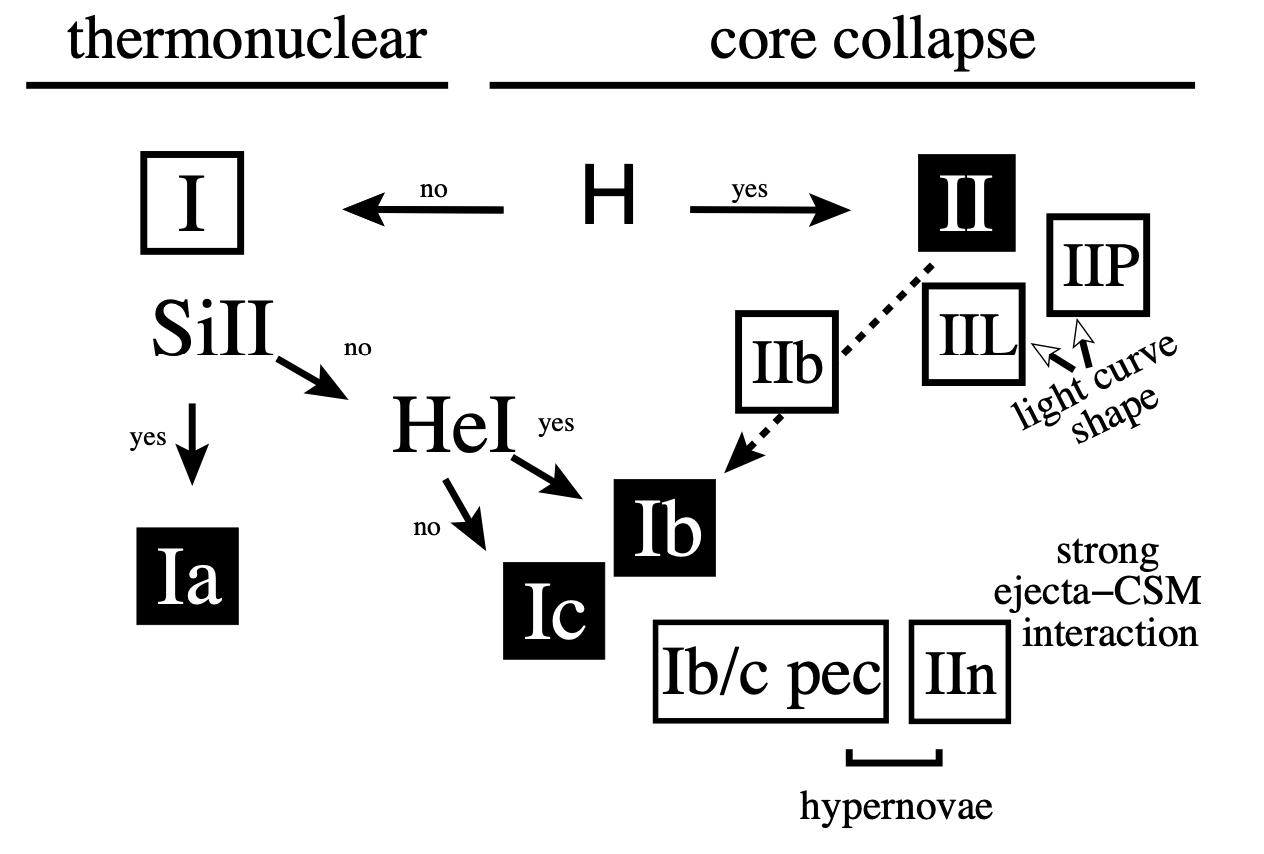
\includegraphics[width=0.8\linewidth]{figures/supernova_class.png }
    \caption[Supernova Classification]{Supernova classification. The 
    classification scheme is based on the presence or absence of hydrogen and 
    silicon features in the spectra of SNe. Figure from \textcite{Turatto2003}.}
    \label{fig:sn-classification}
\end{figure}

% The classification scheme in Figure~\ref{fig:sn-classification} is based on
% the presence or absence of hydrogen and silicon emission and absorption lines in the spectra of SNe.
SNe with hydrogen in their spectra are classified as Type II SNe, while those
without hydrogen are classified as Type I SNe. Type I SNe are further
subdivided into Type Ia, Ib, and Ic~\parencite{Turatto2003}. Although divided into three 
subtypes, Type I SNe are caused by two different mechanisms. Type Ia SNe are 
caused by the thermonuclear explosion of a white dwarf star, while Type Ib and Ic 
SNe are caused by the core-collapse of a massive star~\parencite{Filippenko1997}.
Type Ib and Ic SNe, because of this, are actually more related to Type II SNe,
and are collectively referred to as core-collapse SNe. We now know the physical
origin of the spectral differences between the subtypes: stars stripped of their 
hydrogen envelopes are appear as Type Ib SNe, while those stripped of both their 
hydrogen and helium envelopes are classified as Type Ic SNe.

% \section{Supernova Identification}
% \label{sec:supernova-identification}
Merely detecting a supernova is not enough, as astronomers must identify its
type to determine the progenitor. Traditionally, a supernova is observed by several 
means, with discovery in photometric observations and classification using follow-up 
spectroscopy (e.g. \textcite{Perlmutter1999}). This process is time-consuming, requiring not only 
the initial discovery of the supernova, but also follow-up observations to determine
the type before it fades away. Due to the large volume of new discoveries and 
the small number of single and multi-object spectrographs suitable for follow-up, only 
about 10\% of discovered SNe receive spectroscopic classification \parencite{TNS}. 
% Citation on this could be the Transient Name Server.

\section{Dark Energy Spectroscopic Instrument}
\label{sec:DESI}
% \section{Dark Energy Spectroscopic Instrument}
% \label{sec: DESI}

The Dark Energy Spectroscopic Instrument (DESI) is a spectroscopic system located in Kitt Peak 
in Arizona. Installed at the Mayall 4-m telescope, DESI is fitted with 5000 fiber roots and 10 3-arm 
spectrographs capable of resolving the [O II] $\lambda \lambda3726,3729$ doublet used for redshift
fits of galaxies \parencite{Guy2023}. This instrument is currently being used in the DESI Bright 
Galaxy Survey (BGS) to produce a map of a dark-energy dominated universe with median redshifts of $z \approx 0.2$ 
\parencite{hahn2022, desicollaboration2016}. 

Over the five year span of observations, DESI will inevitably observe SNe overlapping targets, leading to 
contaminated spectra. BGS is hypothesized to contain on order of $10^5$ supernova 
\parencite{desicollaboration2016}. An example of a supernova observed and publicly classified is shown in 
Figure~\ref{fig:desi_supernova}. Transients of any kind run the risk of influencing the redshift fit provided by DESI, 
making transient detection and identification of upmost importance to the quality of the pipeline.
The difficulties in ensuring follow-up observations of possible SNe candidates prompts the development of 
autonomous techniques geared towards the discovery and classification of these targets serendipitously. 

\begin{figure}
    \centering
    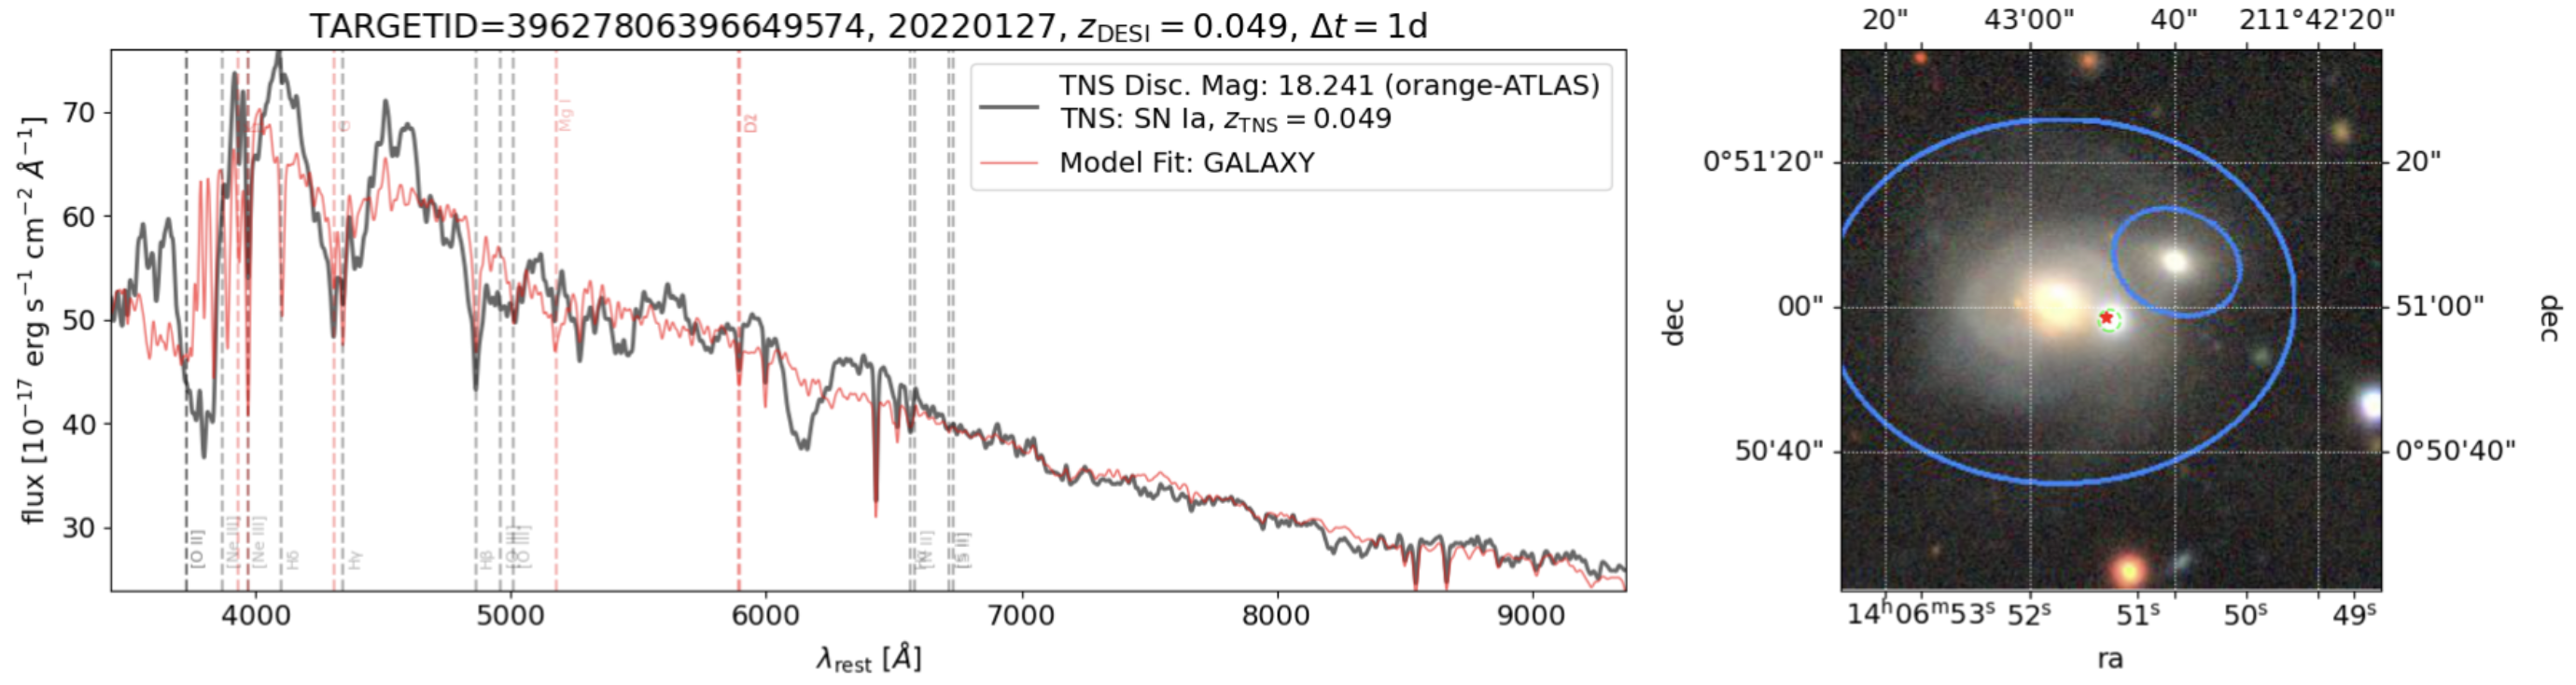
\includegraphics[width=\textwidth]{figures/desi_figures/SNe_Detection.png}
    \caption[Publicly Classified SNe captured by DESI]{DESI spectra and TNS public 
    classification of a type Ia supernova }
    \label{fig:desi_supernova}
\end{figure}

\section{Previous Approaches to Autonomous Supernova Identification}
\label{sec:PrevApproach}
The most straightforward example of an autonomous supernova identification algorithm would 
be the creation of templates for different SNe, and comparing observations against them. Raw spectra would have 
their foreground galaxies fitted and subtracted, and the residual spectrum can be identified as either background, 
or a transient.

However, this method leads to several computationally expensive issues. Firstly, the continuum 
must be accurately fitted in the presence of a possibly dominating transient. An incorrect fit 
regardless of the presence of a SNe can lead to a misclassification. Secondly, even if 
it is assumed that the residual spectrum contains only a supernova, there still needs to be 
a number of templates to be compared against. These templates must include all of the subtypes of 
SNe adjusted for all possible redshifts appropriate for the targets. In addition, the classification of 
SNe is also time dependent, so the evolution of each subtype must also be included in each template (an 
example shown in Figure~\ref{fig:sne_template}).

\begin{figure}[t]
    \centering
    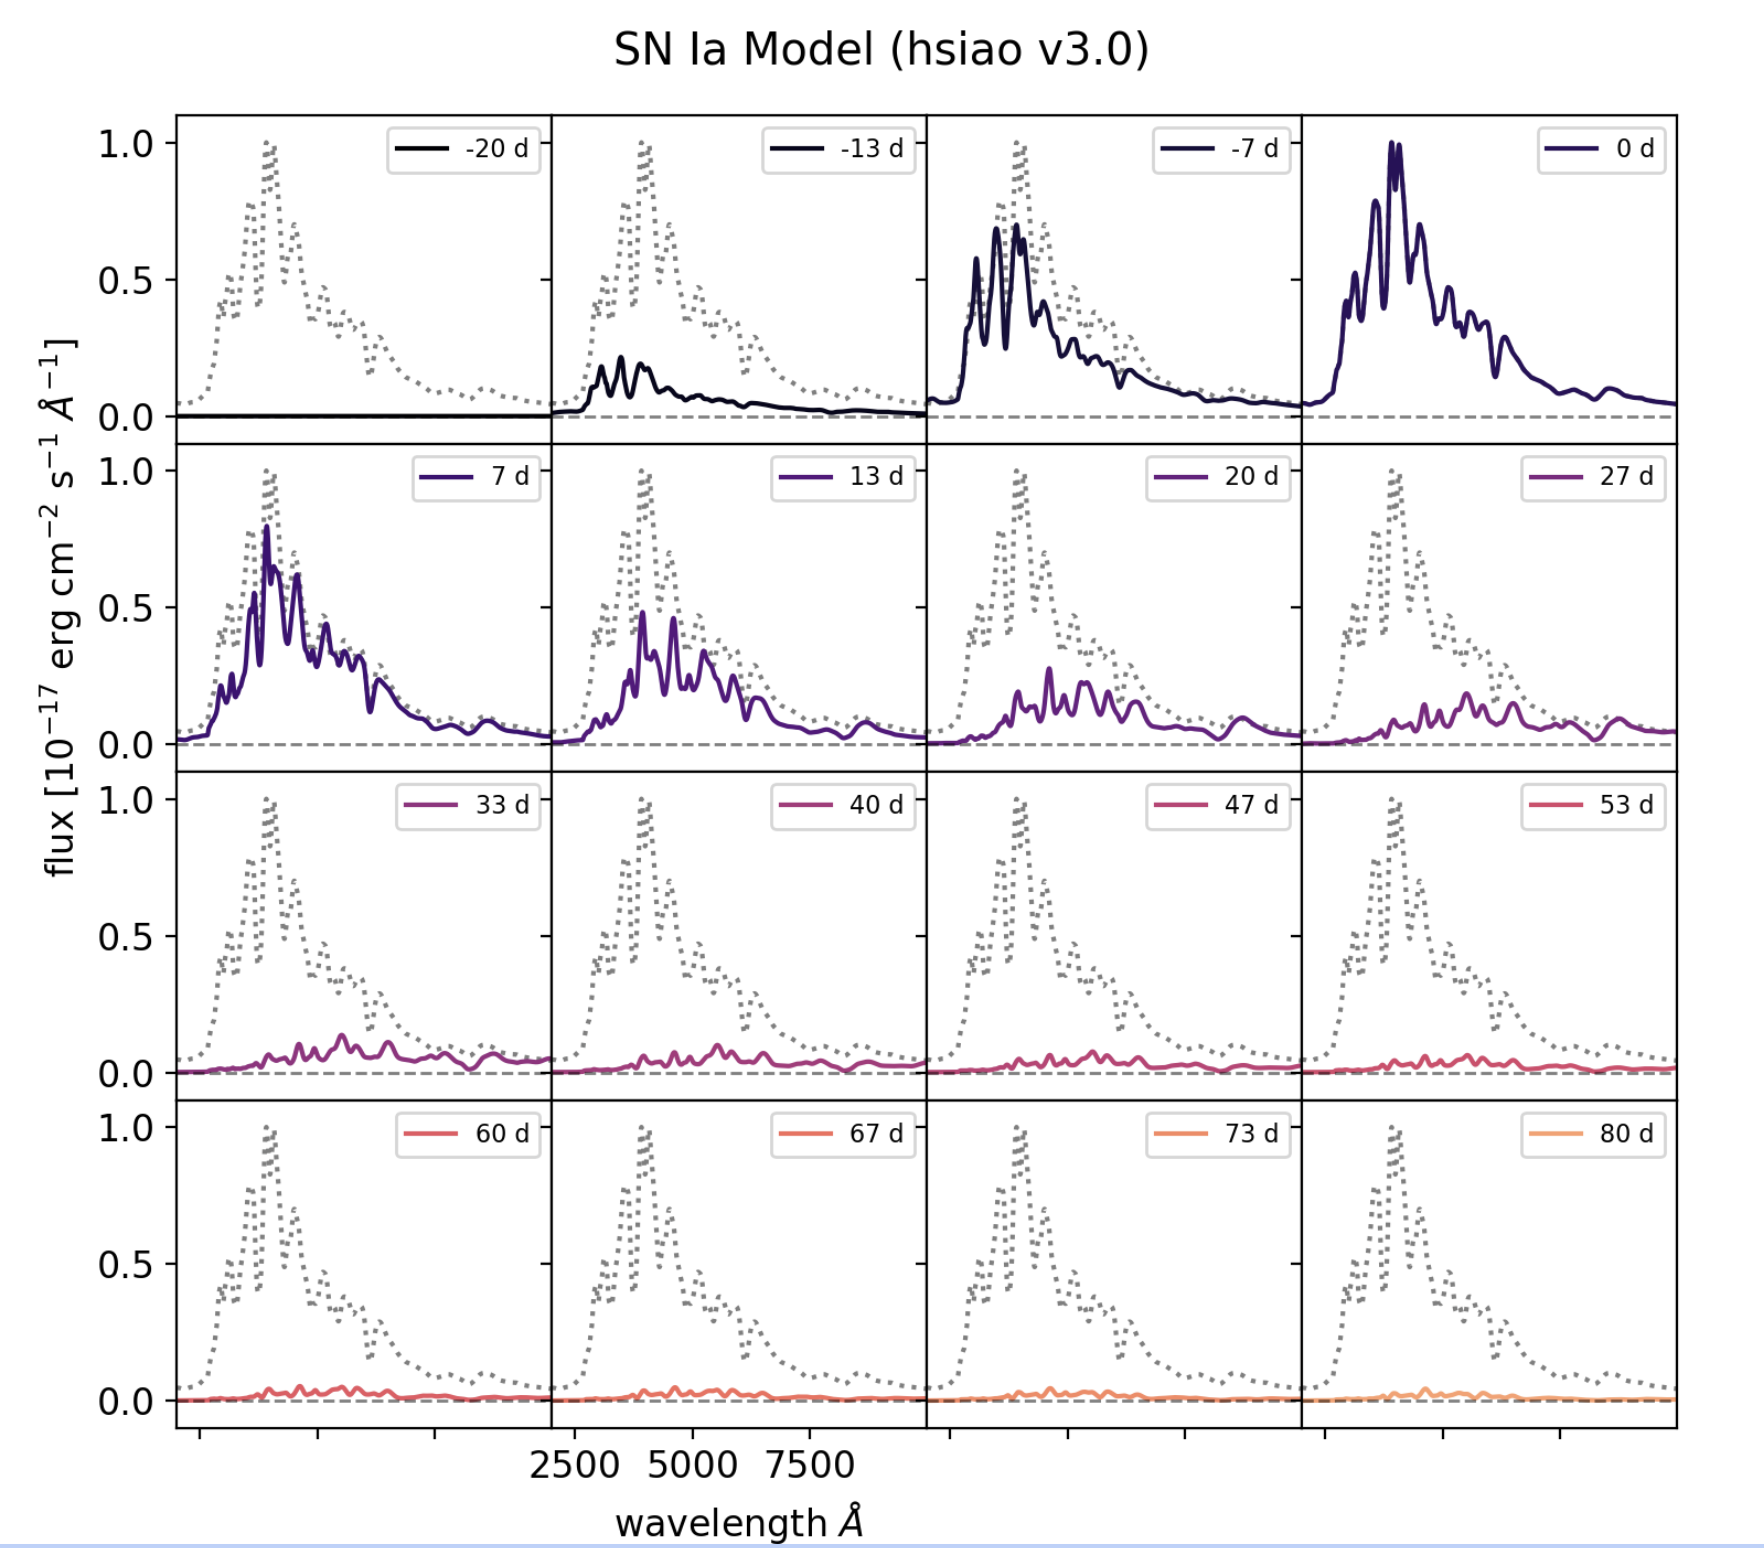
\includegraphics[width=.6\textwidth]{figures/desi_figures/snia_templates.png}
    \caption[Autonomous SNe Classification Templates]{Standard Approach to autonomous classification of 
    a type Ia supernova. Time evolution of the is shown over the course of 20 days before to 80 days after
    peak brightness. Adapted from \textcite{DESIpresentation}.}
    \label{fig:sne_template}
\end{figure}

% https://docs.google.com/presentation/d/14i0USbCQ93Mkn1T9aUK5pG24bi5bRfBhM3aVsL1Ya0U/edit?usp=sharing
% -- Look at spectra examples
% -- Look at motivation for no-redshift corrected transient classification

% https://docs.google.com/presentation/d/1zqoEVMrWbBP5k41gdjUEKioLE4J0vhu0vAzKEg4pROM/edit?usp=sharing
% -- An old presentation from 2020 that lists some past approaches to spectroscopic classification.
% -- Supernova tempates and compared them 
%   - Fit forgrown spectra from galaxy, fit residual spectrum. CHi^2 fit looks good?you discover it
% -- type IA evolution
%   - You can't just compare to one, you need to compare to A BUNCH because of time 
%   - So you want to compare to every template?? Convolve at different redshifts??
%   - SUUUPER expensive. ML/AI is just... better. 


\begin{comment}
% SB Comments:
% You want to motivate this in a couple of ways.
% 1) Because spectroscopic follow-up is tough, it's worthwhile to try to discover SNe serendipitously in spectra rather than only wait for discoveries in imaging surveys.
% 2) The issue with spectroscopic discovery is that you have potentially thousands of templates to compare against (all the different subtypes * all the variants of the subtypes * the spectral evolution of each variant * convolution vs redshift). Very computationally expensive!

% I suggest you give some background on previous approaches before jumping right into AI/ML.
% See the early slides in \href{https://docs.google.com/presentation/d/1zqoEVMrWbBP5k41gdjUEKioLE4J0vhu0vAzKEg4pROM/edit?usp=sharing}{this Google slideshow}.
\end{comment}

\section{Supernova Classification with Machine Learning}
\label{sec:supernova-classification-with-machine-learning}
Machine learning (ML) has been applied to many different fields for its flexibility 
and ability to find patterns in data. The emergence of Deep Learning (DL) has
allowed ML to be applied to more and more mundane tasks, such as image
classification~\parencite{krizhevsky2012}, speech recognition~\parencite{Nassif2019},
and natural language processing~\parencite{Mikolov2013}. ML and DL 
has also been applied to astronomy, with some success. \textcite{Gauci2010} used 
a random forest algorithm  to distinguish between spiral, elliptical, and irregular galaxies, 
and \textcite{Becker2021} used a convolutional neural network (CNN) to classify the morphology of
radio galaxies. CNNs found success in working within the DESI collaboration, with 
\textcite{parks2018} using the architecture to detect strong emission lines.  
These techniques have also been applied to the classification of SNe. 
\textcite{Mller2016} used a CNN to classify SNe into Type Ia and non-Type Ia SNe. 

Previous attempts at using machine learning algorithms for transient detection on DESI 
spectra have been conducted by \textcite{wasserman2021, Sepeku2022}. Both models were 
shown to be capable of high performance (further explained in Section~\ref{sec:CNNspectra}, 
but only after pipeline-dependent preprocessing and extensive cutting based on model certainty.
An alternative model based on the vision transformer (ViT) architecture is proposed to 
solve these short comings. Aptly named the ``Spectral ViT'', this model seeks to 
classify SNe into their respective subtypes with comparable precision and higher 
recall to previous models, without dependence on the DESI redshift fit for pre-processing. 

In Chapter~\ref{chap:DLTechniques}, the deep learning techniques used throughout the study 
are explained in detail, while Chapter~\ref{chap:methods} describes the creation and training 
of the ``Spectral ViT.'' The results of the study are discussed in Chapter~\ref{chap:results}, with 
future research and applications of this model presented in Chapter~\ref{chap:conclusions}. 


\begin{comment}
\section{Problem Statement}
This work will explore the following questions: how can we adapt novel deep learning 
techniques to classify SNe in the DESI dataset? Can we use this architecture to 
classify SNe into their respective subtypes accurately? And how can we decrease the amount of 
pre-processing required to classify these SNe accurately? In the following chapters,
we describe the Deep Learning techniques adopted to answer this problem (Ch. 2);
the training procedure for building our classification network (Ch. 3);
and the results using simulated DESI spectra that were resampled from actual 
DESI measurements performed in 2021 and 2022 (Ch. 4).
\end{comment}




\chapter{Deep Learning Techniques}
\label{chap:MLTechniques}
%%%%%%%%%%%%%%%%%%%%%%%%%%%%%%%%%%%%%%%%%%%%%%%%%%%%%%%%%%%%%%%
% Outline 
% Introduce Machine Learning, and why traiditonal MLP is not good enough
% 1. Convolutional Neural Networks
% 1.1 Example architecture and sucess in vision tasks
% 1.2 1D CNN implemented on DESI spectra
% 1.3 2D CNN implemented on DESI spectra (Eddies Research)
% 2. Transformers 
% 2.1 Example architecture and sucess in NLP tasks + Vision Tasks --> Connection 
%      to DESI
% 2.2 Multi-Head Attention and Self-Attention for spectral classification
% 2.3 Possilbility of NOT having to k-correct for redshift because of this attention
% 2.4 Adjected ViT architecture for DESI

%%%%%%%%%%%%%%%%%%%%%%%%%%%%%%%%%%%%%%%%%%%%%%%%%%%%%%%%%%%%%%%
\section{Multi-Layer Perceptrons}\label{sec:MLP}
To aid in the classification of supernovae, deep learning techniques can provide 
flexibility and scalability that have been previously unattainable by manual 
methods. The simplest and most widely used architecture in deep learning are feed-forward 
fully connected neural networks, also known as multi-layer perceptrons (MLPs) \parencite{popescu2009}.
These networks are composed of series of ``layers'' of neurons, or nodes, that 
are ``fully connected'' to the previous layer (Figure \ref{fig:MLP}).
Given an input vector $\vec{x}^{(0)}$ with $n$ values, an MLP applies a series of weights to each 
element, resulting in a linear transformation from $\vec{x}^{(0)}$ to $\vec{x}^{(1)}$, where
$\vec{x}_{(1)}$ is a vector of length $m$. This transformation is then followed by a bias added 
to each element, and an activation function applied to each element.
The transition from layer $i$ to $i+1$ can be represented mathematically as 
\begin{equation}\label{eqn:MLP}
    \vec{x}^{(i+1)} = f(\mathbf{W}\vec{x}^{(i)} + \vec{b}^{(i+1)}),
\end{equation}
where $\mathbf{W}$ is an $m \times n$ matrix of weights, $\vec{b}^{(i+1)}$ is a vector of length $m$
representing the bias, and $f$ is the activation function. The activation function can 
be any function, but traditionally they are chosen to be continuous, non-linear, 
monotonically increasing, and differentiable. The most common activation functions 
are the sigmoid function, $f(x_i) = \sigma(x_i) = 1/(1 + e^{-x_i})$, hyperbolic tangent, 
$f(x_i) = \tanh(x_i)$, and the rectified linear unit,
$f(x_i) = \mathrm{ReLU}(x_i) \equiv \max(0,x_i)$, all of which are applied element-wise.
\begin{figure}[t]
    \centering
    \input{tikz/MLP.tex}
    \caption{A simple MLP with an input dimension of 4 (green nodes), three hidden layers (blue nodes), and an output dimension of 3 (red nodes). Each node is connected to every 
    node in the previous and next layer. The lines represent the weights, and each 
    node has an associated bias. Figure adapted from \textcite{neutelings2021_nn}.}
    \label{fig:MLP}
\end{figure}
The output layer of the network is a vector tailored for the particular purpose
of the MLP. For example, if the network is used to classify input data $\vec{x}$ into a set of classes, the output is a vector of normalized probabilities of each class. 

The MLP architecture, while simplistic, is very powerful. \textcite{cybenko1989} showed that for any boolean 
function (i.e. 2-class classification), an MLP with a single hidden layer could 
approximate any function arbitrarily well; this is known as the Universal Approximation
Theorem. The theorem is the basis for the success of MLPs in
many fields, but it is also the reason that MLPs are not the best choice for all problems.
MLPs begin to show many complications when training large models, such as the 
exploding/vanishing gradient problem that makes them difficult to train (CITE Nielsen?), a lack of invariance under translation (important for many types of data, such as images), 
and exponential growth of the number of trainable parameters \parencite{Naskath2022}. These problems inhibit the use of MLPs on larger datasets and in more complex problems, including 
image recognition, time series analysis, and natural language processing. Since 
the mid-2000s, the weaknesses of MLPs have been addressed by the adoption of 
alternative network architectures such as convolutional neural networks (CNNs) and
transformers.

\section{Convolutional Neural Networks}\label{sec:CNN}
Convolutional neural networks (CNNs) were originally developed
to address the lack of invariance under translation in input data \parencite{fukushima1979}.
CNNs designed for classification are traditionally composed of a series of convolutional layers, 
usually followed by a pooling layer, and a fully connected layer. The convolutional 
layers are composed of a series of filters that take a certain 
number of inputs from the previous layer and apply a kernel to them, resulting in 
a single output. These filters are applied across the entire input space, and are 
commonly referred to as feature maps. 
%Inputs are traditionally padded to preserve 
%the dimensionality of the original tensor size.
If $N$ filters are applied in 
each convolutional layer, the result is a tensor of shape $N\times x$, where 
$x$ is the shape of the original input (which can be 1D or multi-dimensional). 
To reduce the dimensionality of the output, a pooling layer is applied.
The pooling layer takes a certain number of inputs from the previous layer, and 
reduces them to a single output, similar to the convolutional filters, but 
without the kernel application. The most common pooling layer is the max-pooling
layer, which takes the maximum value in each set as the reduced value. 
The process of passing an input through a convolutional filter and pooling layer is shown in Figure~\ref{fig:convolution}. 
These convolution and pooling layers are applied in series until the desired output dimensionality is reached.
\begin{figure}[t]
    \centering 
    \begin{tikzpicture}[
    2d-arr/.style={matrix of nodes, row sep=-\pgflinewidth, column sep=-\pgflinewidth, nodes={draw}}
  ]

  \matrix (mtr) [2d-arr] {
  |[fill=red!30]| 0  & |[fill=red!30]| 0  & |[fill=red!30]| 0  & |[fill=red!30]| 0  & |[fill=red!30]| 0  & |[fill=red!30]| 0 \\
  |[fill=red!30]| 0  & |[fill=orange!30]| 1 & |[fill=orange!30]| 1 & |[fill=orange!30]| 1 &  0 & |[fill=red!30]| 0 \\
  |[fill=red!30]| 0  & |[fill=orange!30]| 0 & |[fill=orange!30]| 1 & |[fill=orange!30]| 1 &  1 & |[fill=red!30]| 0 \\
  |[fill=red!30]| 0  & |[fill=orange!30]| 0 & |[fill=orange!30]| 1 & |[fill=orange!30]| 1 & 0 & |[fill=red!30]| 0 \\
  |[fill=red!30]| 0  & 1 & 1 & 0 & 0 & |[fill=red!30]| 0 \\
  |[fill=red!30]| 0  & |[fill=red!30]| 0  & |[fill=red!30]| 0  & |[fill=red!30]| 0  & |[fill=red!30]| 0  & |[fill=red!30]| 0 \\
  };

  \node[below=of mtr-5-4] {$4\times4$ input with padding};

  \node[right=0.2em of mtr] (str) {$*$};

  \matrix (K) [2d-arr, right=0.2em of str, nodes={draw, fill=teal!30}] {
    1 & 0 &1\\
    0 & 1 &0\\
    1 & 0 & 1\\
  };
  \node[below=of K-2-2] {$3\times3$ filter};

  \node[right=0.2em of K] (eq) {$=$};

  \matrix (ret) [2d-arr, right=0.2em of eq] {
  2 & 2 & 3 &  1\\
  2 & |[fill=blue!80!black!30]| 4 & 3 & 3\\
  2 & 3 & |[fill=orange!30]| 4 & |[fill=orange!30]| 1 \\
  2 & 2 & |[fill=orange!30]| 1 & |[fill=orange!30]| 1 \\
  };
  \node[below=of ret-4-3] {$4\times4$ tensor};

  \node[right=0.2em of ret] (ra) {$\xrightarrow[]{\text{Max Pooling}}$};

\matrix (pool) [2d-arr, right=0.2em of ra] {
  4 & 3 \\
  3 & |[fill=blue!80!black!30]| 4 \\
  };
  \node[below=of pool-2-2] {$2\times2$ tensor};

  \draw[dashed, teal] (mtr-2-4.north east) -- (K-1-1.north west);
  \draw[dashed, teal] (mtr-4-4.south east) -- (K-3-1.south west);

  \draw[dashed, blue!80!green] (K-1-3.north east) -- (ret-2-2.north west);
  \draw[dashed, blue!80!black] (K-3-3.south east) -- (ret-2-2.south west);

  \draw[dashed, blue!80!green] (K-1-3.north east) -- (ret-2-2.north west);
  \draw[dashed, blue!80!black] (K-3-3.south east) -- (ret-2-2.south west);

\draw[dashed, blue!80!green] (ret-3-4.north east) -- (pool-2-2.north west);
  \draw[dashed, blue!80!black] (ret-4-4.south east) -- (pool-2-2.south west);

\end{tikzpicture}

    \caption{A convolutional filter and a $2\times2$ pooling applied to a 2D input. As the filter is passed 
        over the input space, the kernel is applied. The input is padded with zeros to preserve dimensionality, 
        which is then reduced by the max pooling. Figure adapted from \textcite{neutelings2022_conv}.}
    \label{fig:convolution}
\end{figure}

From here, depending on the task, the output of the pooling layer can be fed
into a fully connected layer, similar to the MLP architecture described
in Section~\ref{sec:MLP}, or it can be fed into another convolutional layer. An
MLP is usually applied for classification tasks, while another convolutional layer
is applied for segmentation tasks. An example of a CNN architecture used for 
classification is shown in Figure~\ref{fig:CNN}.

\begin{figure}[t]
    \centering
    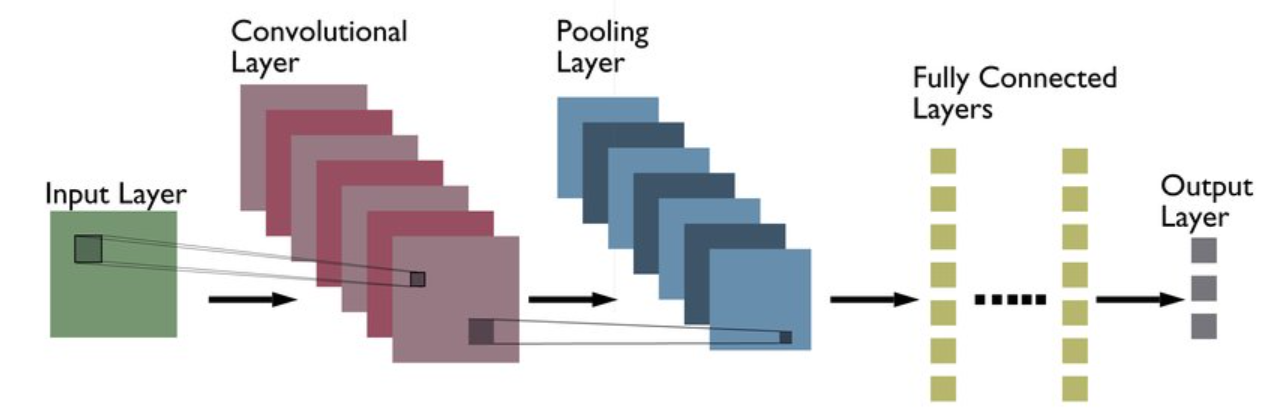
\includegraphics[width=.8\linewidth]{figures/Typical-CNN-architecture.png}
    \caption{A convolutional network archeticture designed for classification (adapted from \cite{kumar2022_cnn}). Only
    one convolutional/pooling layer is shown, but there can be multiple depending on the application. }
    \label{fig:CNN}
\end{figure}


The CNN architecture was shown to be effective in image recognition tasks by
\textcite{lecun2004} and then popularized after the success of AlexNet in the 
ImageNet challenge \textcite{krizhevsky2012}. AlexNet was the first of many CNN 
architectures popularized in the 2010s for vision classification, such as VGG \parencite{Simonyan15}, 
ResNet\parencite{he2016deep}, and DenseNet \parencite{Huang2016}. This also spurred a sudden increase in deep networks designed 
for segmentation tasks as well, such as the FCN architecture by \textcite{Shelhamer2016}. In addition to vision tasks, it also found 
great succes in applications such as natural language processing \parencite{Kim2014}, engineering, and 
medicine \parencite{Kiranyaz2021}. 

\subsection{CNNs on Spectroscopic Data in Astronomy}
\label{sec:CNNspectra}
CNNs excel at identifying patterns throughout their input space, stemming from their spacial invariance. 
Theoretically, this should translate to spectral classification quite well. In fact, CNNs have been applied 
to spectroscopic data in the past, including on the DESI dataset. 
\textcite{parks2018} used a CNN to detect strong emission lines in DESI spectra with 
great success. * Talk about 1D CNN currently running, and preprocessing used *

This work provides a baseline for the use of CNNs on supernovae classification, 
\textbf{but leaves more to be desired.} Therefore, an alternate architecture was proposed 
by * Cite Eddies work * which augments the preprocessing of the spectra with 
a conversion to a 2D image. This 2D image was then fed to a more traditional vision 
CNN architecture (Appendix~\ref{app:CNN}). 
% TODO: Make into Subcaptions
\begin{figure}[t]
    \centering
    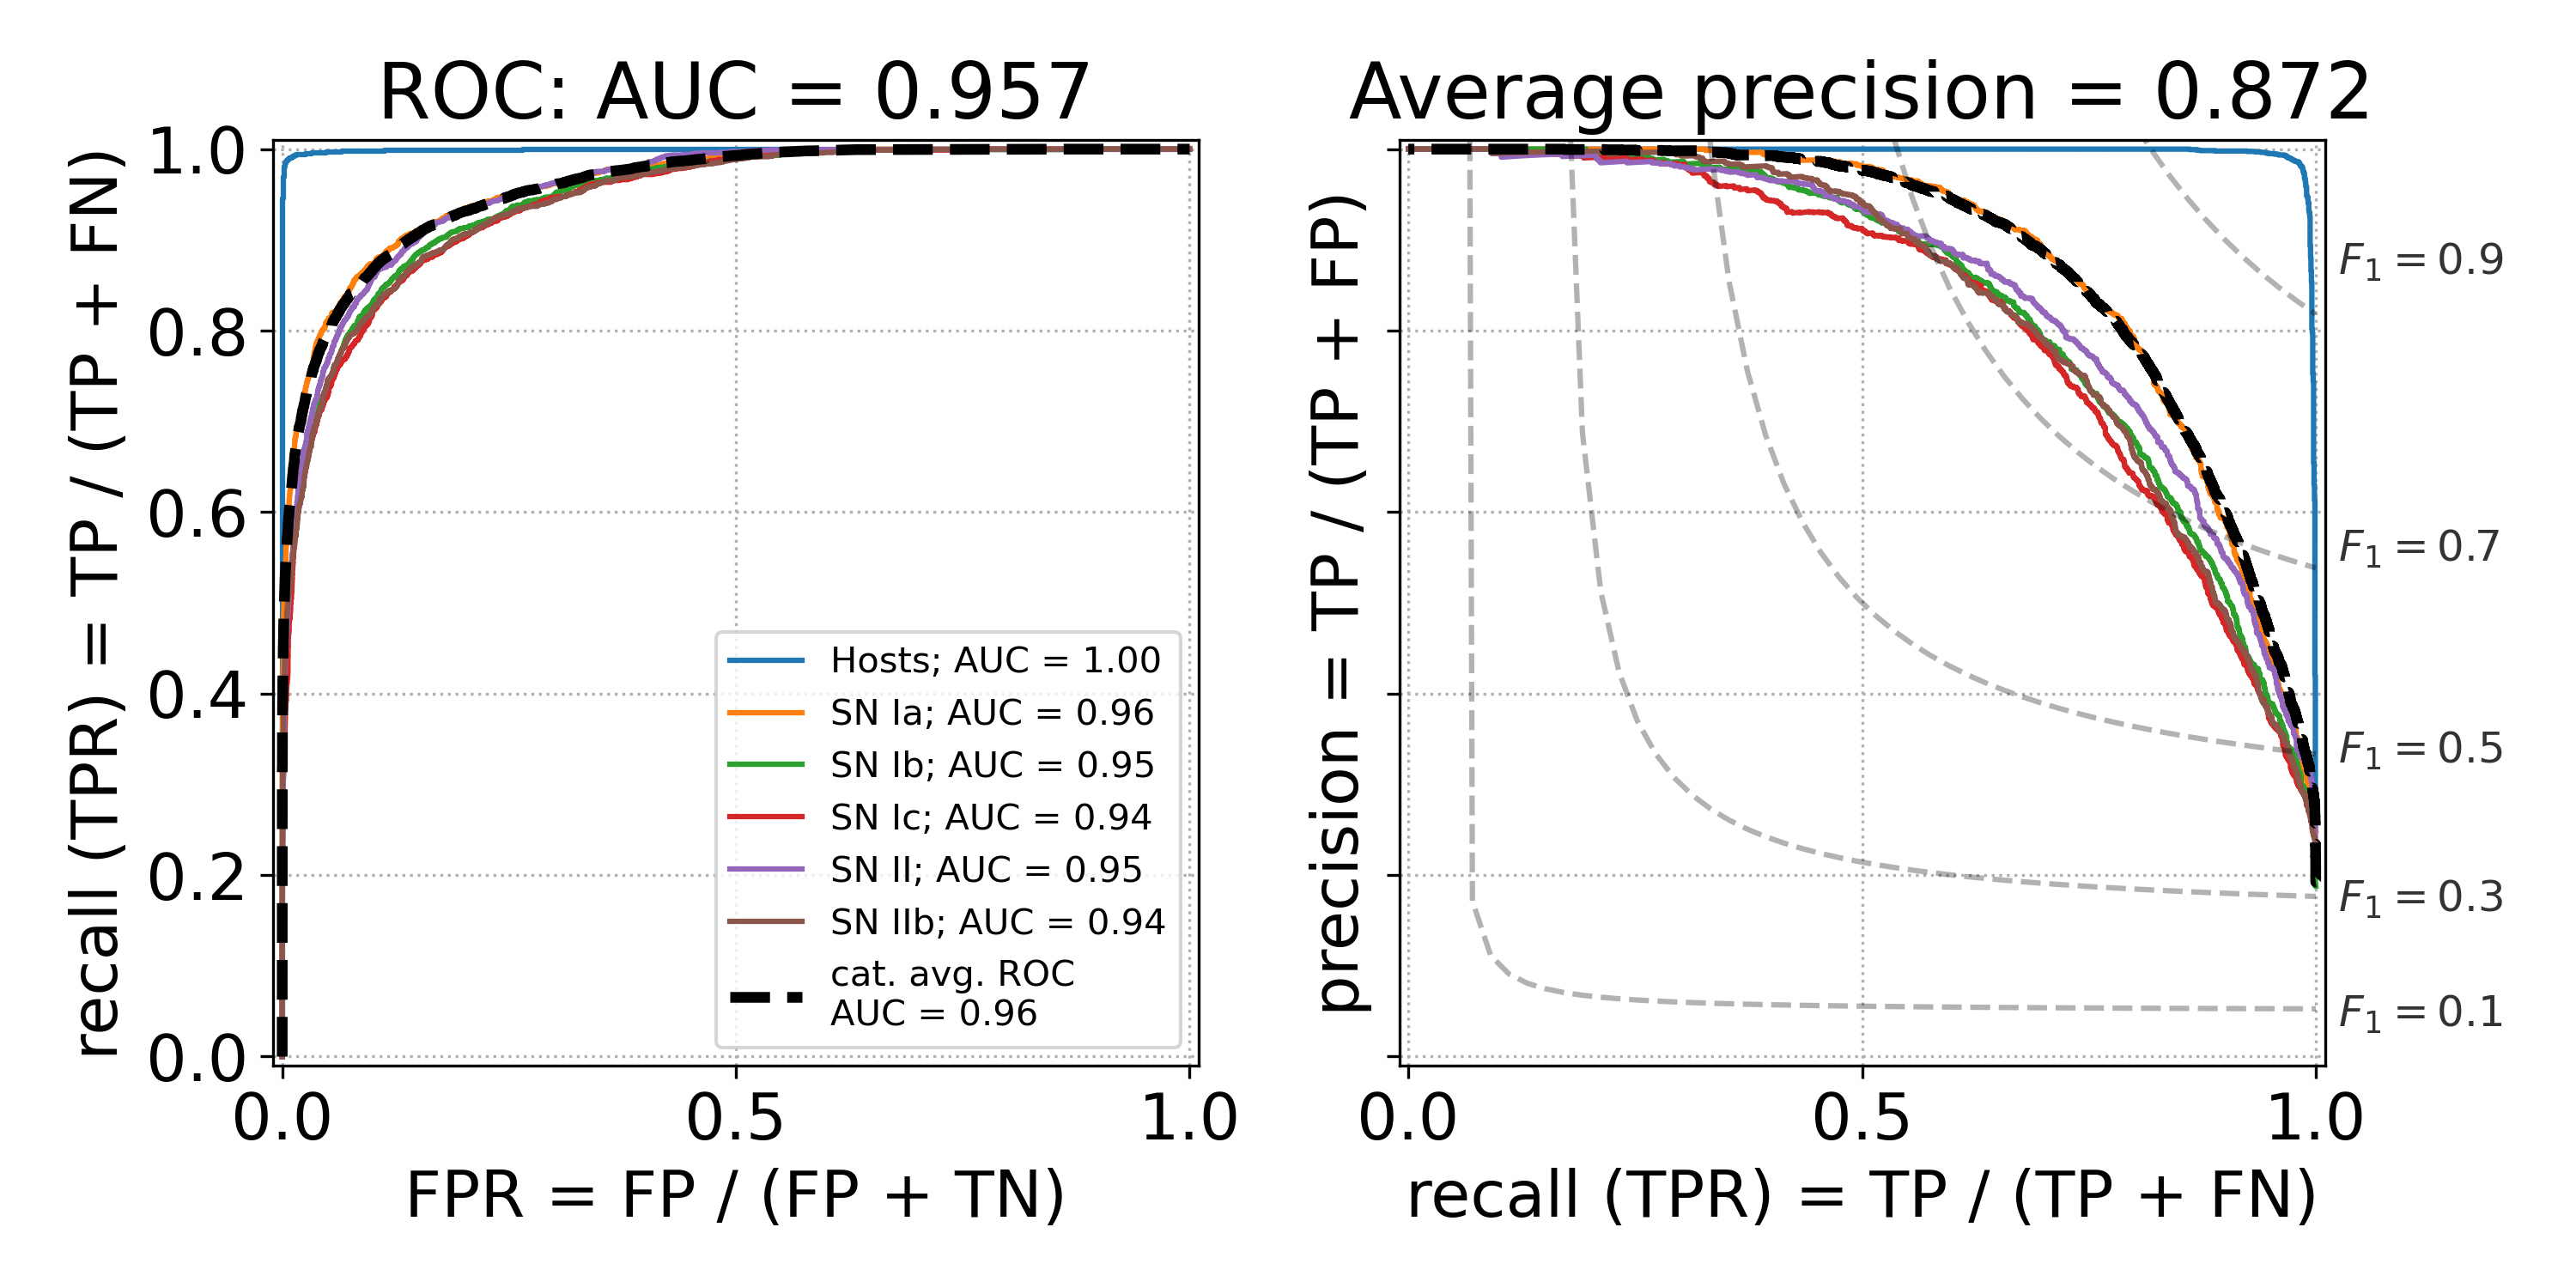
\includegraphics[height=4.55cm]{figures/cnn/cnn_rocfull.png}
    \quad
    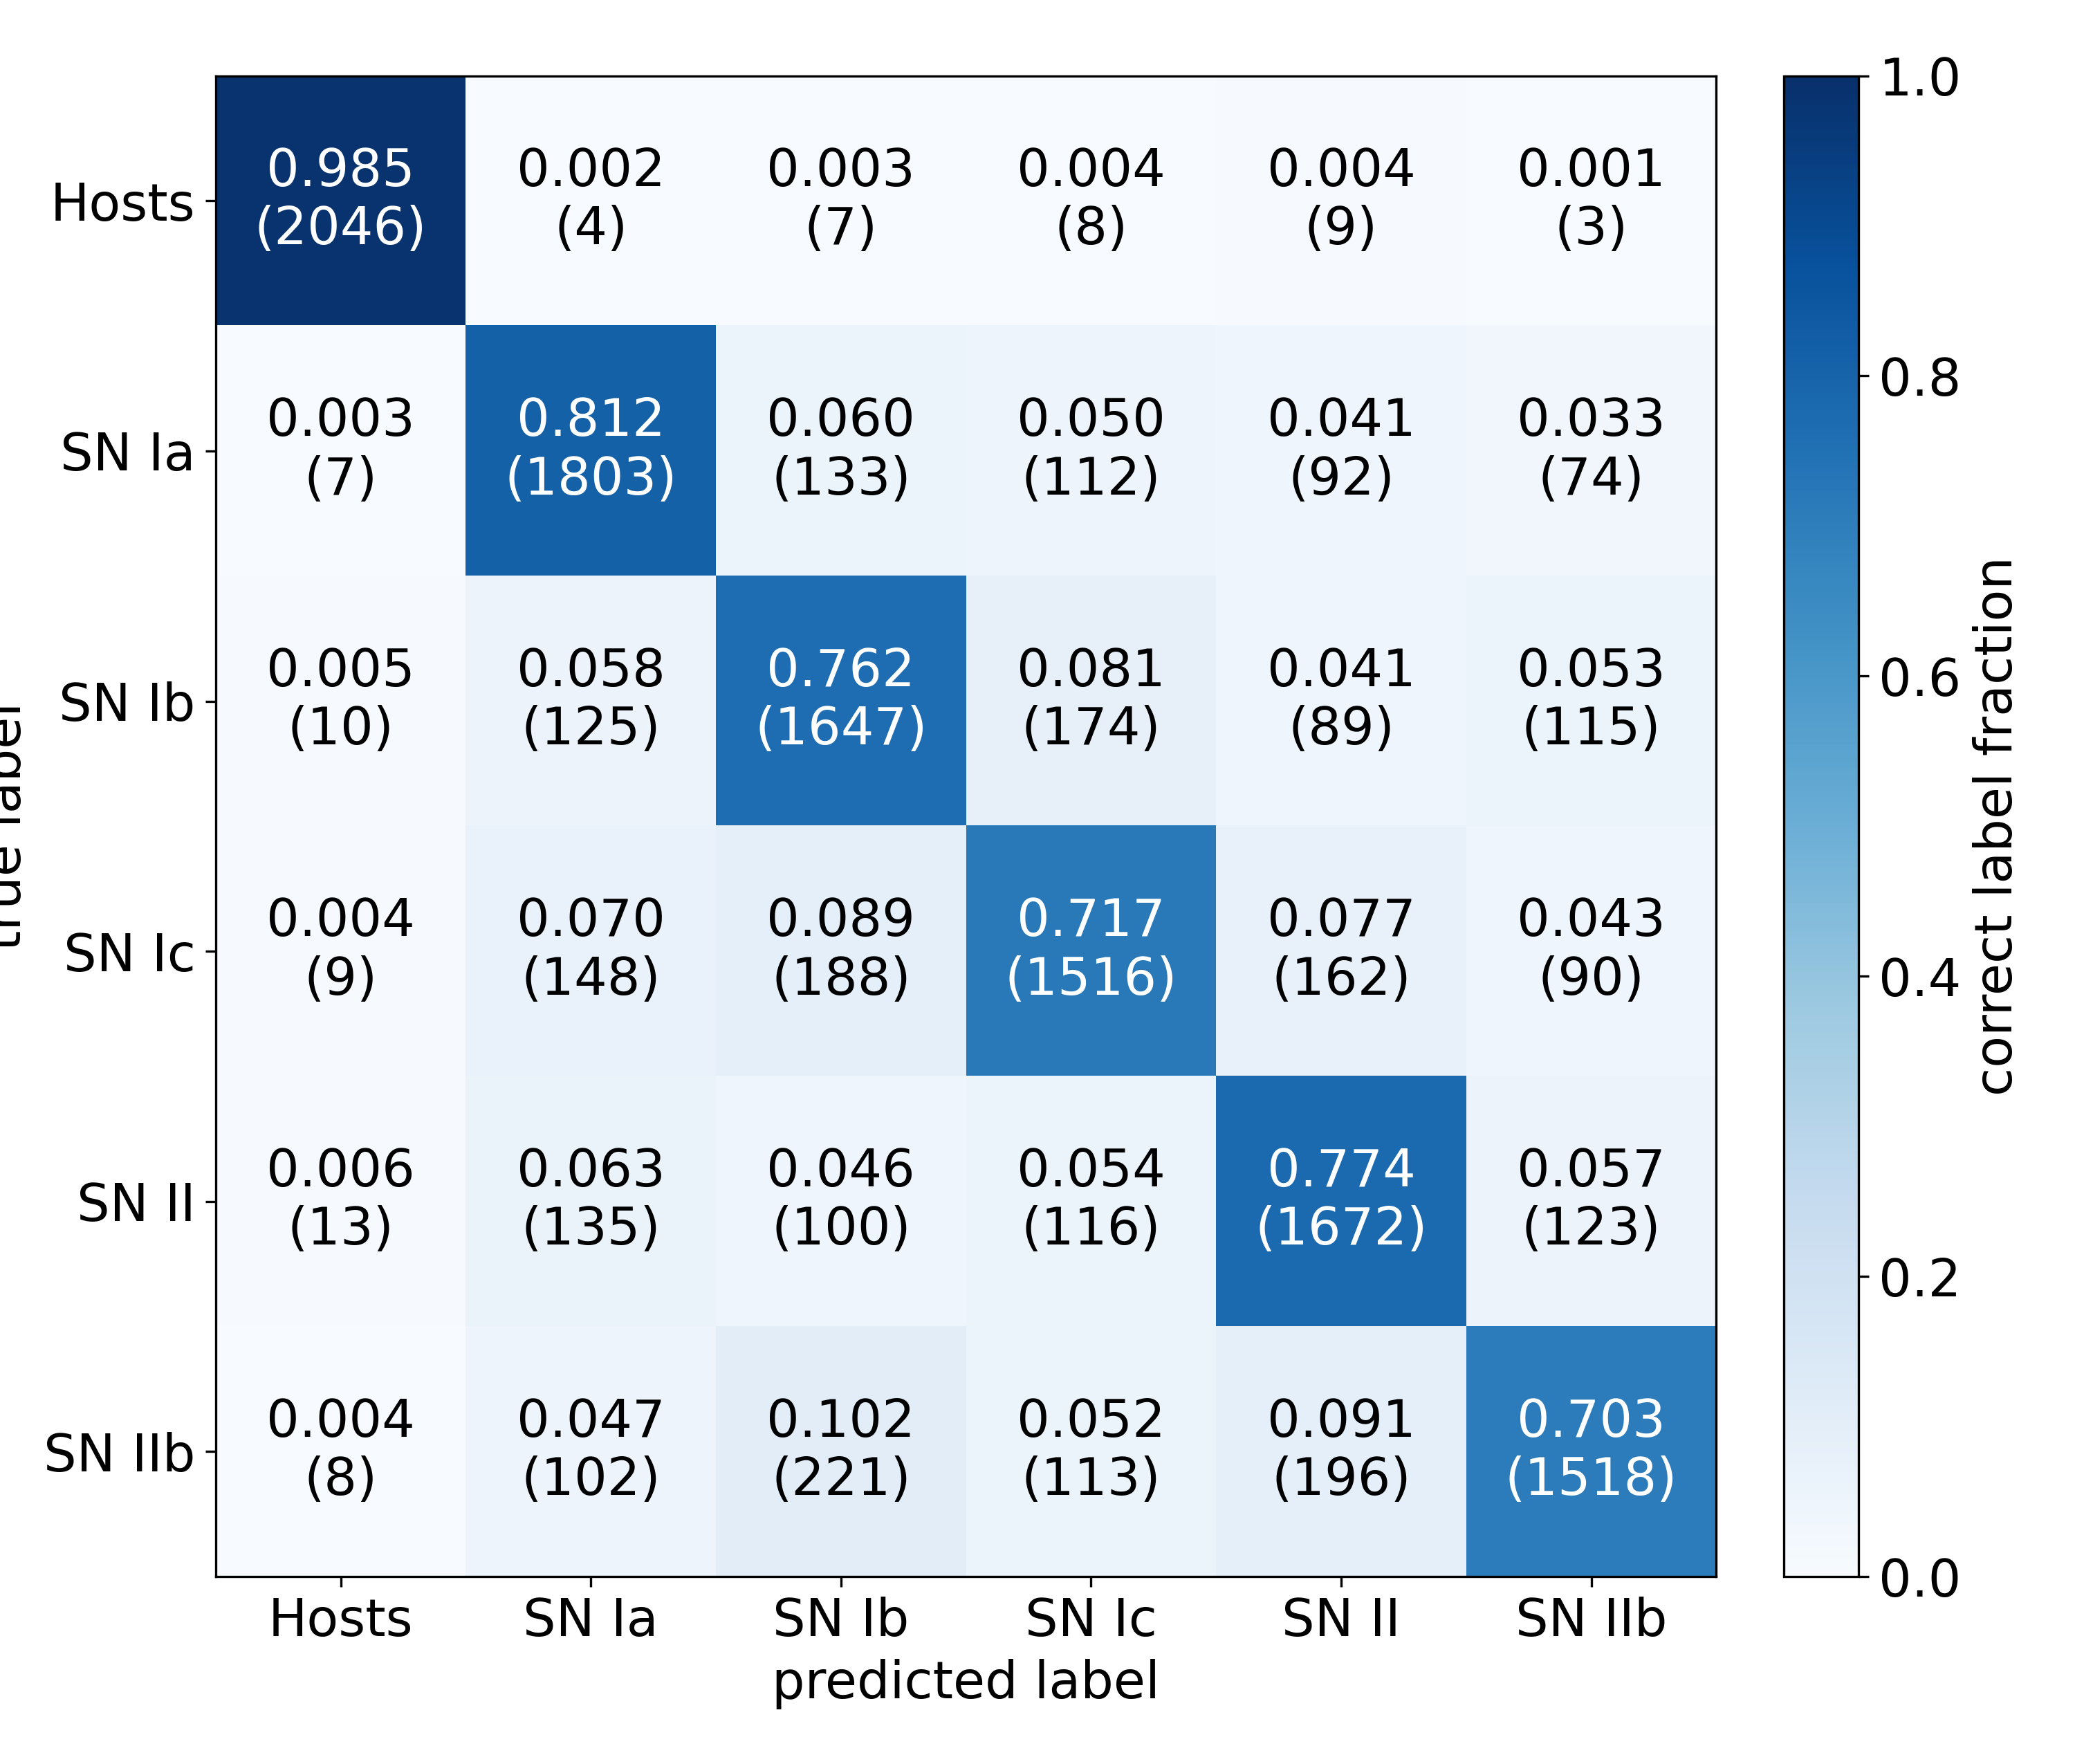
\includegraphics[height=4.55cm]{figures/cnn/cnn_cmfull.png}
    \caption{CNN Diagnostics: ROC Curve (left) and Confusion Matrix (right)\label{fig:cnn_qual}}
\end{figure}
This architecture was shown to train quickly (less than 1 hour on a single GPU), 
but it was not able to achieve astonishingly high accuracy. Figure~\ref{fig:cnn_qual}
shows the ROC curve and confusion matrix for the CNN trained on synthetic spectra. 
\begin{figure}[b]
    \centering
    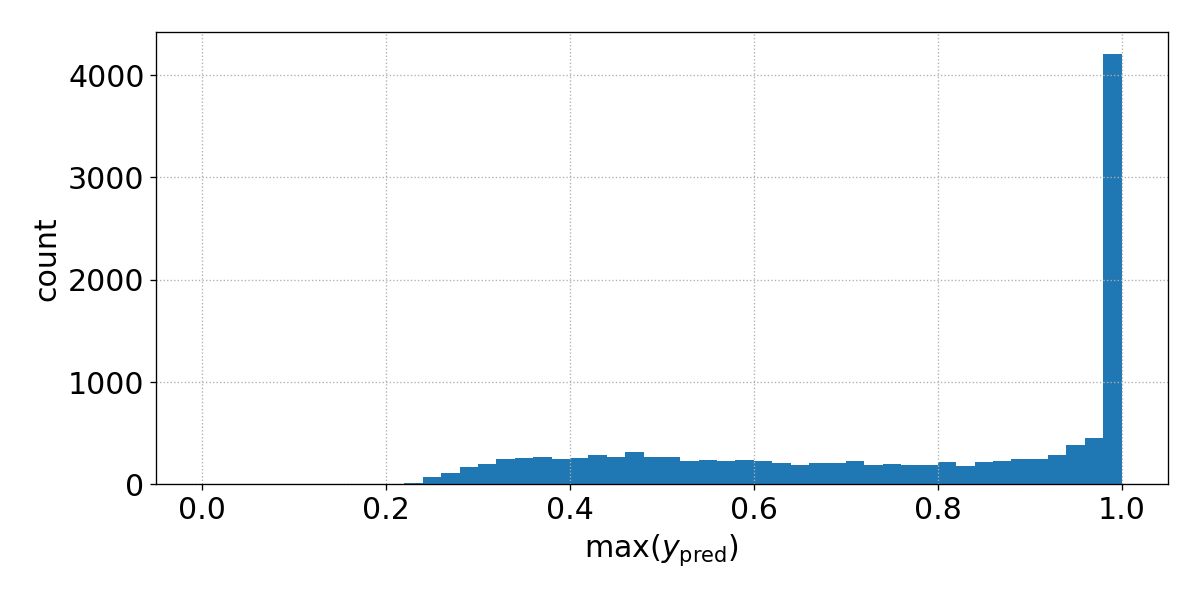
\includegraphics[width=0.6\textwidth]{figures/cnn/cnn_max_ypred.png}
    \caption{Max value of the output vector from the CNN.\label{fig:cnn_max}}
\end{figure}

The maximum value of the output vector was used to determine the predicted class,
\textbf{which may not be the best choice for this problem. why not?} Figure~\ref{fig:cnn_max} shows
the distribution of the maximum value found. As shown, there are approximately 
20 thousand spectra that are classified very confidently, but there are many
more that are not.
% TODO: Make into Subcaptions
\begin{figure}[t]
    \centering
    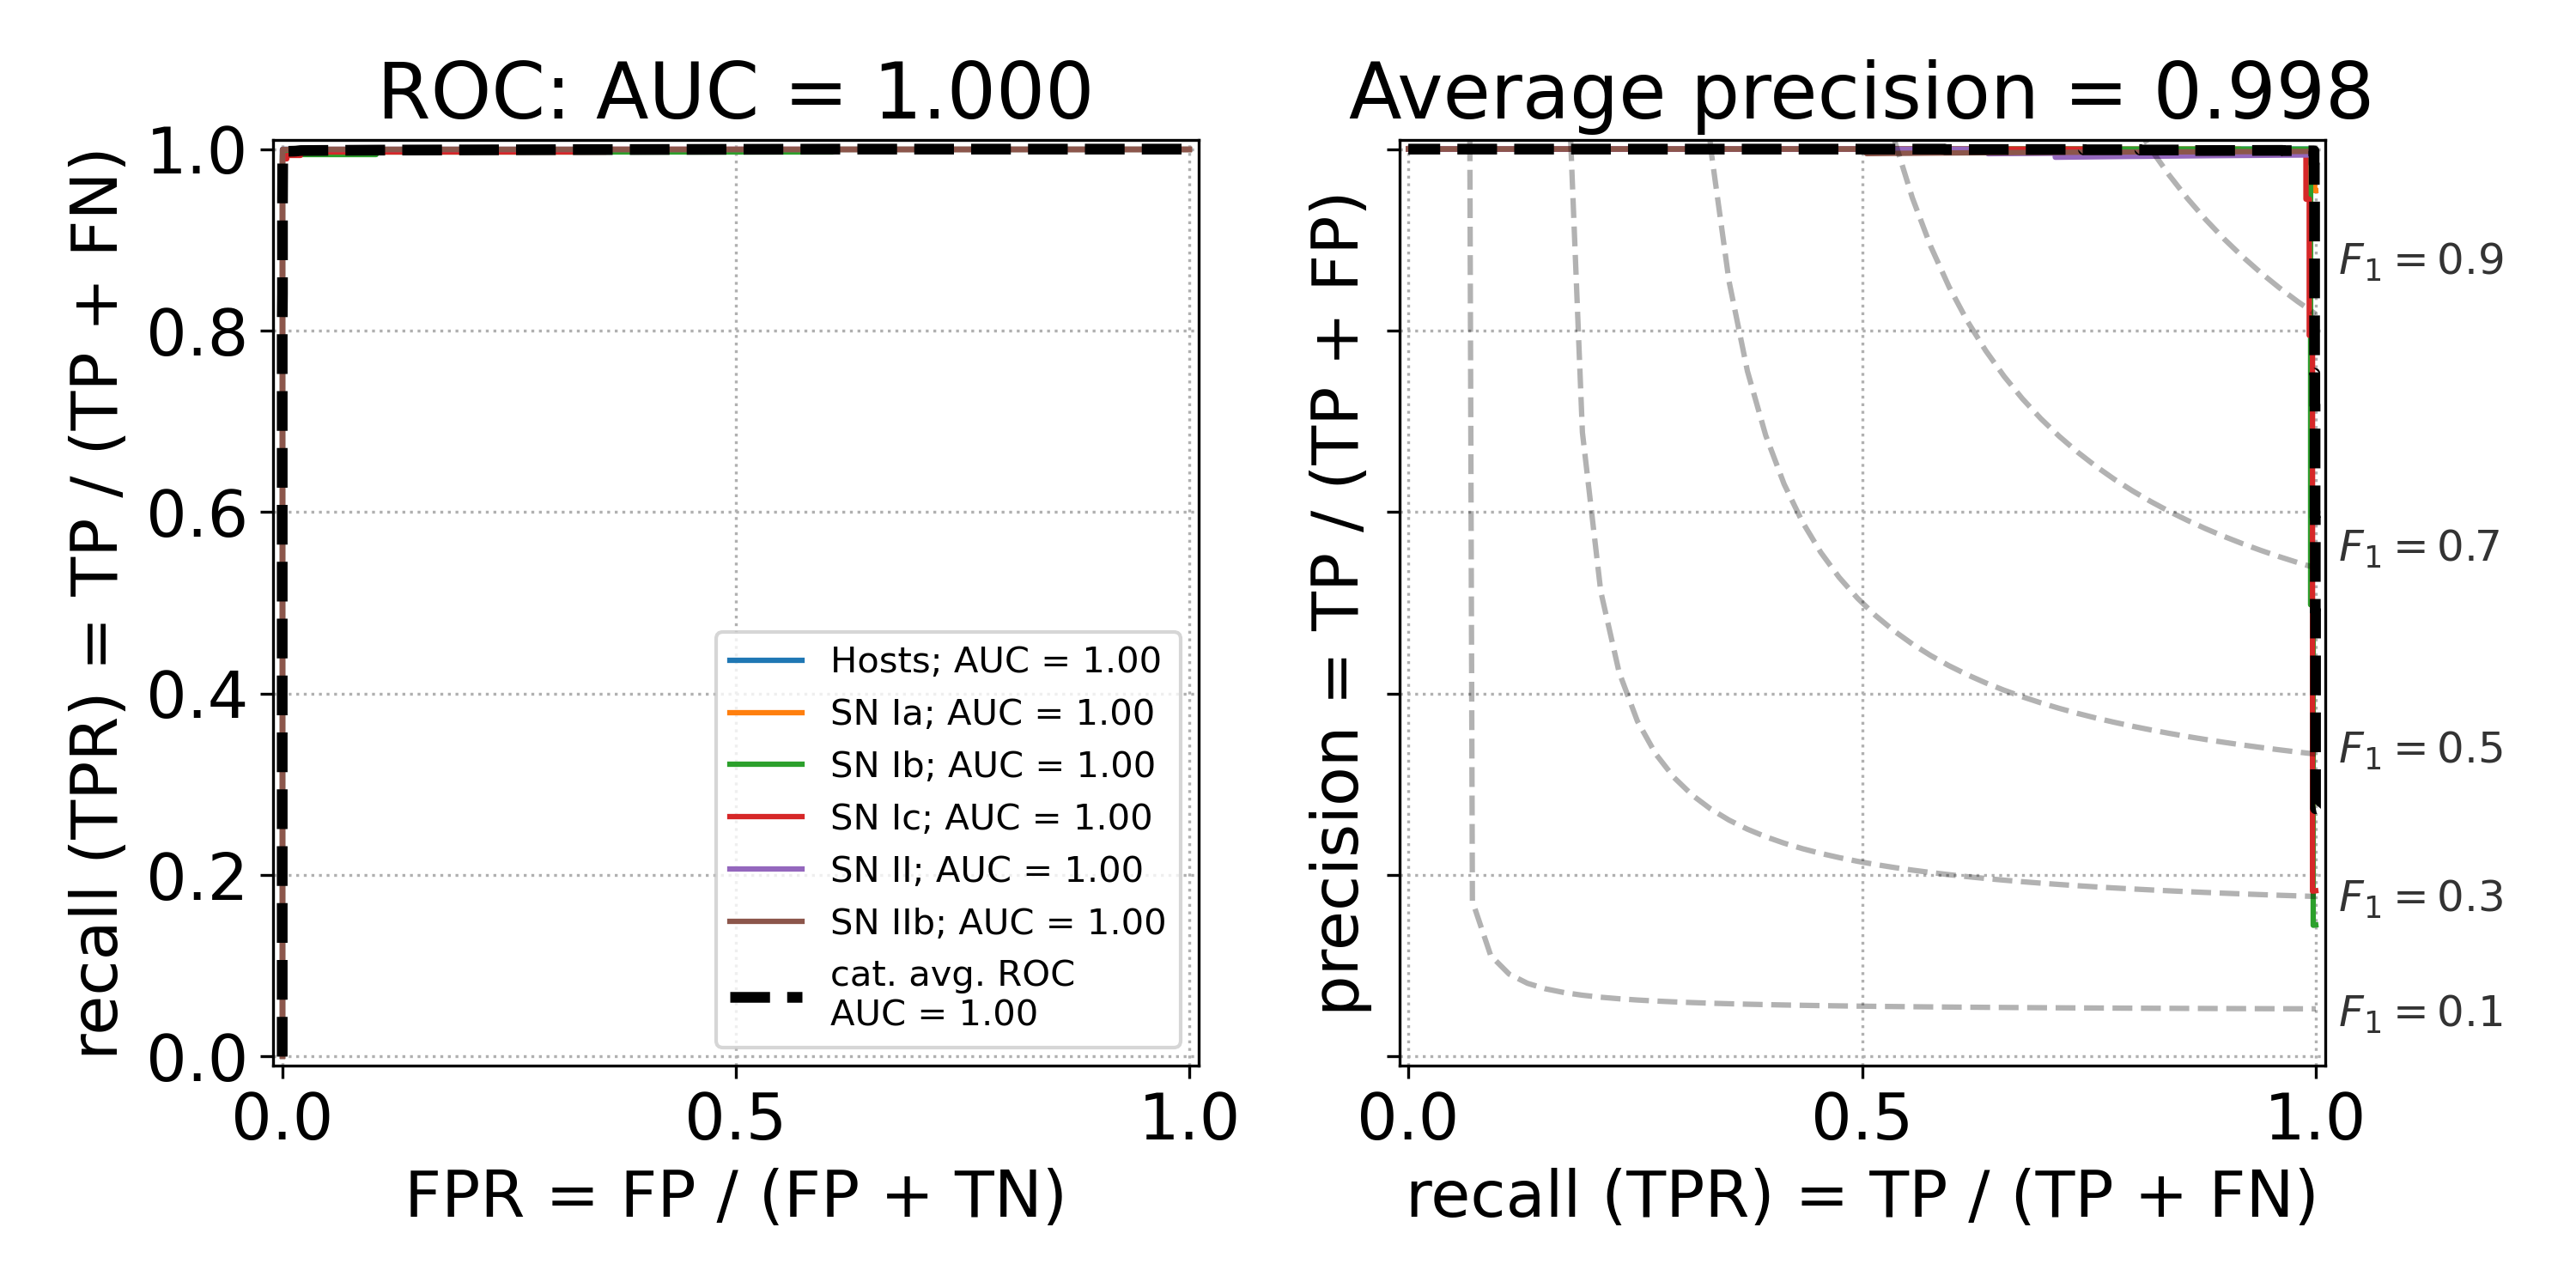
\includegraphics[height=4.55cm]{figures/cnn/cnn_roc99.png}
    \quad
    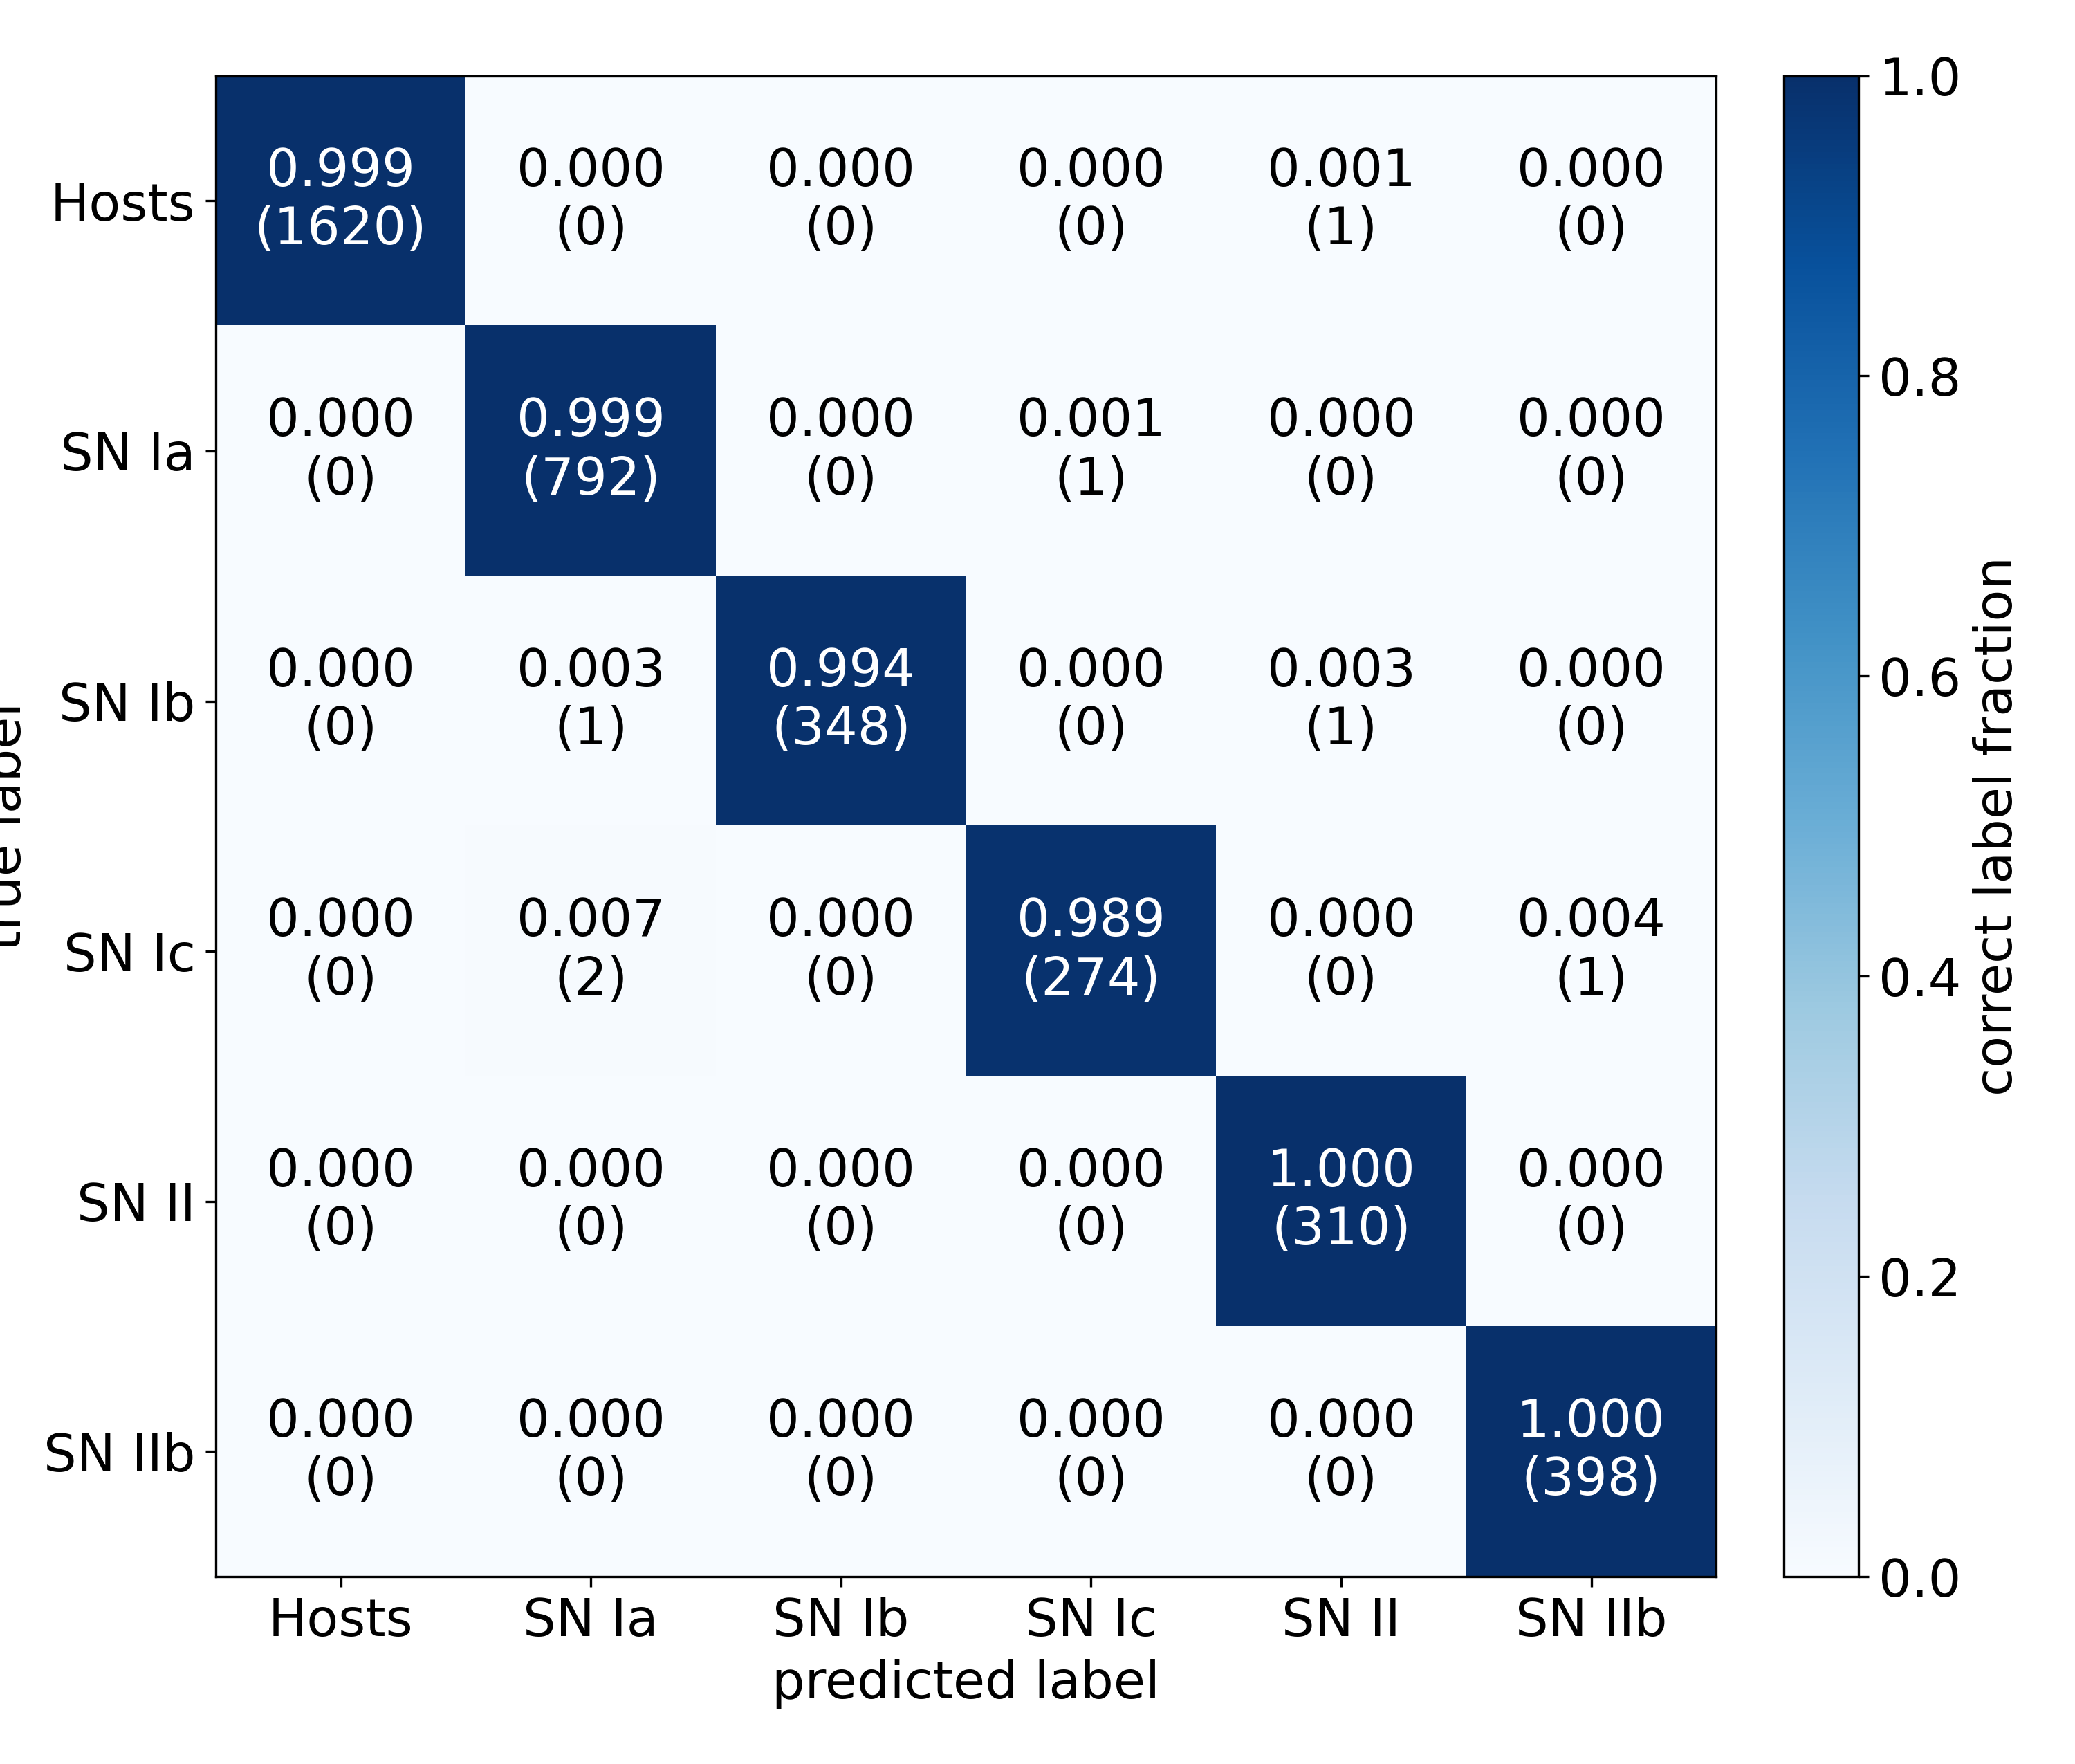
\includegraphics[height=4.55cm]{figures/cnn/cnn_cm99.png}
    \caption{CNN Diagnostics: ROC Curve (left) and Confusion Matrix (right) with a 99\% confidence cut\label{fig:cnn_qual2}}
\end{figure}

A \textbf{much better ROC curve and confusion matrix }are produced by 
evaluating the diagnostics for only highly confident classifications (Figure~\ref{fig:cnn_qual2}). 
Therefore, it is clear that the CNN, when confident in its classification, produces 
accurate results. This cut, however, is not ideal, removing *insert percent*\% of the 
data. 

The next step in training would be to either increase the confidence of the CNN 
or move to a different architecture, with the hopes of increasing not only 
the overall accuracy of the networks, but also the number of confident classifications.
% This begs the question, which is more important? The ability to classify a lot of 
% spectra with low confidence, or a few spectra with high confidence? Even if a 
% cut was made on the confidence of the classification, would the optimal solution
% yield better results under the same conditions? 

\section{Introduction of Transformers}\label{sec:transformers}
% Advantage of transformers in this field
Transformers are a relatively new architecture introduced in 2017 by \textcite{vaswani2017}
for natural language processing (NLP) tasks. The original architecture consists of 
an encoder-decoder system. The encoder accepts a series of tokens and produces a series of vectors
representing the input data via a series 
of self-attention layers and feed-forward layers. The decoder then takes the output of the encoder, and
produces a series of tokens, one for each input token. 

Once transformers were shown to have remarkable success in NLP tasks, they were 
quickly adapted to other fields, such as vision. \textcite{dosovitskiy2020} developed 
a vision transformer (ViT) architecture that differed from the original transformer 
encoder by replacing the tokenized input with a more involved preprocessing step. In short, 
the input image is broken into a series of patches, which are then flattened into
a vector. These vectors, along with positional encodings, are then fed into the
transformer architecture. For classification tasks, the first input token is 
replaced with a class token. After passing through the transformer, the class token 
is then run through a fully connected layer to produce the final probabilities. 

\subsection{ViT on Spectroscopic Data}\label{sec:ViT}
Previous implementations of transformers have been shown to have characteristics 
beneficial to the classification of spectral data. A transformer's 
ability to learn contextual information is essential in spectral classification. 
A broad absorption line, for example, may be indicative of a Type Ia supernova 
if in one part of the spectrum, but may be indicative of a Type II supernova if
in another part of the spectrum. This contextual information is not easily learned 
by a CNN, as the convolutional layers are not able to learn the importance of
certain parts of the input space. Attention can also play a role in identifying 
the purpose of features that are not in a standard location. For example, a 
\textbf{non-k corrected s}pectrum might have a continuum pattern at different locations 
in the spectrum, but the overall shape would be similar. This change in sizing 
would be difficult to learn with fixed filters in a CNN, but would be identified 
based on their positional importance by a transformer. In addition to this, ViTs 
have been shown to outperform CNNs on vision tasks, which shows they are capable 
of focusing on learned features. 


* Include caveat about the fact that ViTs take longer to train than CNNs *




% \chapter{Validity of Transformers for Spectral Classification}
% \label{chap:chapter-3}
% \section{Creation of artificial spectra}
% \label{sec:creation}
% Creating large amounts of high signal-to-noise signals was essential to verifying 
% the application of a Vision Transformer. These signals needed to include the 
% basic features of supernova spectrum, such as the presence of a continuum, 
% absorption lines, and emission lines. The locations of these spectral features 
% in particular were not important, as long as each class of supernovae had consistent 
% features. The \texttt{GenData} class was created to generate these signals. 

% \subsection{Features of \texttt{GenData} class}
% \label{ssec:features}
% The \texttt{GenData} class must provide a means of generating a large number (order of $10^5$)
% of random spectra. These spectra must exhibit a consistent continuum, variable noise, 
% and a set of spectral features that are unique to arbitrary classes. In order to 
% accomplish this, the \texttt{GenData} class must first identify a domain in which 
% to place spectral features, noise, and the continuum. The continuum is a function across
% the domain that remains consistent for all samples, and examples can be found in Fig.~\ref{fig:continuumoptions}.
% A set number of spectral features are randomly placed within the domain. The number of spectral
% features is determined by the user. Then, each class (or type) of spectra is assigned 
% a random combination of these spectral features. This is to ensure that each class 
% has a unique set of spectral features, while maintaining a consistent location of features. 
% Once the different classes are specified, the creation of the spectra can begin.

% \begin{figure}
%     \centering
%     
\includegraphics[width=0.5\textwidth]{figures/blackbox.jpeg}
%     \caption{Examples of different continuum options
%     (from left to right: linear, linear increasing, linear decreasing, 
% exponential increasing, and exponential decreasing).}
%     \label{fig:continuumoptions}
% \end{figure}

% \subsection{Creation of spectra}
% \label{ssec:creation}
% Once the spectral features present in each class are determined, the spectra can 
% be constructed from the ground up. First, the continuum is created 

% The essential Some of the features of the \texttt{GenData} class are as follows:
% \begin{itemize}
%     \item The ability to generate a large number (order of $10^5$) of random spectra
%     \item The ability to generate spectra with a continuum
%     \item The ability to generate spectra with absorption lines
%     \item The ability to generate spectra with emission lines
%     \item The ability to generate spectra with a combination of all three
%     \item The ability to generate spectra with a combination of all three, but with 
%     different spectral features in each spectrum

% \end{itemize}
\chapter{Creation and Training of Spectral ViT}
\label{chap:methods}
% Methods to validate transformers (fake spectra), create training data (fake spectra), 
% train various models (V1.1, V1.2, V1.3, V2), to find optimal training for V2

In order to examine the effectiveness of the transformer architecture for supernovae
spectral classification, a series of steps were taken. First, an in-house transformer 
architecture was created based on the traditional ViT architecture \cite{dosovitskiy2020}, 
which was quickly found to be trainable on a synthetic dataset. Next, a synthetic dataset 
using DESI spectra was created under a variety of preprocessing conditions. The previously 
created CNN and new transformer architectures were trained on each variation of 
preprocessed data. Finally, these training sessions were then used to determine 
the optimal training conditions for non red-shift corrected data. 
\section{Creation of Spectral ViT}\label{sec:SpecViT}
The Spectral ViT architecture was created to be a direct extension of the ViT architecture
\cite{dosovitskiy2020} to be used for spectral classification, coded in the \texttt{PyTorch}
deep learning framework. The Spectral ViT architecture is shown graphically in
Appendix~\ref{app:SpecViT}. The Spectral ViT architecture is
composed of three main components: the pre-processor, the encoder, and the classifier. 

The pre-processing component is responsible for taking the (already preprocessed)
input spectra and converting it into a series of vectors that the transformer can interpret. 
Considering a group of $N$ spectra, each with $10000$ pixels, the each group 
is split into a set number of patches (approximately 100). Each patch is then 
linearly mapped via a fully connected network to a vector three times the patch size.
The sample is now a set of of size $N\times101\times300$. 
A classification token of the sample dimensionality as the patches 
is then added to the beginning of each sample, initialized randomly. 
In order for the transformer to properly understand the positional relationship between each patch, an embedding 
is added to each patch. This embedding is a scalar function based on the size 
of the patch is calculated as follows: 
\begin{equation}
    \text{Embedding}_{ij} = \begin{cases} \sin\left(\frac{i}{10000^{(j / \text{patch size})}}\right) & \text{if } j \text{ is even} \\
    \cos\left(\frac{i}{10000^{((j - 1) / \text{patch size})}}\right) & \text{if } j \text{ is odd}\end{cases},
\end{equation}
where $i$ is the position of the patch in the vector, and $j$ is the position of the patch in the sample~\cite{vaswani2017}.
A visual representation of the embeddings for the sample is shown in Fig.~\ref{fig:embedding}. Once the 
embeddings are added element-wise to the patches, the resulting tensor (of size $N\times101\times300$) is then passed through the encoder. 
\begin{figure}[H]
    \centering
    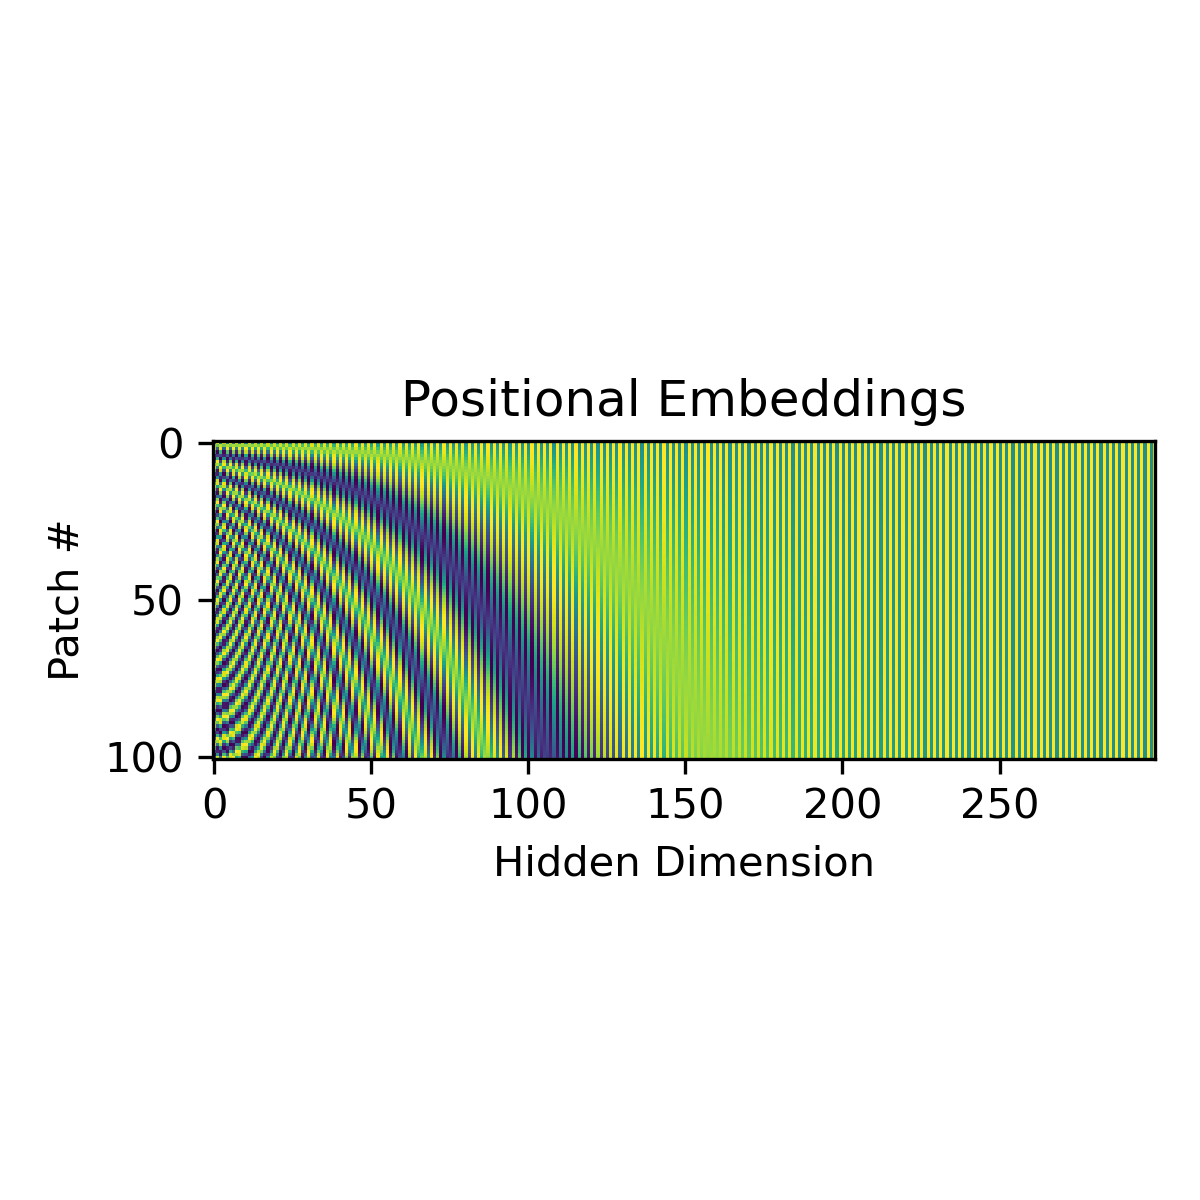
\includegraphics[width=.4\linewidth]{figures/embeddings.png}
    \caption{Visual representation of the embeddings for a sample of spectra split into 100 patches of length 300.}
    \label{fig:embedding}
\end{figure}

The encoder is the main component of any ViT architecture, as it contains the 
multi-head attention and feed-forward layers. The encoder is composed of a set number of
transformer blocks, each of which contains layer normalization, multi-head attention, another 
layer normalization, and finally a feed-forward layer. The multi-head attention layer 
is a scaled dot-product attention layer found in \textcite{vaswani2017}. Each patch 
is passed through three separate linear layers, each with a different set of weights, 
resulting in three sets of vectors: the query ($Q$), key ($K$), and value ($V$).
\begin{equation}
    \label{eq:mhsa}
    \text{Attention}(Q, K, V) = \text{softmax}\left(\frac{Q\cdot K^T}{\sqrt{d_k}}\right)\cdot V
\end{equation}
The dot-product between the query and key vectors is then calculated,
scaled by the square root of the dimensionality of the query vector, and then passed through a softmax function.
The resulting attention weights are then multiplied by the value vectors (Equation~\ref{eq:mhsa}). 
This is simultaneously done for each head in the multi-head attention layer. Each result is then 
concatenated together, and then passed through a linear layer to reduce the dimensionality
to the size of the query vector. This resulting vector is then added
element-wise to the original patches, normalized, and then passed through a MLP, 
resulting in a tensor of size $N \times 101 \times 300$. This again is added element-wise to the original patches. 
Each step is repeated for a set number of transformer blocks, resulting in a tensor of size
$N \times 101 \times 300$.

The final component of the Spectral ViT architecture is the classifier. The classifier
takes in only the first patch of each sample, which has been designated as the classification token.
The classification token is passed through a linear layer to reduce the dimensionality to the
number of classes, and then passed through a softmax function to produce a probability distribution
over the classes. Therefore, the resulting tensor is of size $N \times 1 \times 6$, for our 
6 classifications of supernovae.
\subsection{Validation of Spectral ViT Architecture}
\label{ssec:validation}
After the creation of the Spectral ViT architecture, ability to train effectively 
was tested. A synthetic dataset, consisting of a consistent continuum with 
Gaussian peaks placed at preditermined locations, was created. Certain combinations of 
peak locations were chosen to represent an arbitrary `class' of supernovae. These peaks, 
our synthetic emission lines, were given random amplitudes and widths, simulating  
variability, with a maximum allowed value. This maximum allowed value was then used to add 
Gaussian noise to the signal: either 2 or 5 times the signal to simulate noisy ($S/N=2$),
or very good data ($S/N=5$). Examples of the synthetic spectra with different continuum profiles 
are shown in Fig.~\ref{fig:synth_spectra}. 

These datasets with a signal-to-noise of 5 trivially separable by a smaller Spectral ViT architecture, 
which was able to achieve 100\% accuracy on the testing set. The lower quality data, however, 
was more difficult to separate, only achieving an 82\% test accuracy.

** PUT IN GRAPHS OF SYNTHETIC SPECTRA HERE **
** PUT IN GRAPHS OF TRAINING SYNTHETIC SPECTRA HERE **
** PUT IN TABLE OF TRAINING SYNTHETIC SPECTRA HERE - SN=2 and SN=5**

\section{Creation of Synthetic DESI Spectra}
\label{sec:synth_data}
Once the Spectral ViT architecture was shown to be able to train effectively on synthetic data,
the architecture was ready to be trained on DESI data. In order to create a large enough training 
set, authentic DESI spectra were used as a base to create synthetic spectra.

** Talk to BenZvi about what to put in this section / who to cite for all of the work **

\subsection{PreProcessing of DESI Spectra}
\label{ssec:preprocess}
% All of preprocessing including z correction and downsampling 
Once the spectra's were created and saved as DESI files, they needed to be 
extracted, preprocessed, split into training, testing, and validation sets, 
only then could they be saved, and used to train the Spectral ViT architecture.
The preprocessing method developed by ** Cite eddies paper **, and is split into 
3 main steps: z correction, rebinning / down sampling, and normalization. 

The Z correction step was used to move the spectra back into the rest frame using 
the redshift fitted to the original spectra by the DESI pipeline. Next, all artifacts 
in the spectra (masks, bad pixels, etc.) were removed. The spectra were then re-binned
and downsampled to a variable resolution (default 3600). Afterwards, the spectra were 
normalized by moving the max and min values to 1 and 0 respectively. Finally, for the 
CNN datasets, the spectra were split into a 2D array of equal height and width. 
After this, the spectra were split into training, testing and validation datasets that 
comprised of 60\%, 20\%, and 20\% of the total dataset, respectively.
\section{Training of Neural Networks}
\label{sec:training} 

\subsection{CNN Training}
\label{ssec:cnn_training}
CNN training was conducted using DESI spectra downsampled to a resolution of 3600, and 
put into a 2D array of equal height and width. The CNN architecture was developed 
by ** Cite eddies paper **, and has properties shown in Table~\ref{tab:cnn_architecture}.
This CNN was trained for a maximum of 50 epochs, with a batch size of 50, and 
non-variable hyperparameters (Table~\ref{tab:cnn_hyperparameters}). 
The timeline of the training of the CNN architecture is shown in Fig.~\ref{fig:cnn_training}.


\subsection{Transformer Training}
\label{sec:transformer_training}
The Spectral ViT architecture, idealistically, should have the capability to be trained 
on non rest-frame corrected spectra. In an effort to test how down-sampling had 
affected the training of the Spectral ViT architecture, the Spectral ViT architecture
was trained on various downsampling values. Based on these models, a downsampling 
value was chosen for non-rest-frame corrected spectra. The Spectral ViT architecture 
was trained on DESI spectra downsampled to a resolution of 3600, 1800, and 900. 
The Spectral ViT architecture was trained for a maximum of 100 epochs, with 
batch sizes of 50, and non-variable hyperparameters (Table~\ref{tab:transformer_hyperparameters}).



\chapter{Spectral ViT Model Performance}
\label{chap:results}

\section{Spectral ViT V1: A suitable replacement}\label{sec:v1_results}
The Spectral ViT's performance was evaluated on the test set of 12888 validation spectra.
These spectra were not used in the training, nor the test set of the model. The resulting 
ROC curve and confusion matrix are shown in Figure~\ref{fig:v1_qual}. The ROC curve 
shows the model is capable of differentiating between SNe and non-SNe with an AUC of 0.99.
However, differentiating between the different types of SNe is more difficult, as the
confusion matrix indicates. 
\begin{figure}
    \centering
    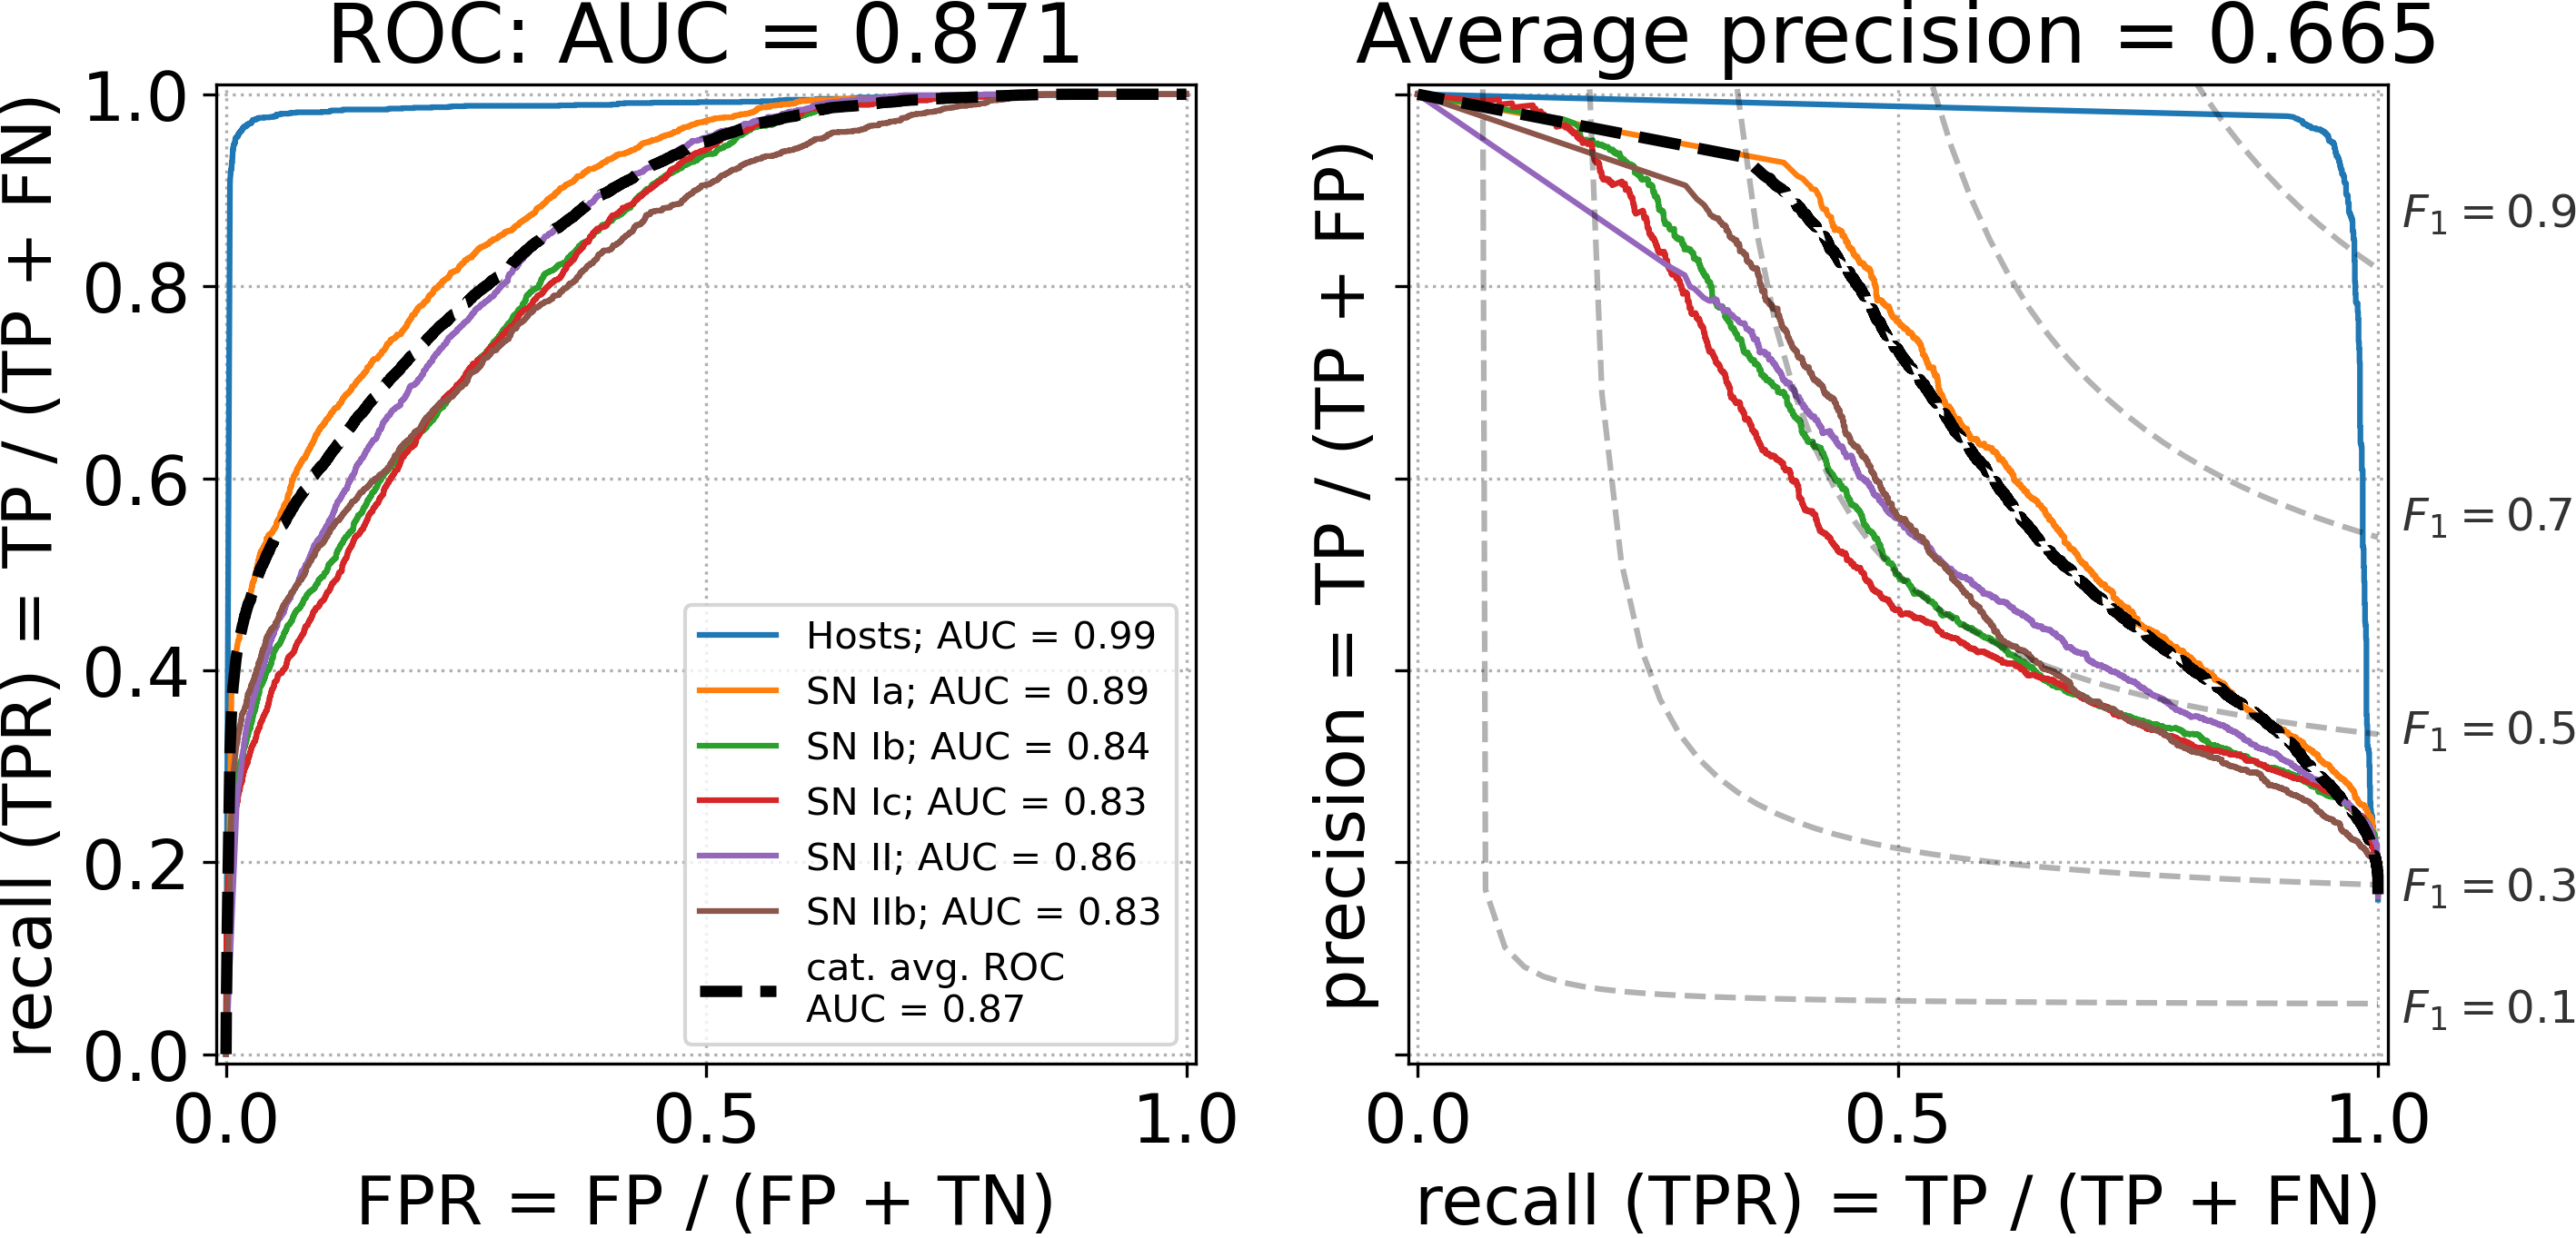
\includegraphics[height=4.3cm]{figures/v1_real/vit_model_V1_original_redorocfulle_e31.png}
    \quad
    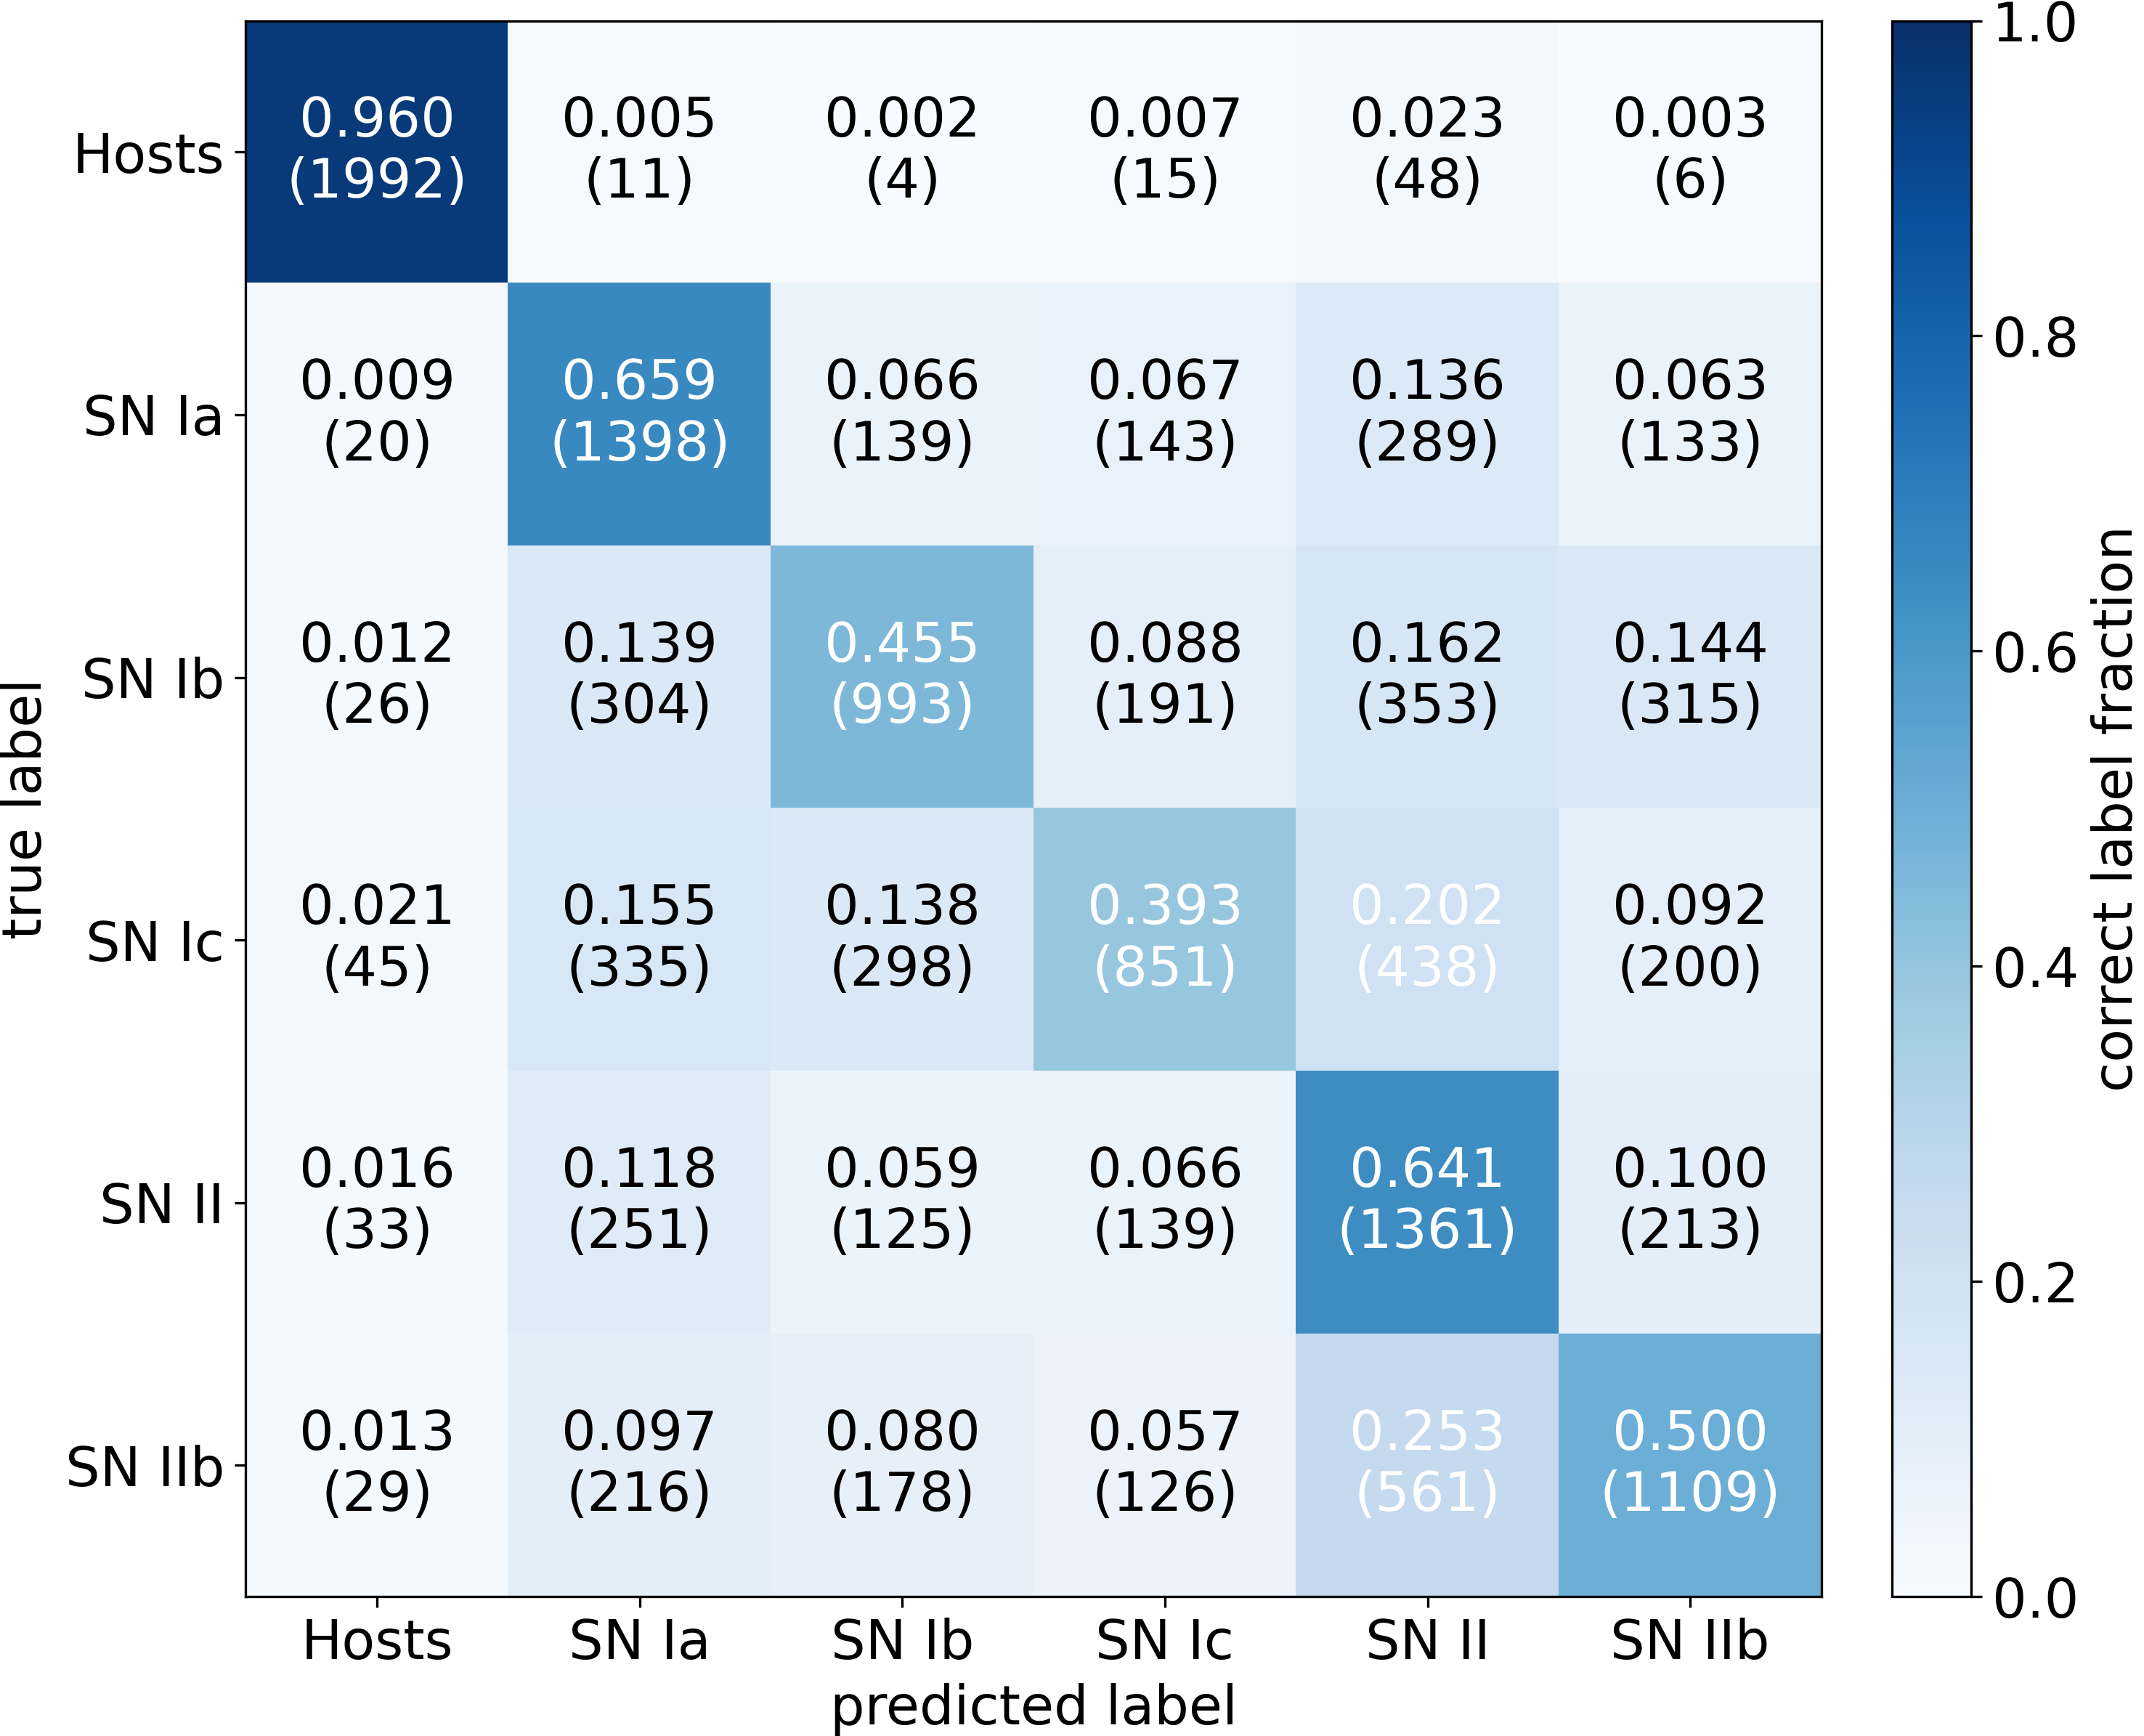
\includegraphics[height=4.3cm]{figures/v1_real/vit_model_V1_original_redocmfull_e31.png}
    \caption[Spectral ViT V1 Diagnostics]{Spectral ViT V1 Diagnostics: ROC Curve (left) and Confusion Matrix (right)\label{fig:v1_qual}}
\end{figure}

In contrast to the CNN previously used by \textcite{Sepeku2022}, the Spectral ViT V1 
was more sure of its predictions, as indicated by Figure~\ref{fig:v1_max}. By filtering 
out predictions with a maximum value less than 99\%, the model's average precision 
was increased from 0.665 to 0.783 (Figure~\ref{fig:v1_99_qual}). This cut included 
63.4\% of the original predictions. Further increasing this cut to 99.9999\% reduced 
the sample size to 5156 (40\% of the original validation size), but further increased the 
average precision to 86.2\%, as shown in Figure~\ref{fig:v1_999999_qual}.  
\begin{figure}[t]
    \centering
    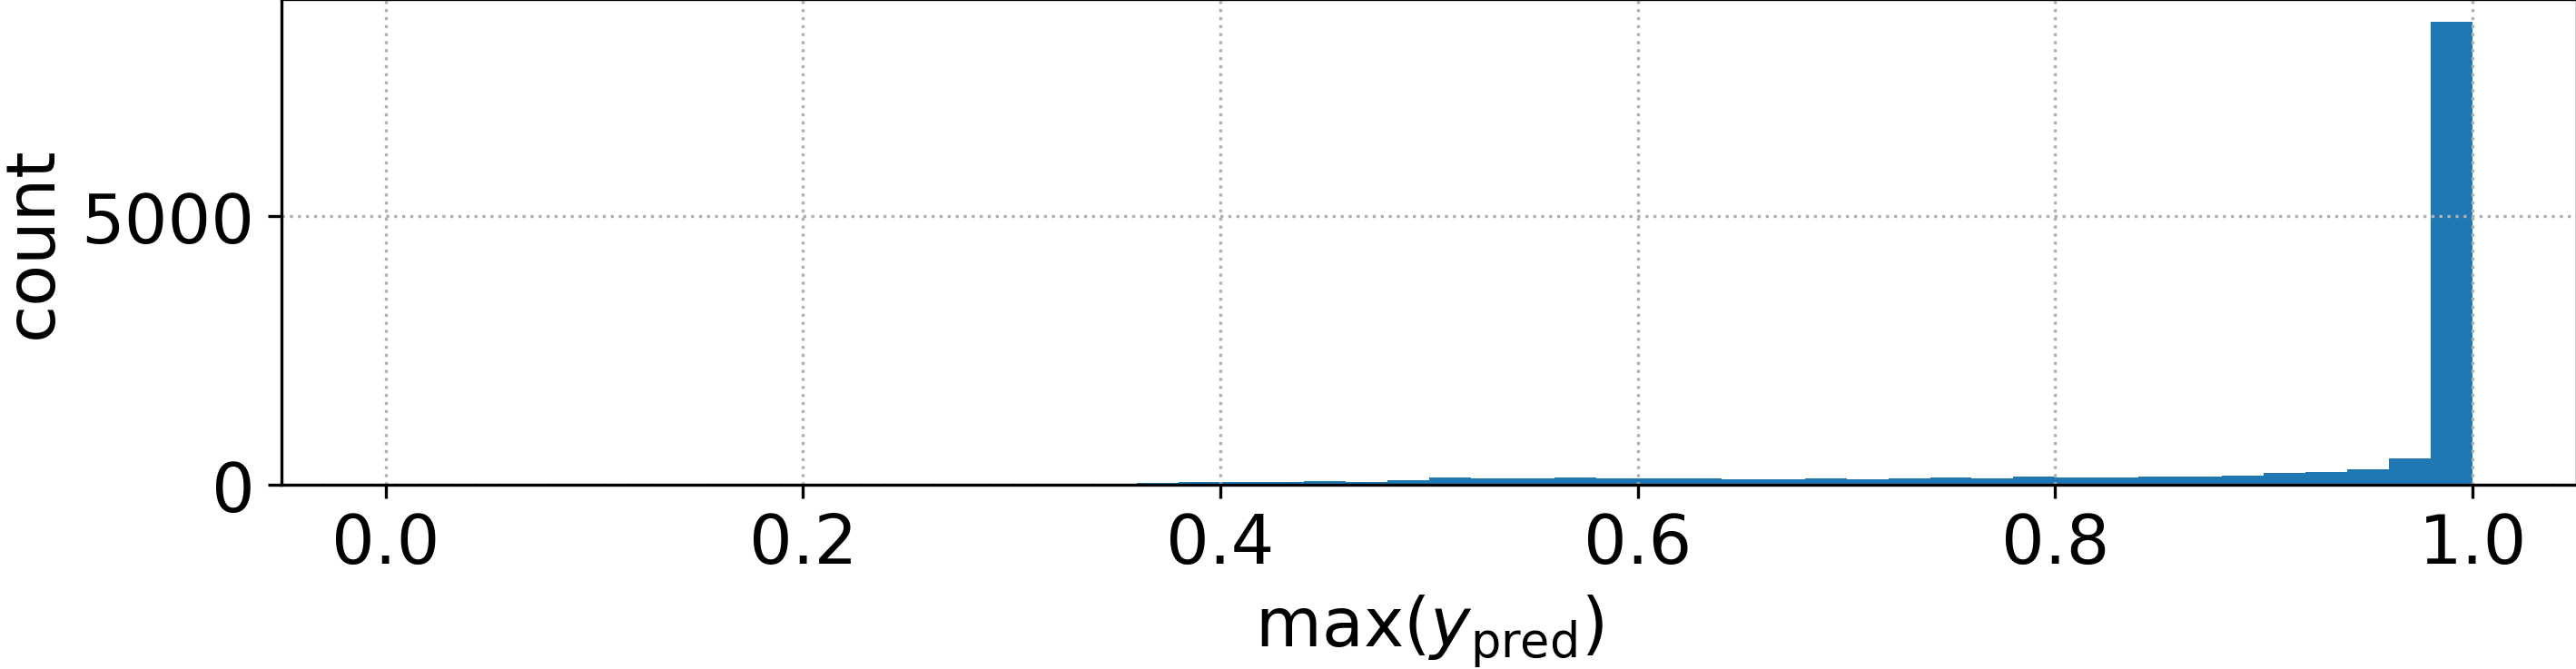
\includegraphics[width=0.8\textwidth]{figures/v1_real/vit_model_V1_original_redomax_ypred_binary_31.png}
    \caption[Spectral ViT V1 Confidence]{Max value of the output vector from the Spectral ViT V1.\label{fig:v1_max}}
\end{figure}

\begin{figure}[b]
    \centering
    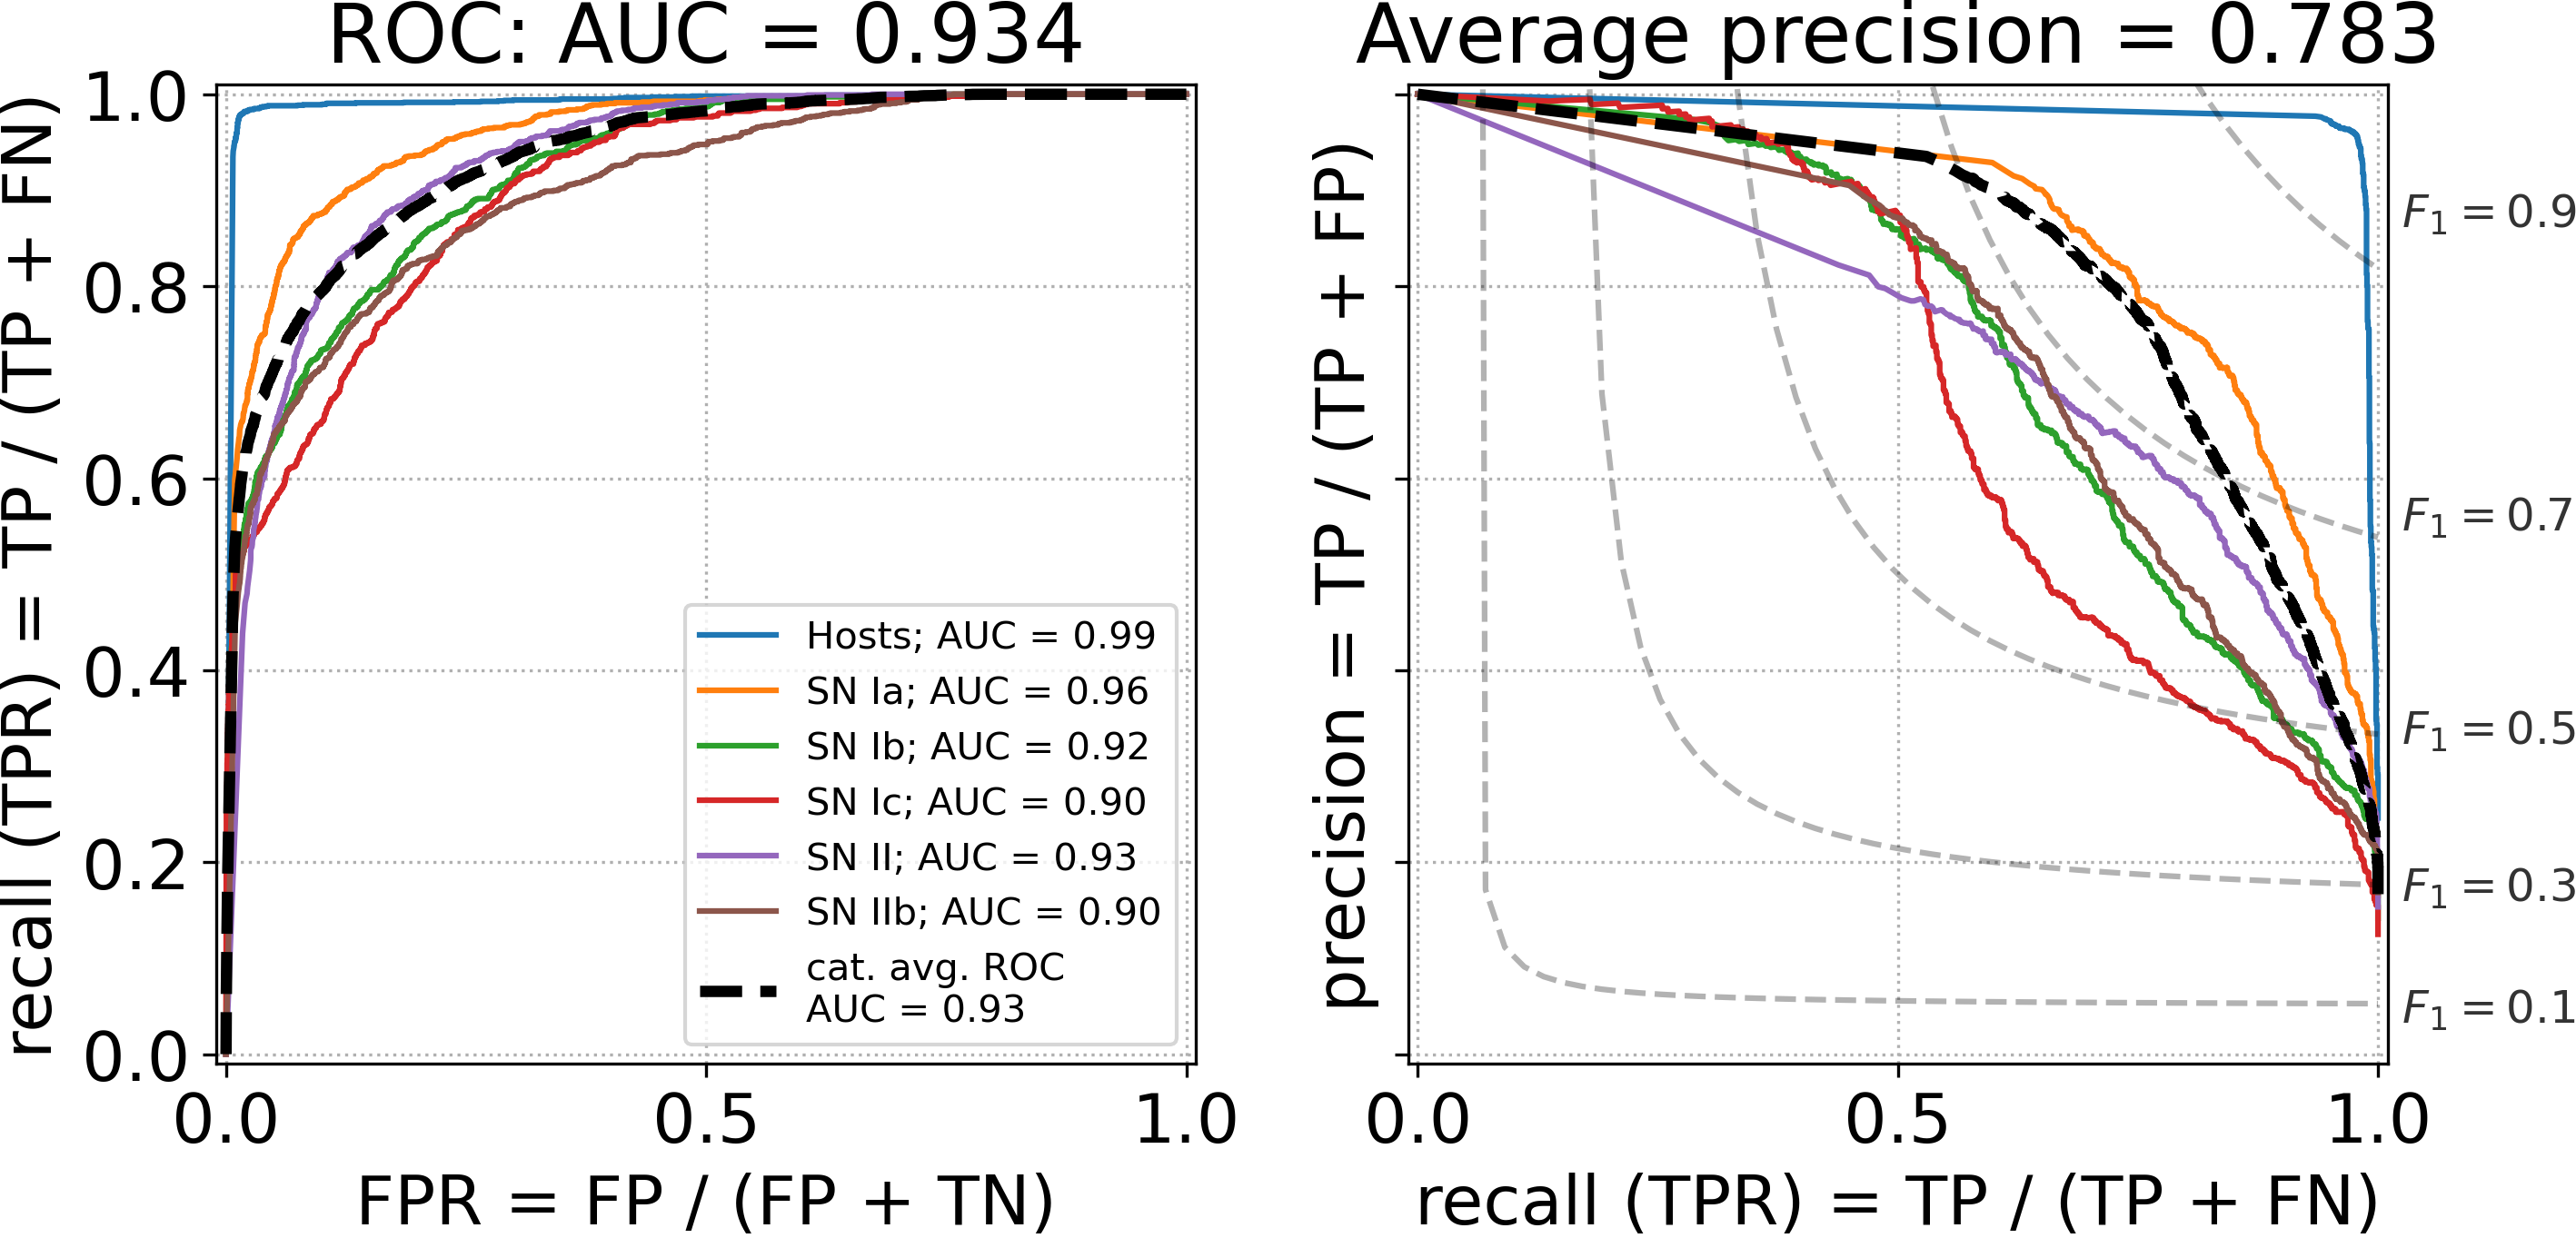
\includegraphics[height=4.3cm]{figures/v1_real/vit_model_V1_original_redoroc99_e31.png}
    \quad
    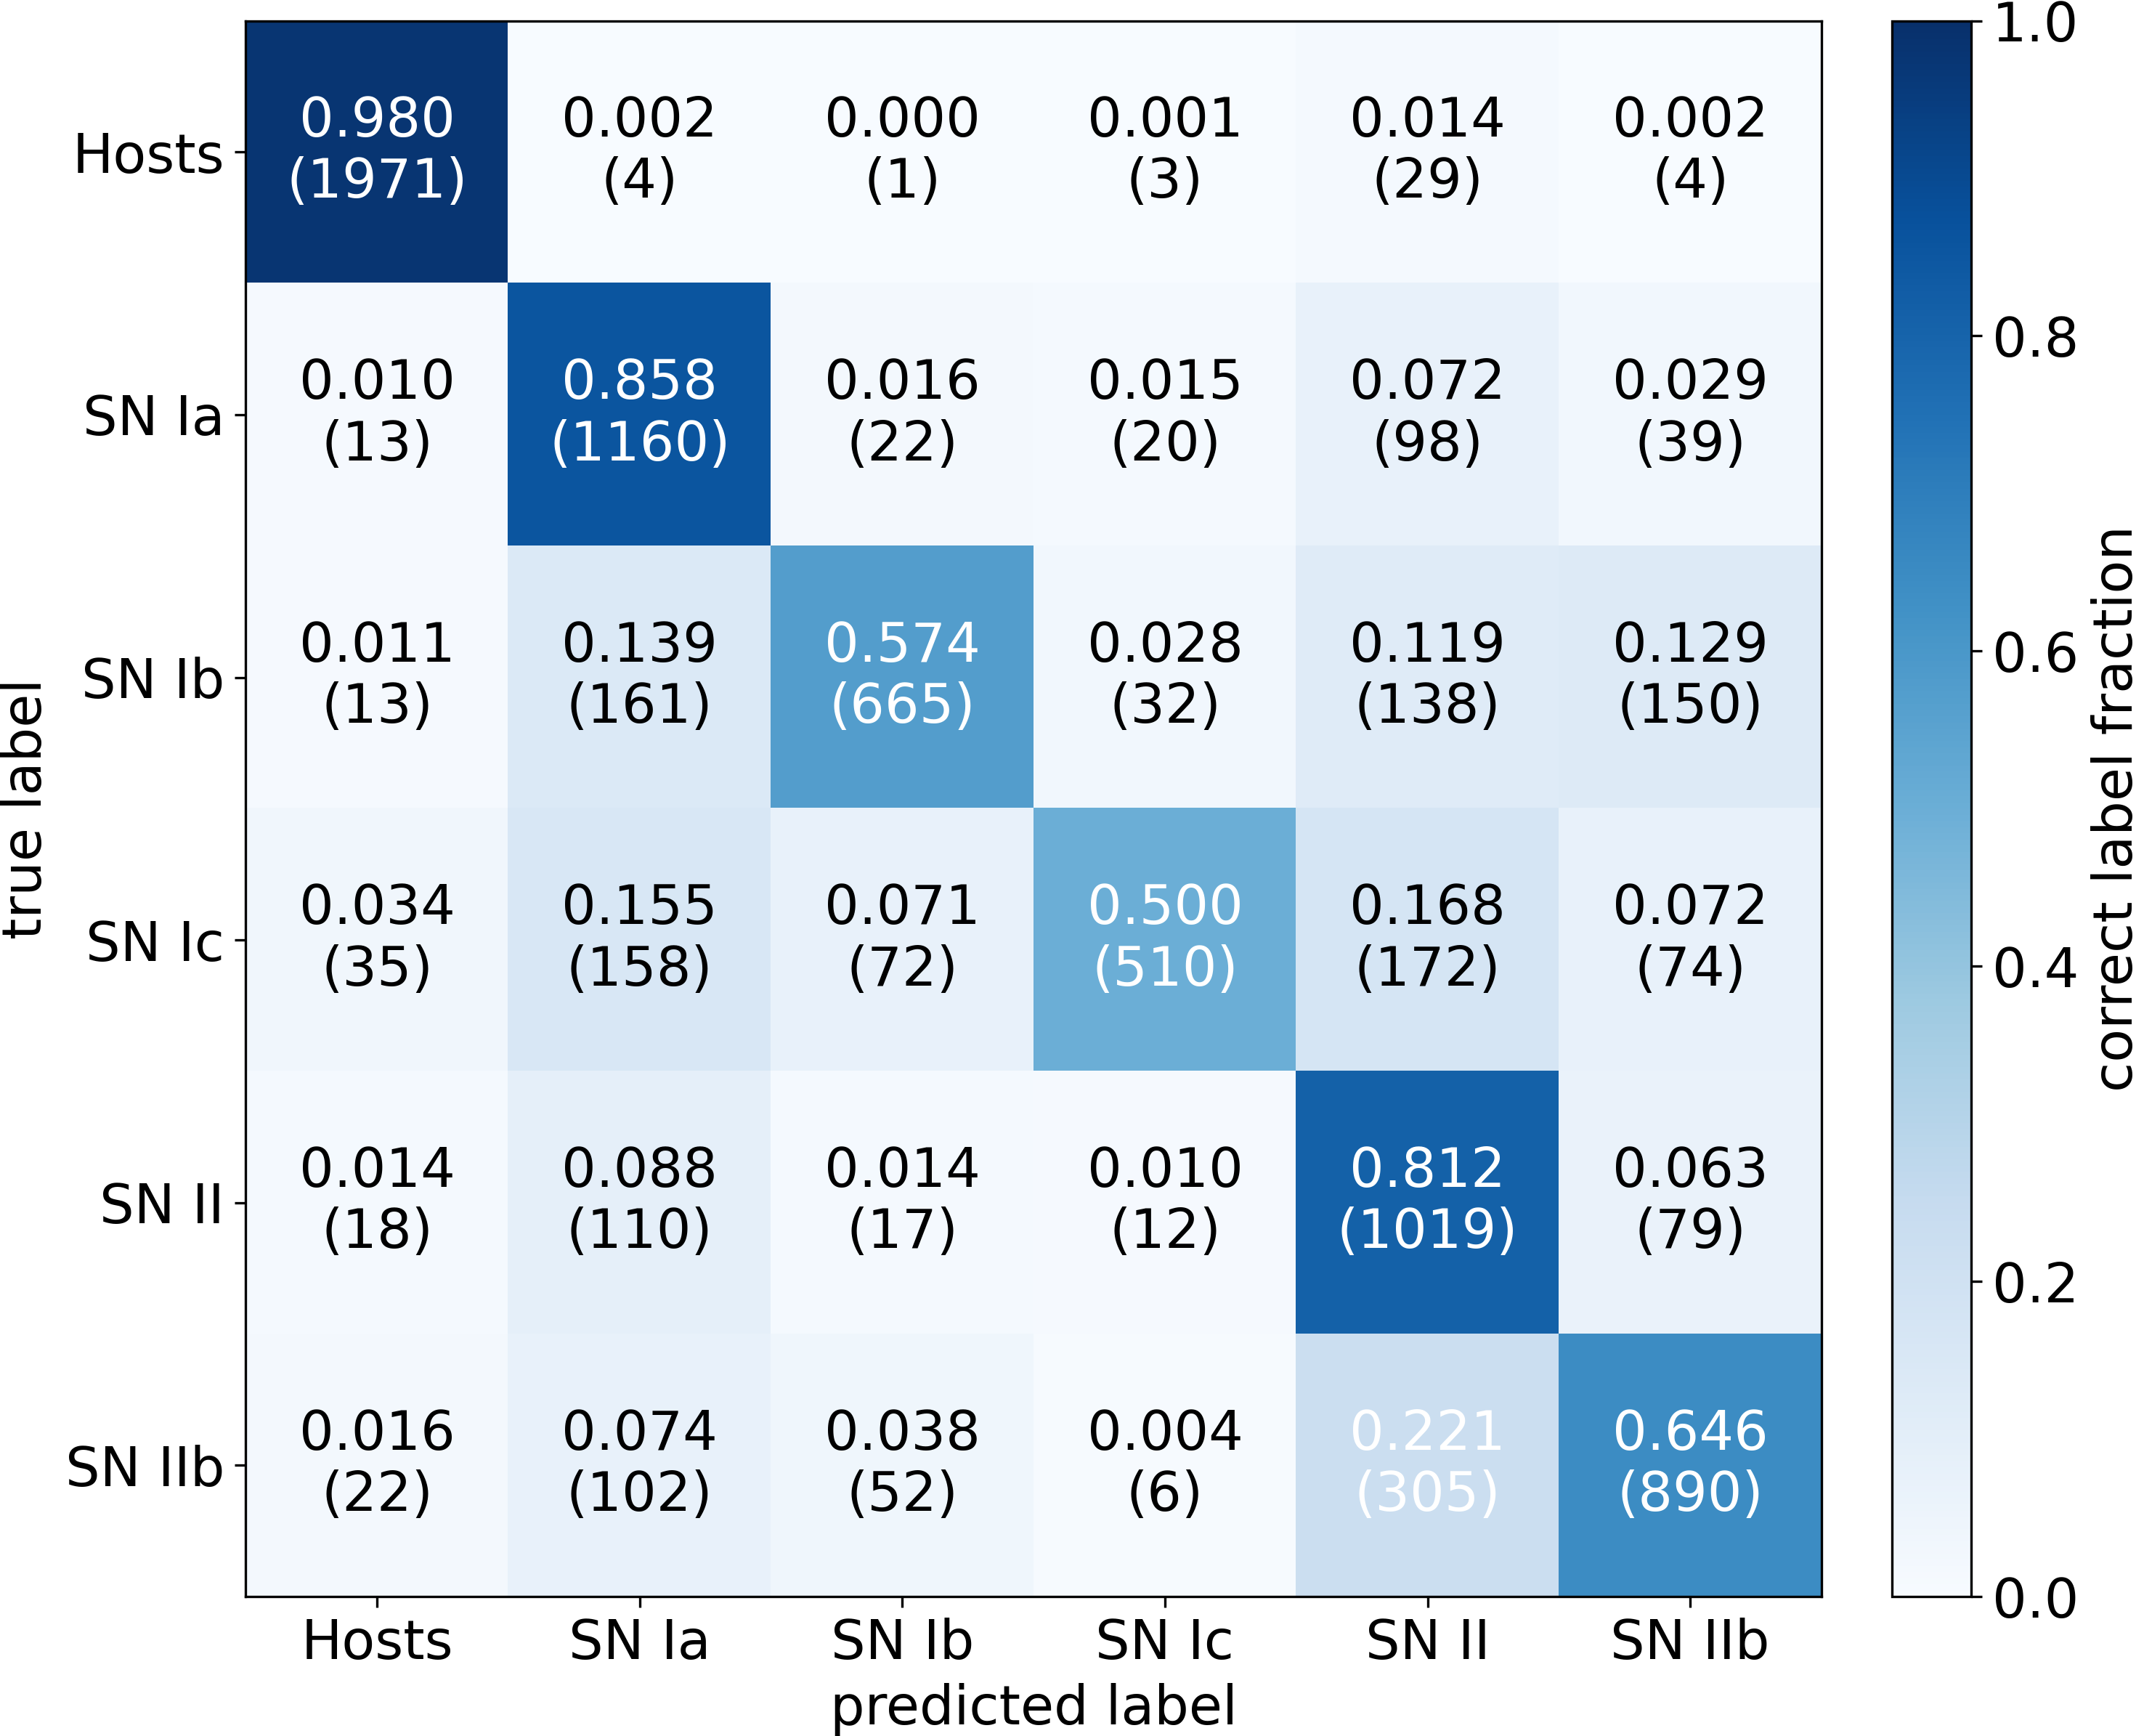
\includegraphics[height=4.3cm]{figures/v1_real/vit_model_V1_original_redocm99_e31.png}
    \caption[Spectral ViT V1 Diagnostics: 99\% Cut]{Spectral ViT V1 Diagnostics: ROC Curve (left) and Confusion Matrix (right) with a 99\% confidence
    cut \label{fig:v1_99_qual}}
\end{figure}

While the accuracy score didn't increase significantly with the second confidence cut, 
the important metric is the number of positive predictions made. All AUC scores 
are above 0.95, and the number of found targets is significantly higher than the 
CNN previously used. For example, Figure~\ref{fig:v1_999999_qual} correctly 
classifies 4705 targets, while Figure~\ref{fig:cnn_qual2} only correctly classifies 
3742 targets under a less strict confidence cut. This is a 26\% increase in the
number of correctly classified targets not excluded by the confidence cut.

\begin{figure}
    \centering
    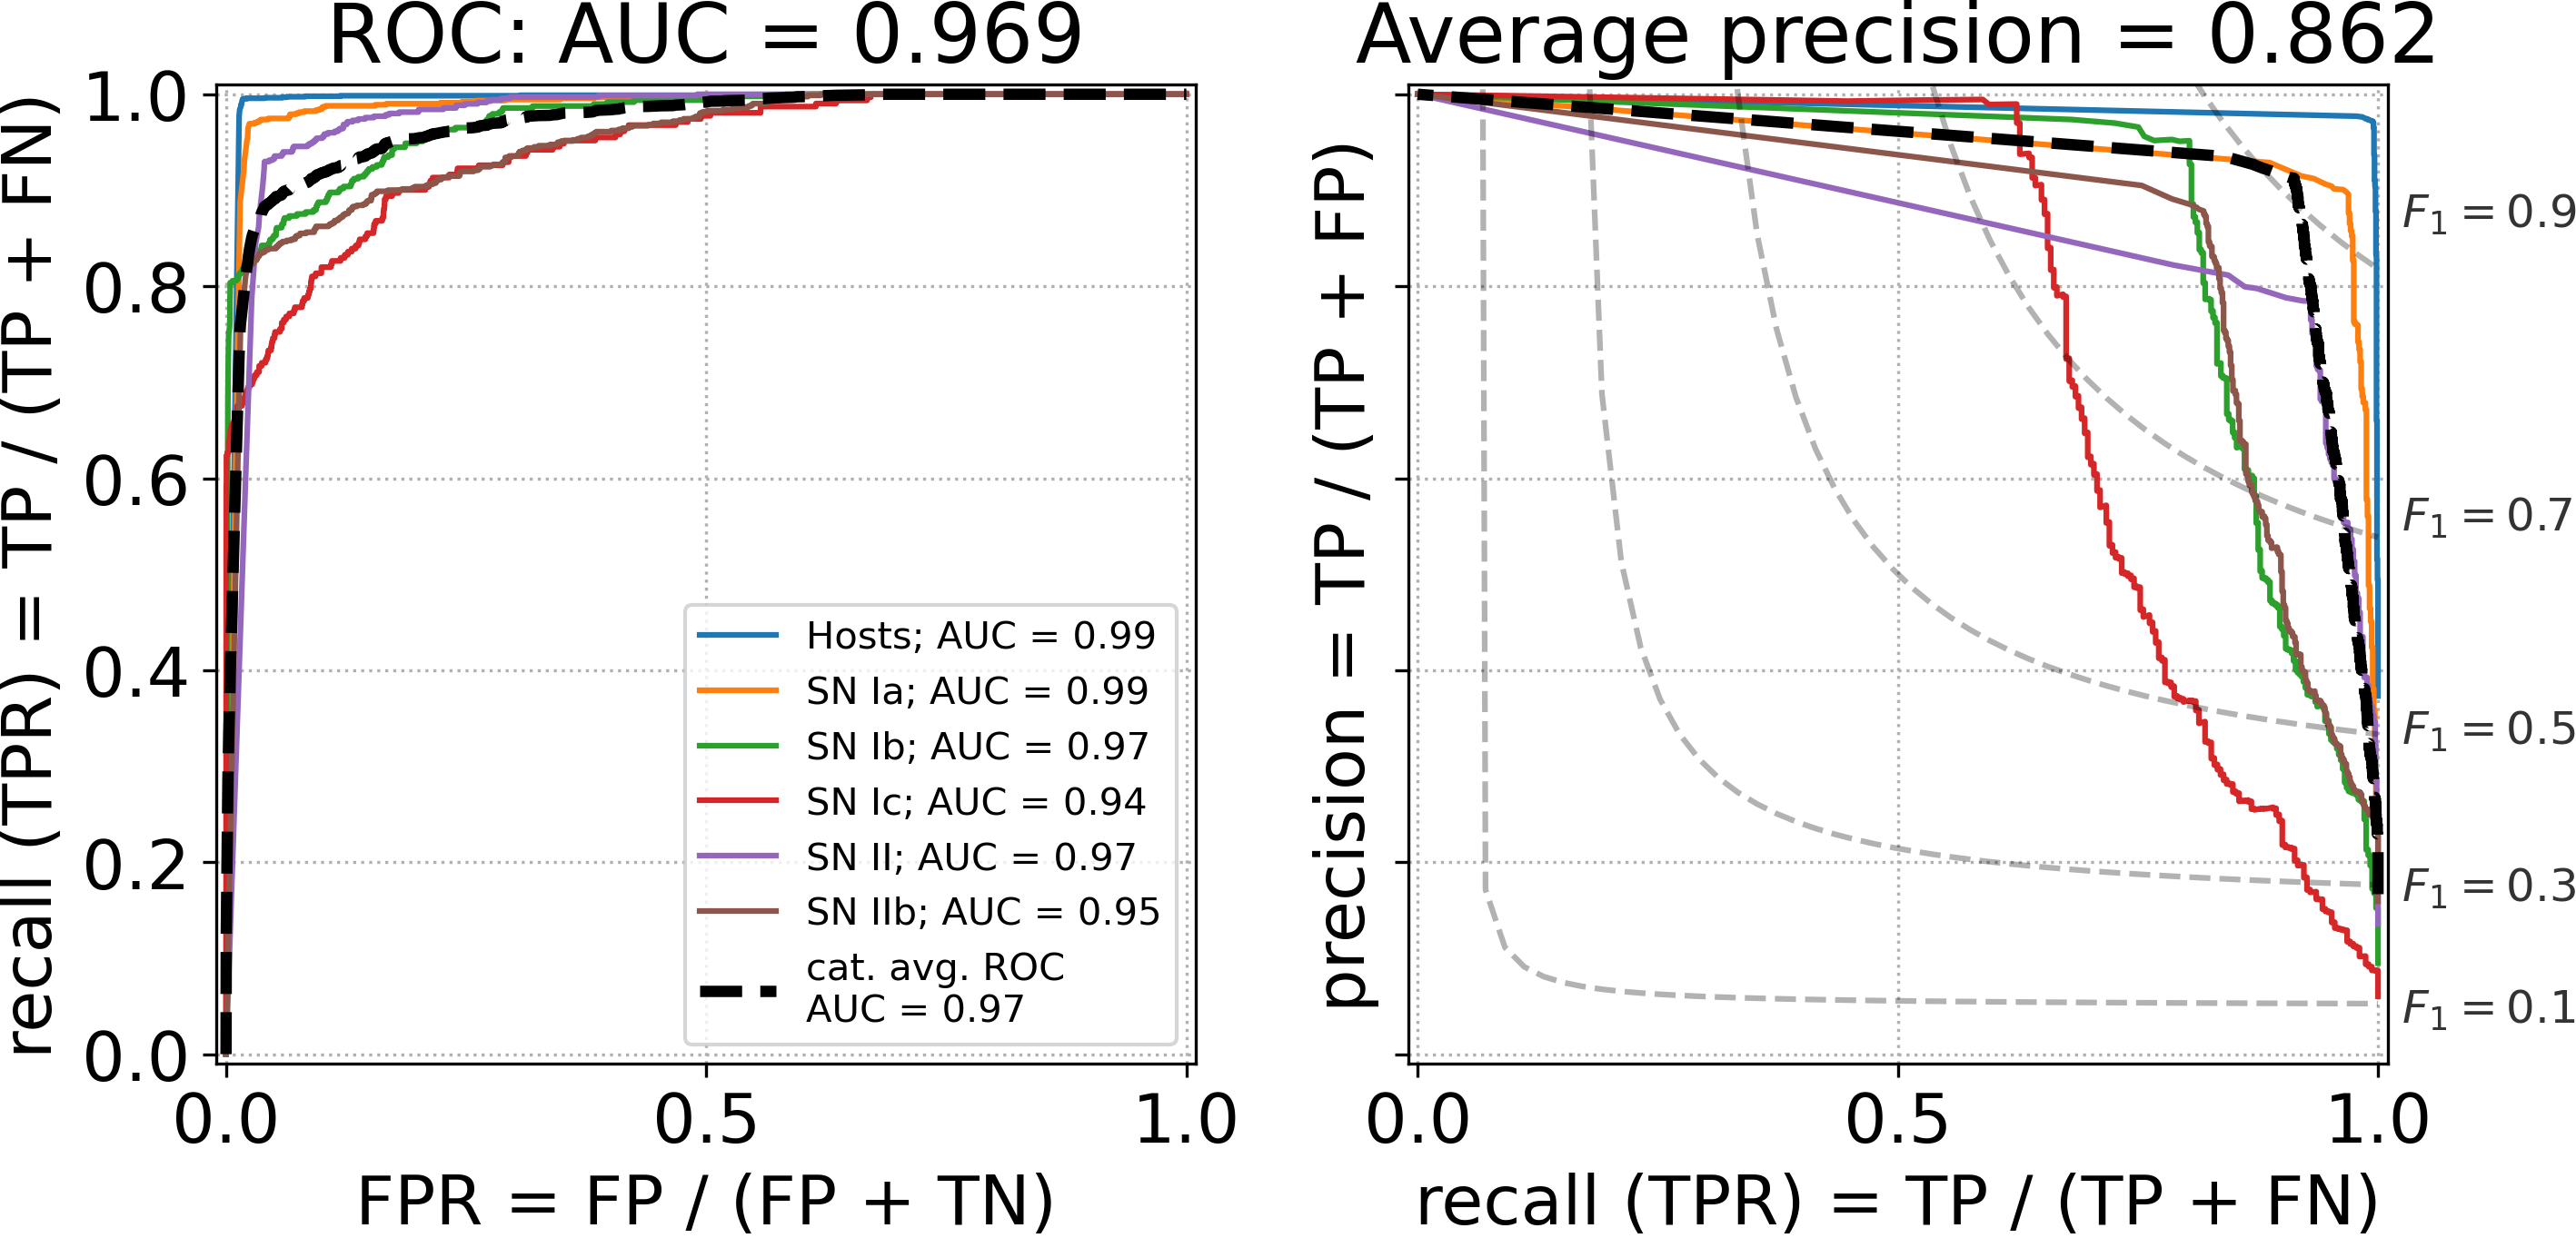
\includegraphics[height=4.3cm]{figures/v1_real/vit_model_V1_original_redoroc999999_e31.png}
    \quad
    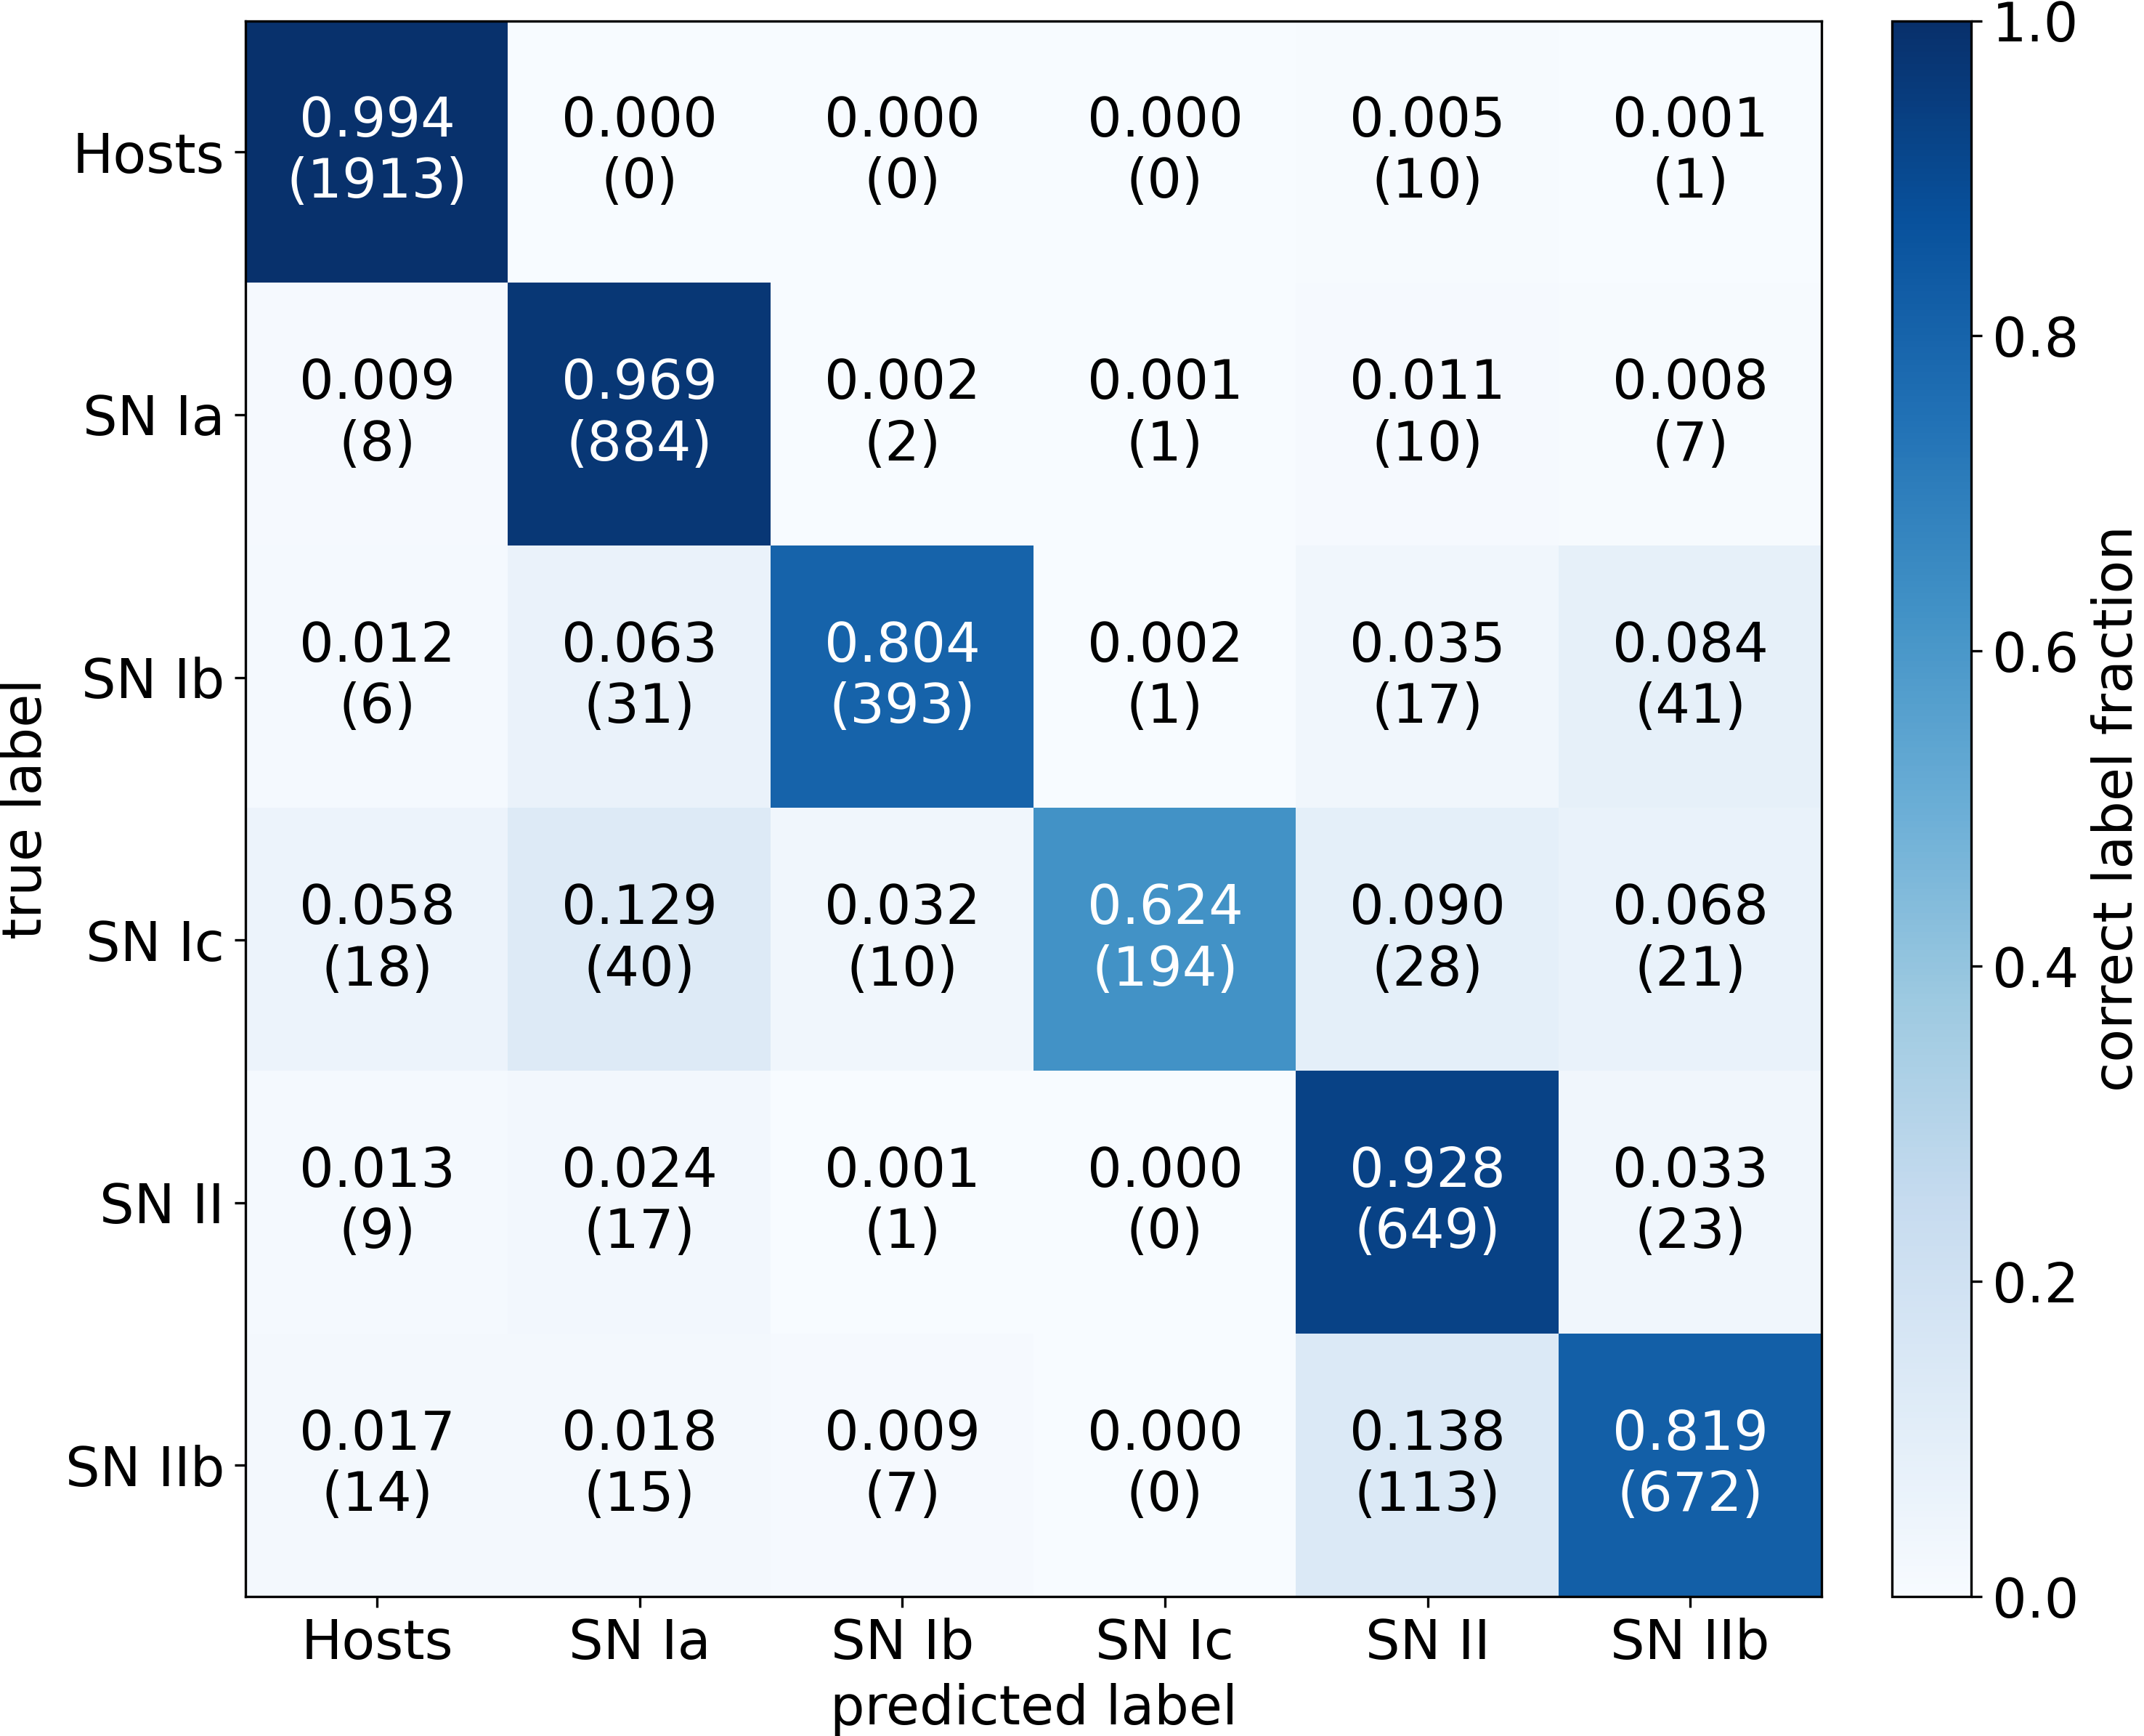
\includegraphics[height=4.3cm]{figures/v1_real/vit_model_V1_original_redocm999999_e31.png}
    \caption[Spectral ViT V1 Diagnostics: 99.9999\% Cut]{Spectral ViT V1 Diagnostics: ROC Curve (left) and Confusion Matrix (right) with a 99.9999\% confidence
    cut \label{fig:v1_999999_qual}}
\end{figure}

% \clearpage
\section{Spectral ViT V2: Specialized Classifier}
\begin{figure}[b!]
    \centering
    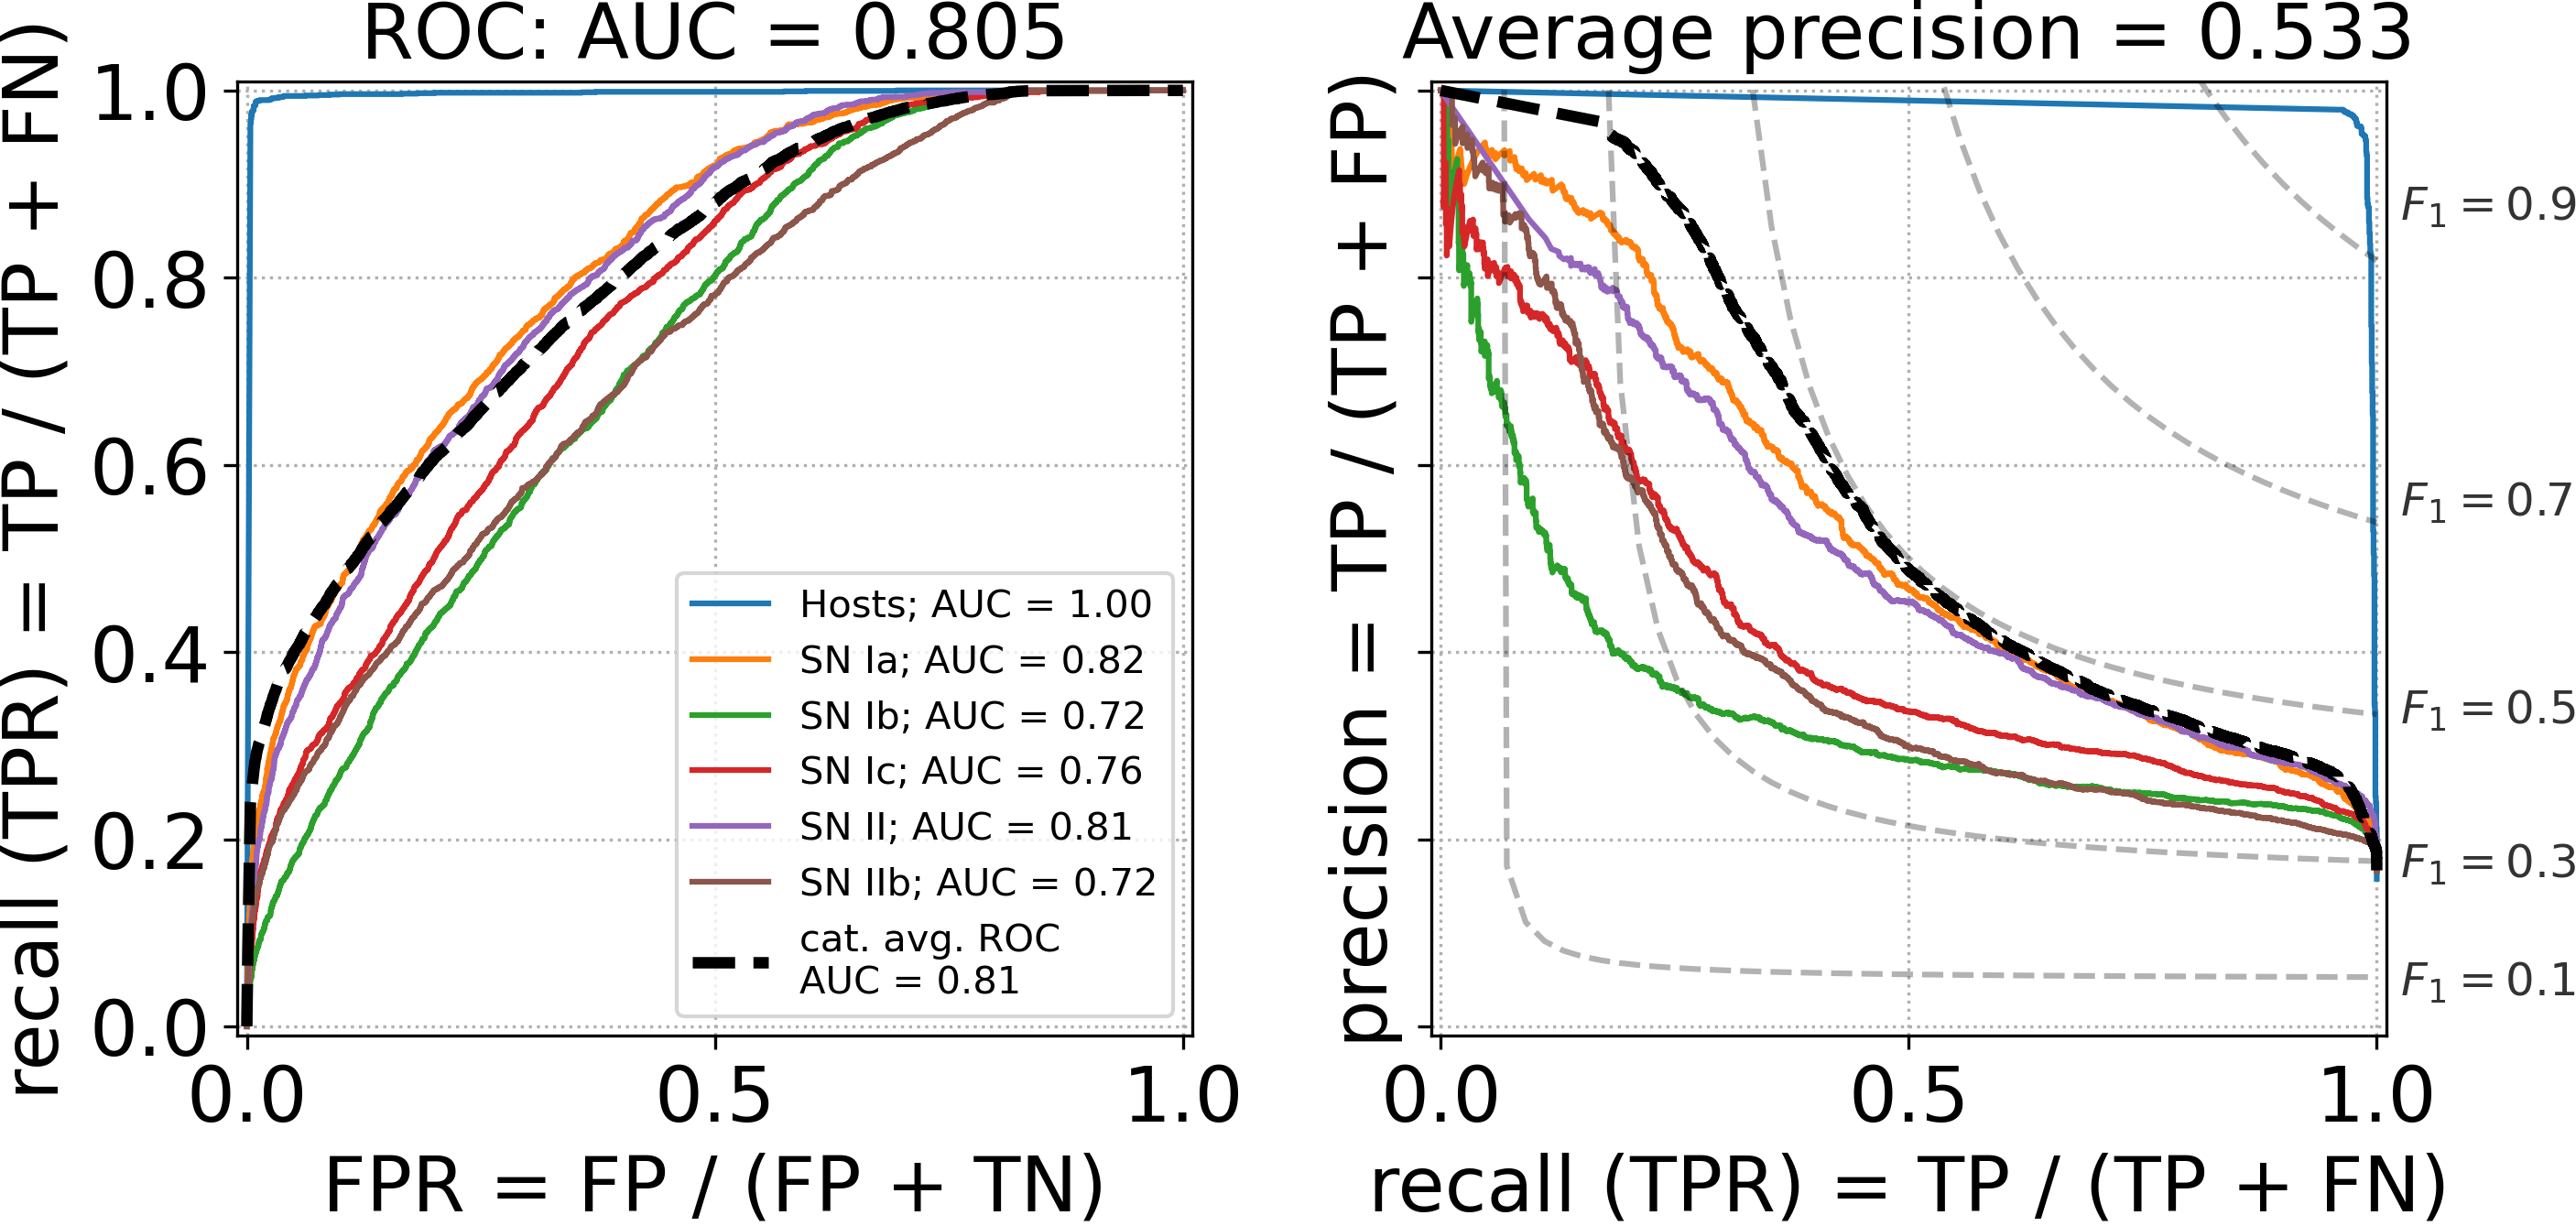
\includegraphics[height=4.3cm]{figures/v2_real/vit_model_V2rocfulle_e26.png}
    \quad
    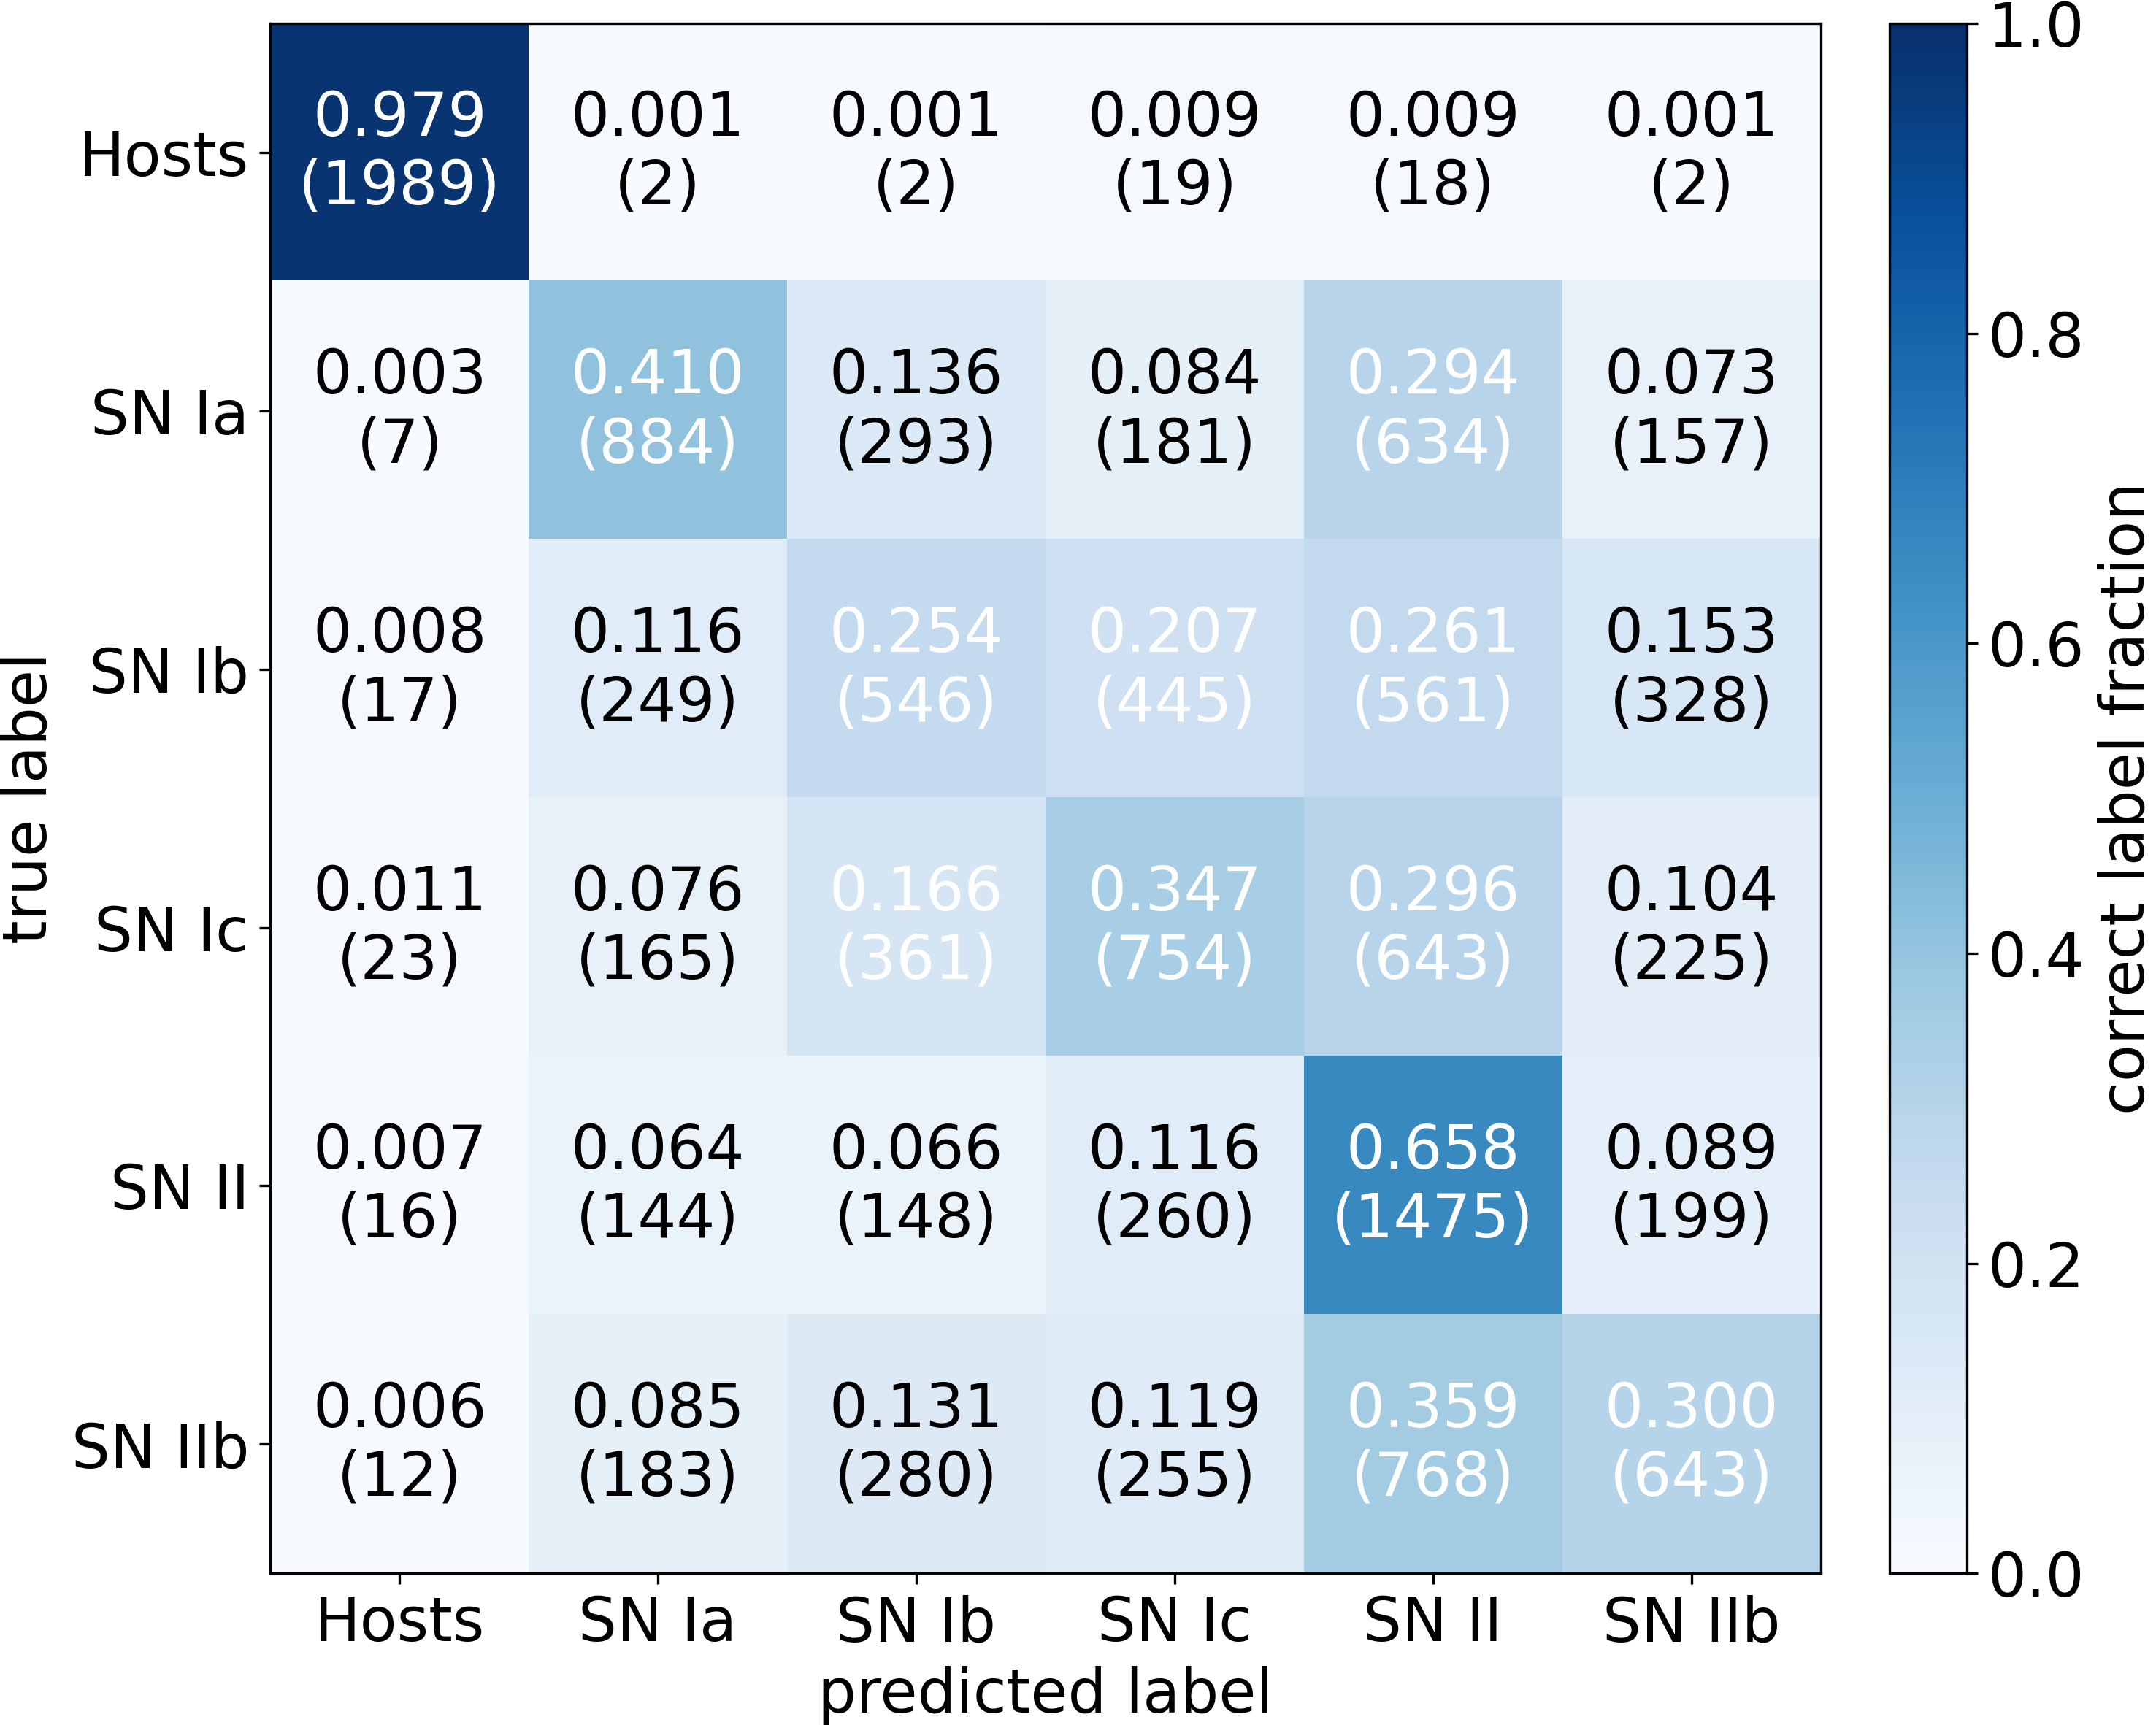
\includegraphics[height=4.3cm]{figures/v2_real/vit_model_V2cmfull_e26.png}
    \caption[Spectral ViT V2 Diagnostics]{Spectral ViT V2 Diagnostics: ROC Curve (left) and Confusion Matrix (right)\label{fig:v2_qual}}
\end{figure}
The goal of the Spectral ViT V2 was to see if the dependence on the redshift fit 
provided by the DESI pipeline could be removed. The validation set was the same size 
as the V1 validation set, 12888 specra. The ROC curve and confusion matrix are shown
in Figure~\ref{fig:v2_qual}. Classification of SNe and non-SNe is still very good,
with an AUC of 1.0, but the other classes are not classified as well, resulting in 
an overall AUC of 0.805 and a lower average precision of 53.3\%. 


Similar to the CNN, on a 99\% confidence cut, only 34\% of the original predictions
remain (Figure~\ref{fig:v2_max}). The AUC score and average precision both increase, as shown in Figure~\ref{fig:v2_99_qual}, 
but the important metric is the number of positive predictions made. The ViT, 
despite not looking at spectra in the rest frame, was still able to identify more 
Host and SN II spectra than the CNN, but not as many of the other spectra. 


\begin{figure}[t!]
    \centering
    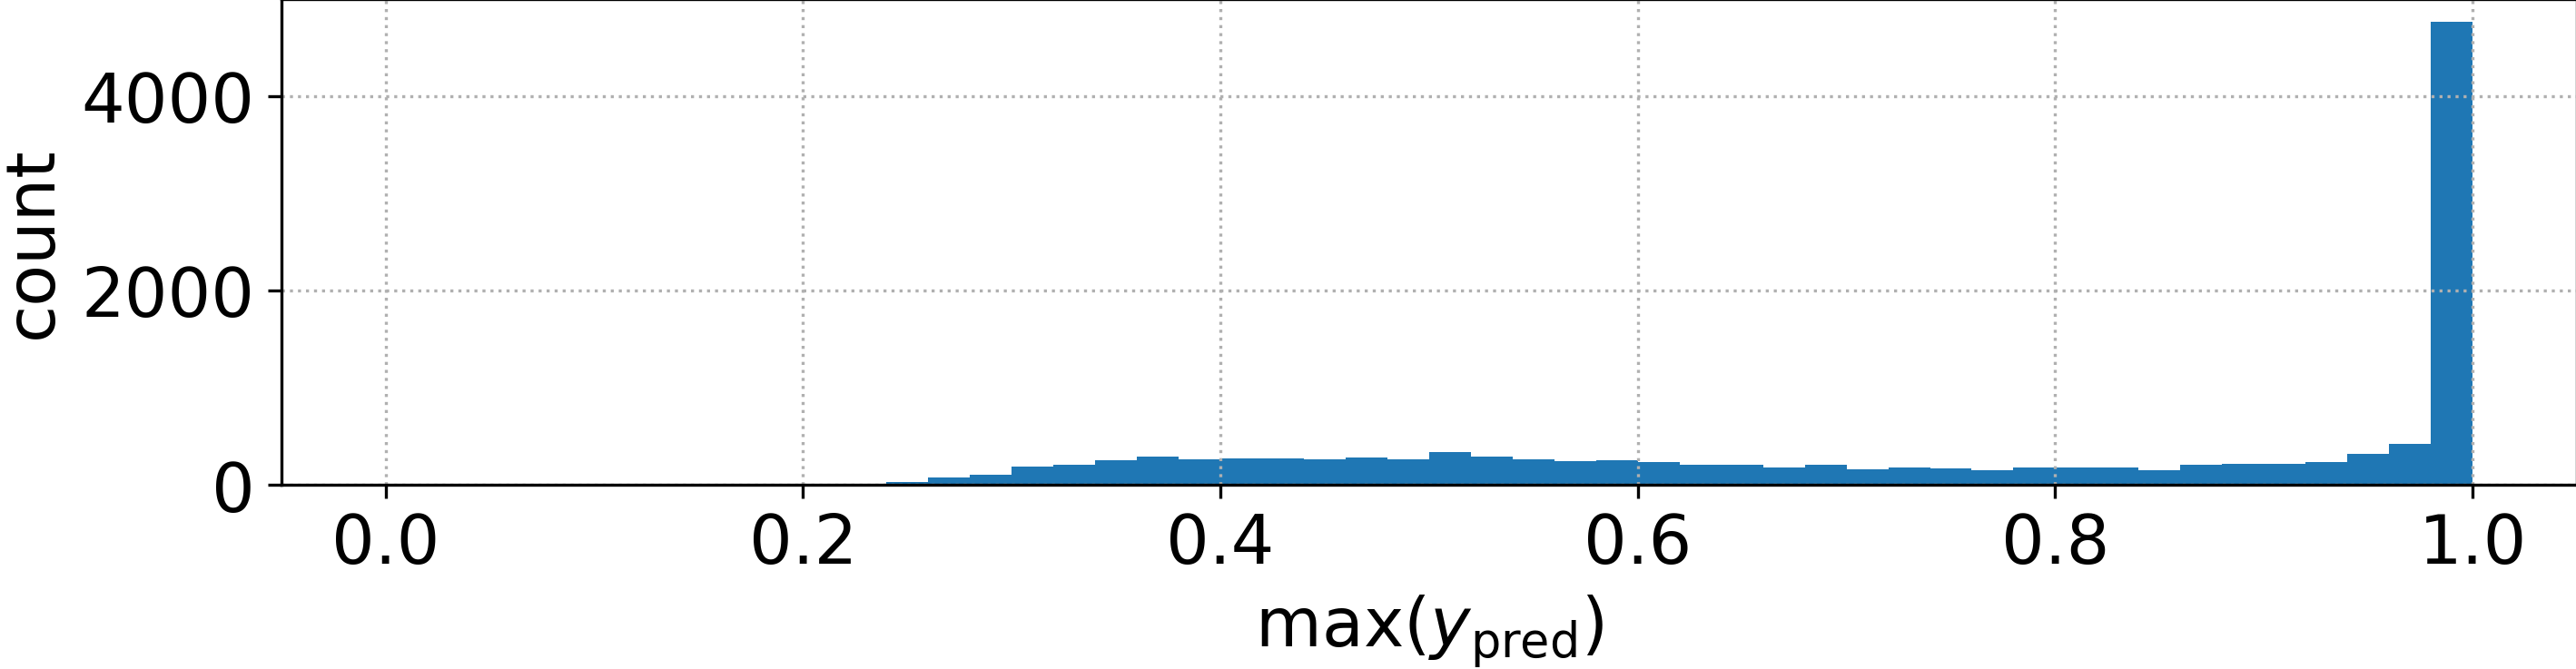
\includegraphics[width=0.8\textwidth]{figures/v2_real/vit_model_V2max_ypred_26.png}
    \caption[Spectral ViT V2 Confidence]{Max value of the output vector from the Spectral ViT V2.\label{fig:v2_max}}
\end{figure}

\begin{figure}[b!]
    \centering
    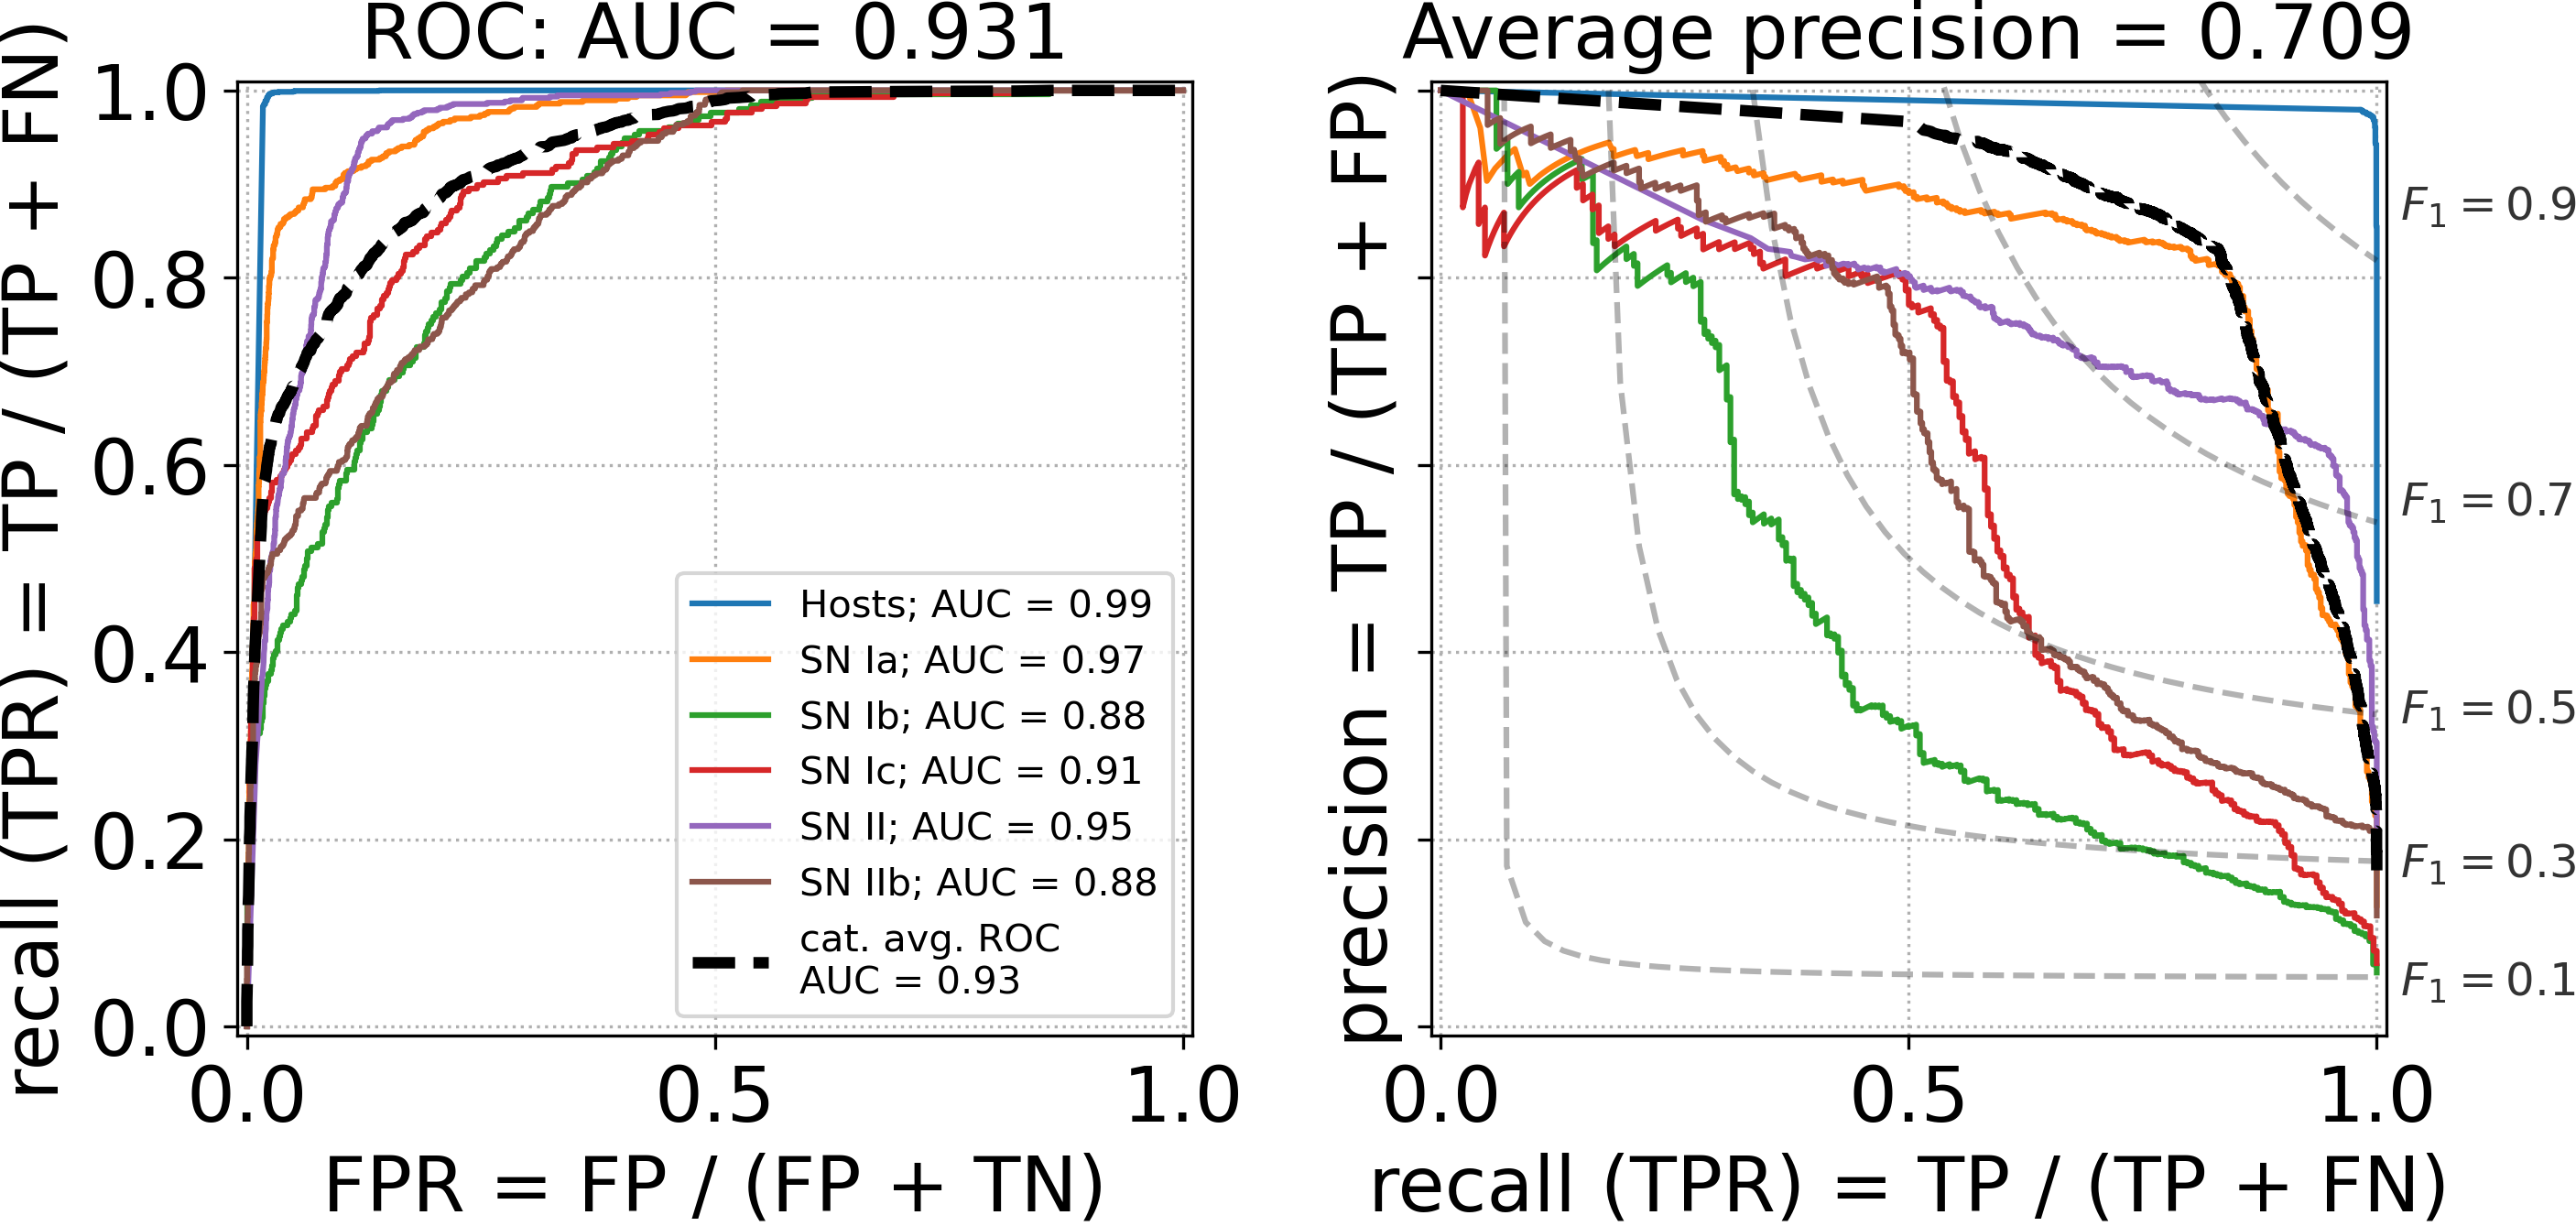
\includegraphics[height=4.3cm]{figures/v2_real/vit_model_V2roc99_e26.png}
    \quad
    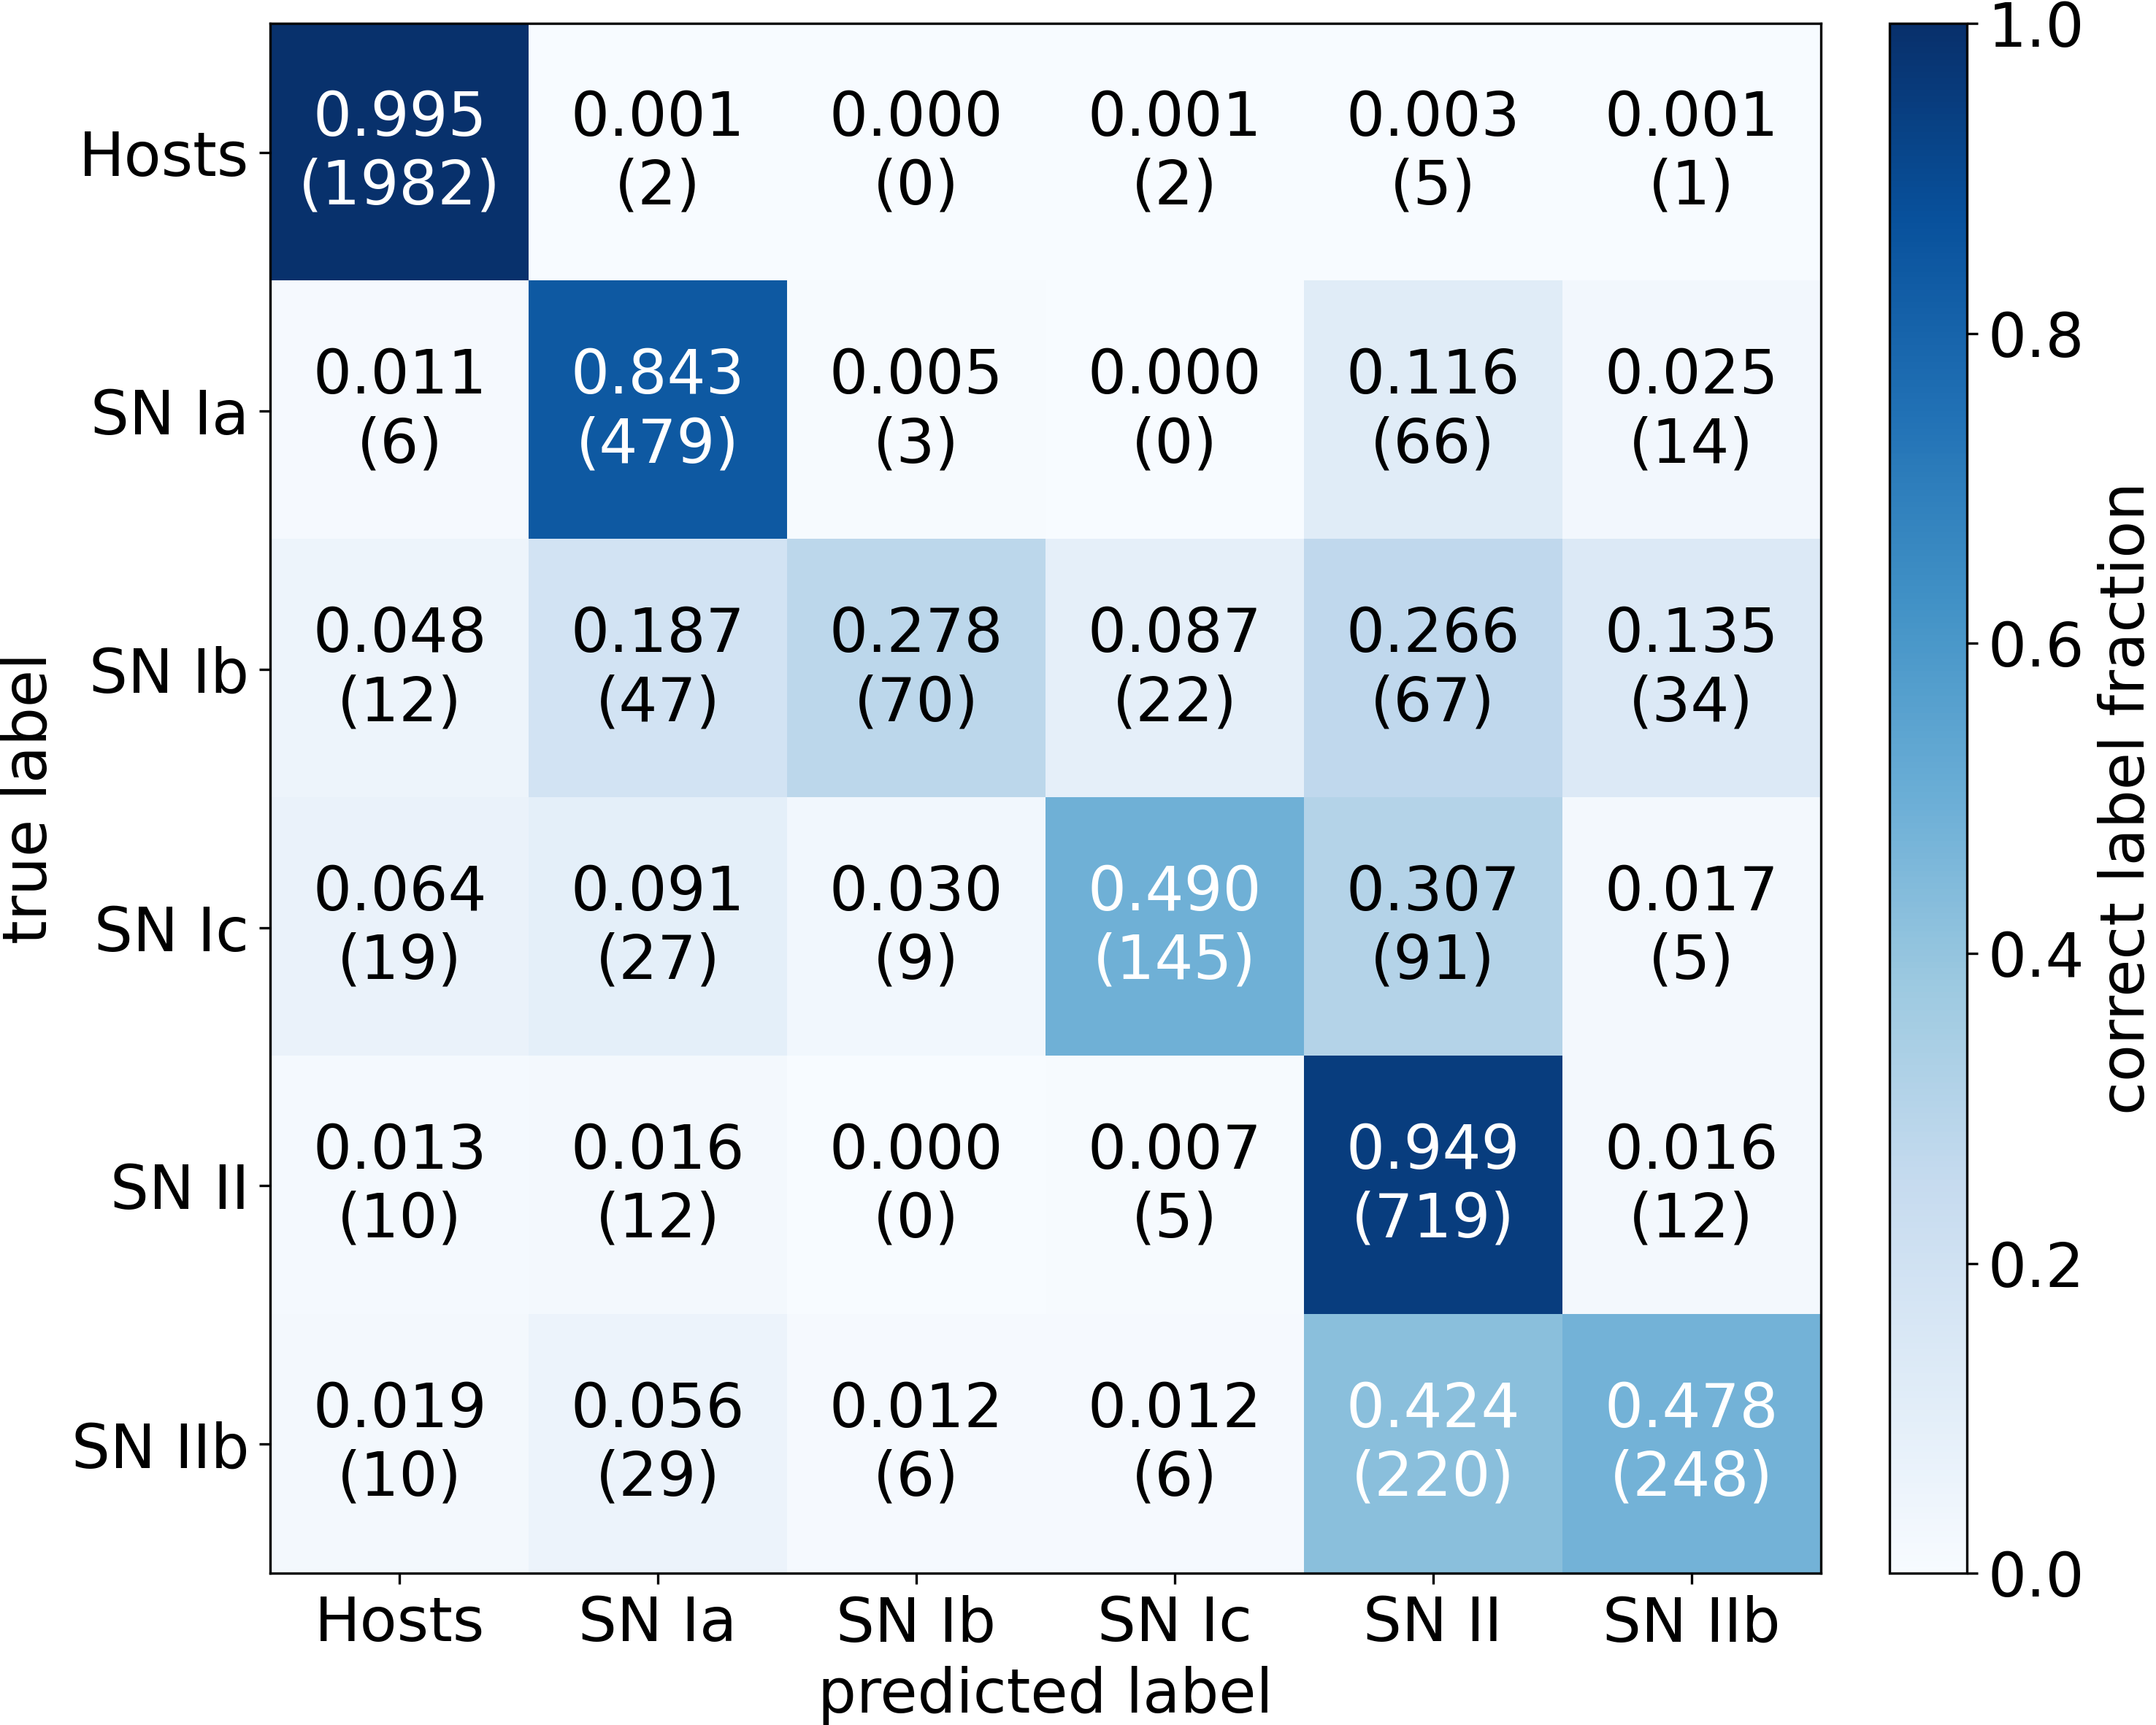
\includegraphics[height=4.3cm]{figures/v2_real/vit_model_V2cm99_e26.png}
    \caption[Spectral ViT V2 Diagnostics: 99\% Cut]{Spectral ViT V2 Diagnostics: ROC Curve (left) and Confusion Matrix (right) with a 99\% confidence
    cut\label{fig:v2_99_qual}}
\end{figure}

This, combined with the lower AUC score, indicates that the ViT V2 is not a suitable 
replacement for the ViT V1 for the purposes of SNe sub-type classification. However, the ViT V2
is still able to differentiate SNe and non-SNe spectra with high accuracy, so alternative uses 
can be derived from the existing classifier. 

\subsection{Alternative Applications of the V2 Classifier}

\subsubsection{Binary Classifier}

The most obvious use for a classifier capable of identifying the presence, or lack thereof, of a supernova 
with a high degree of accuracy is a binary classifier. To alter the predictions presented by the ViT 
for binary classification, the probabilities of all classes apart from 
non-SNe were summed. This resulted in a very high AUC score of 0.997, with a 
nearly perfect average precision of 98.7\% (Figure \ref{fig:v2_binary_qual}).
\begin{figure}[t!]
    \centering
    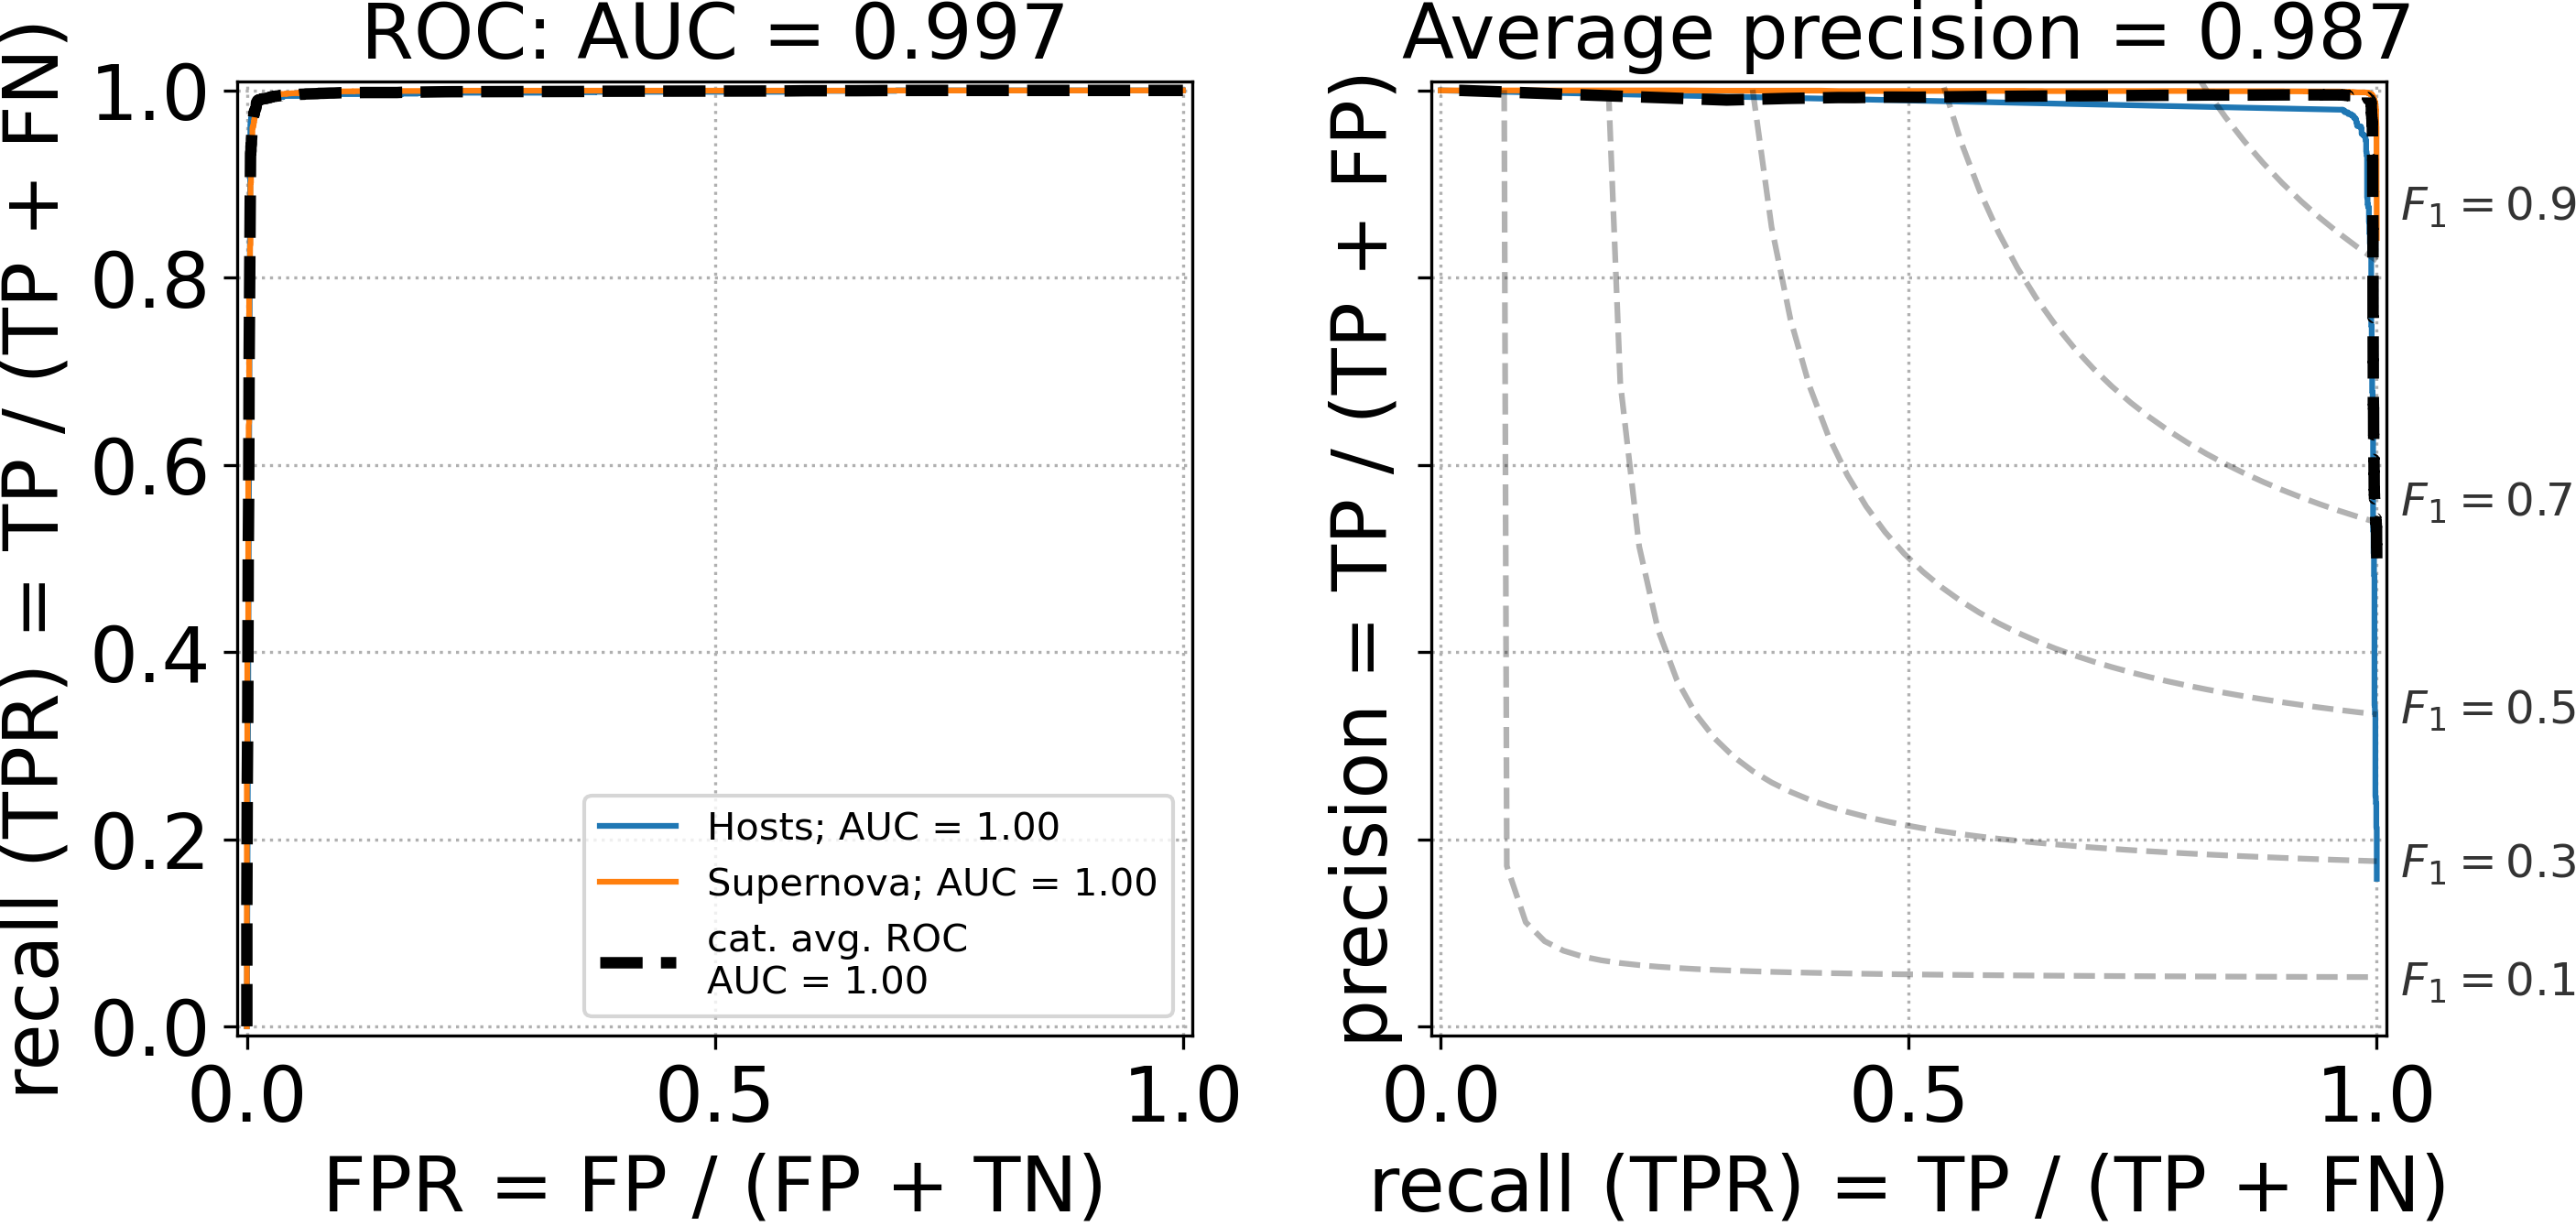
\includegraphics[height=4.2cm]{figures/v2_real/vit_model_V2rocfull_binary_e26.png}
    \quad
    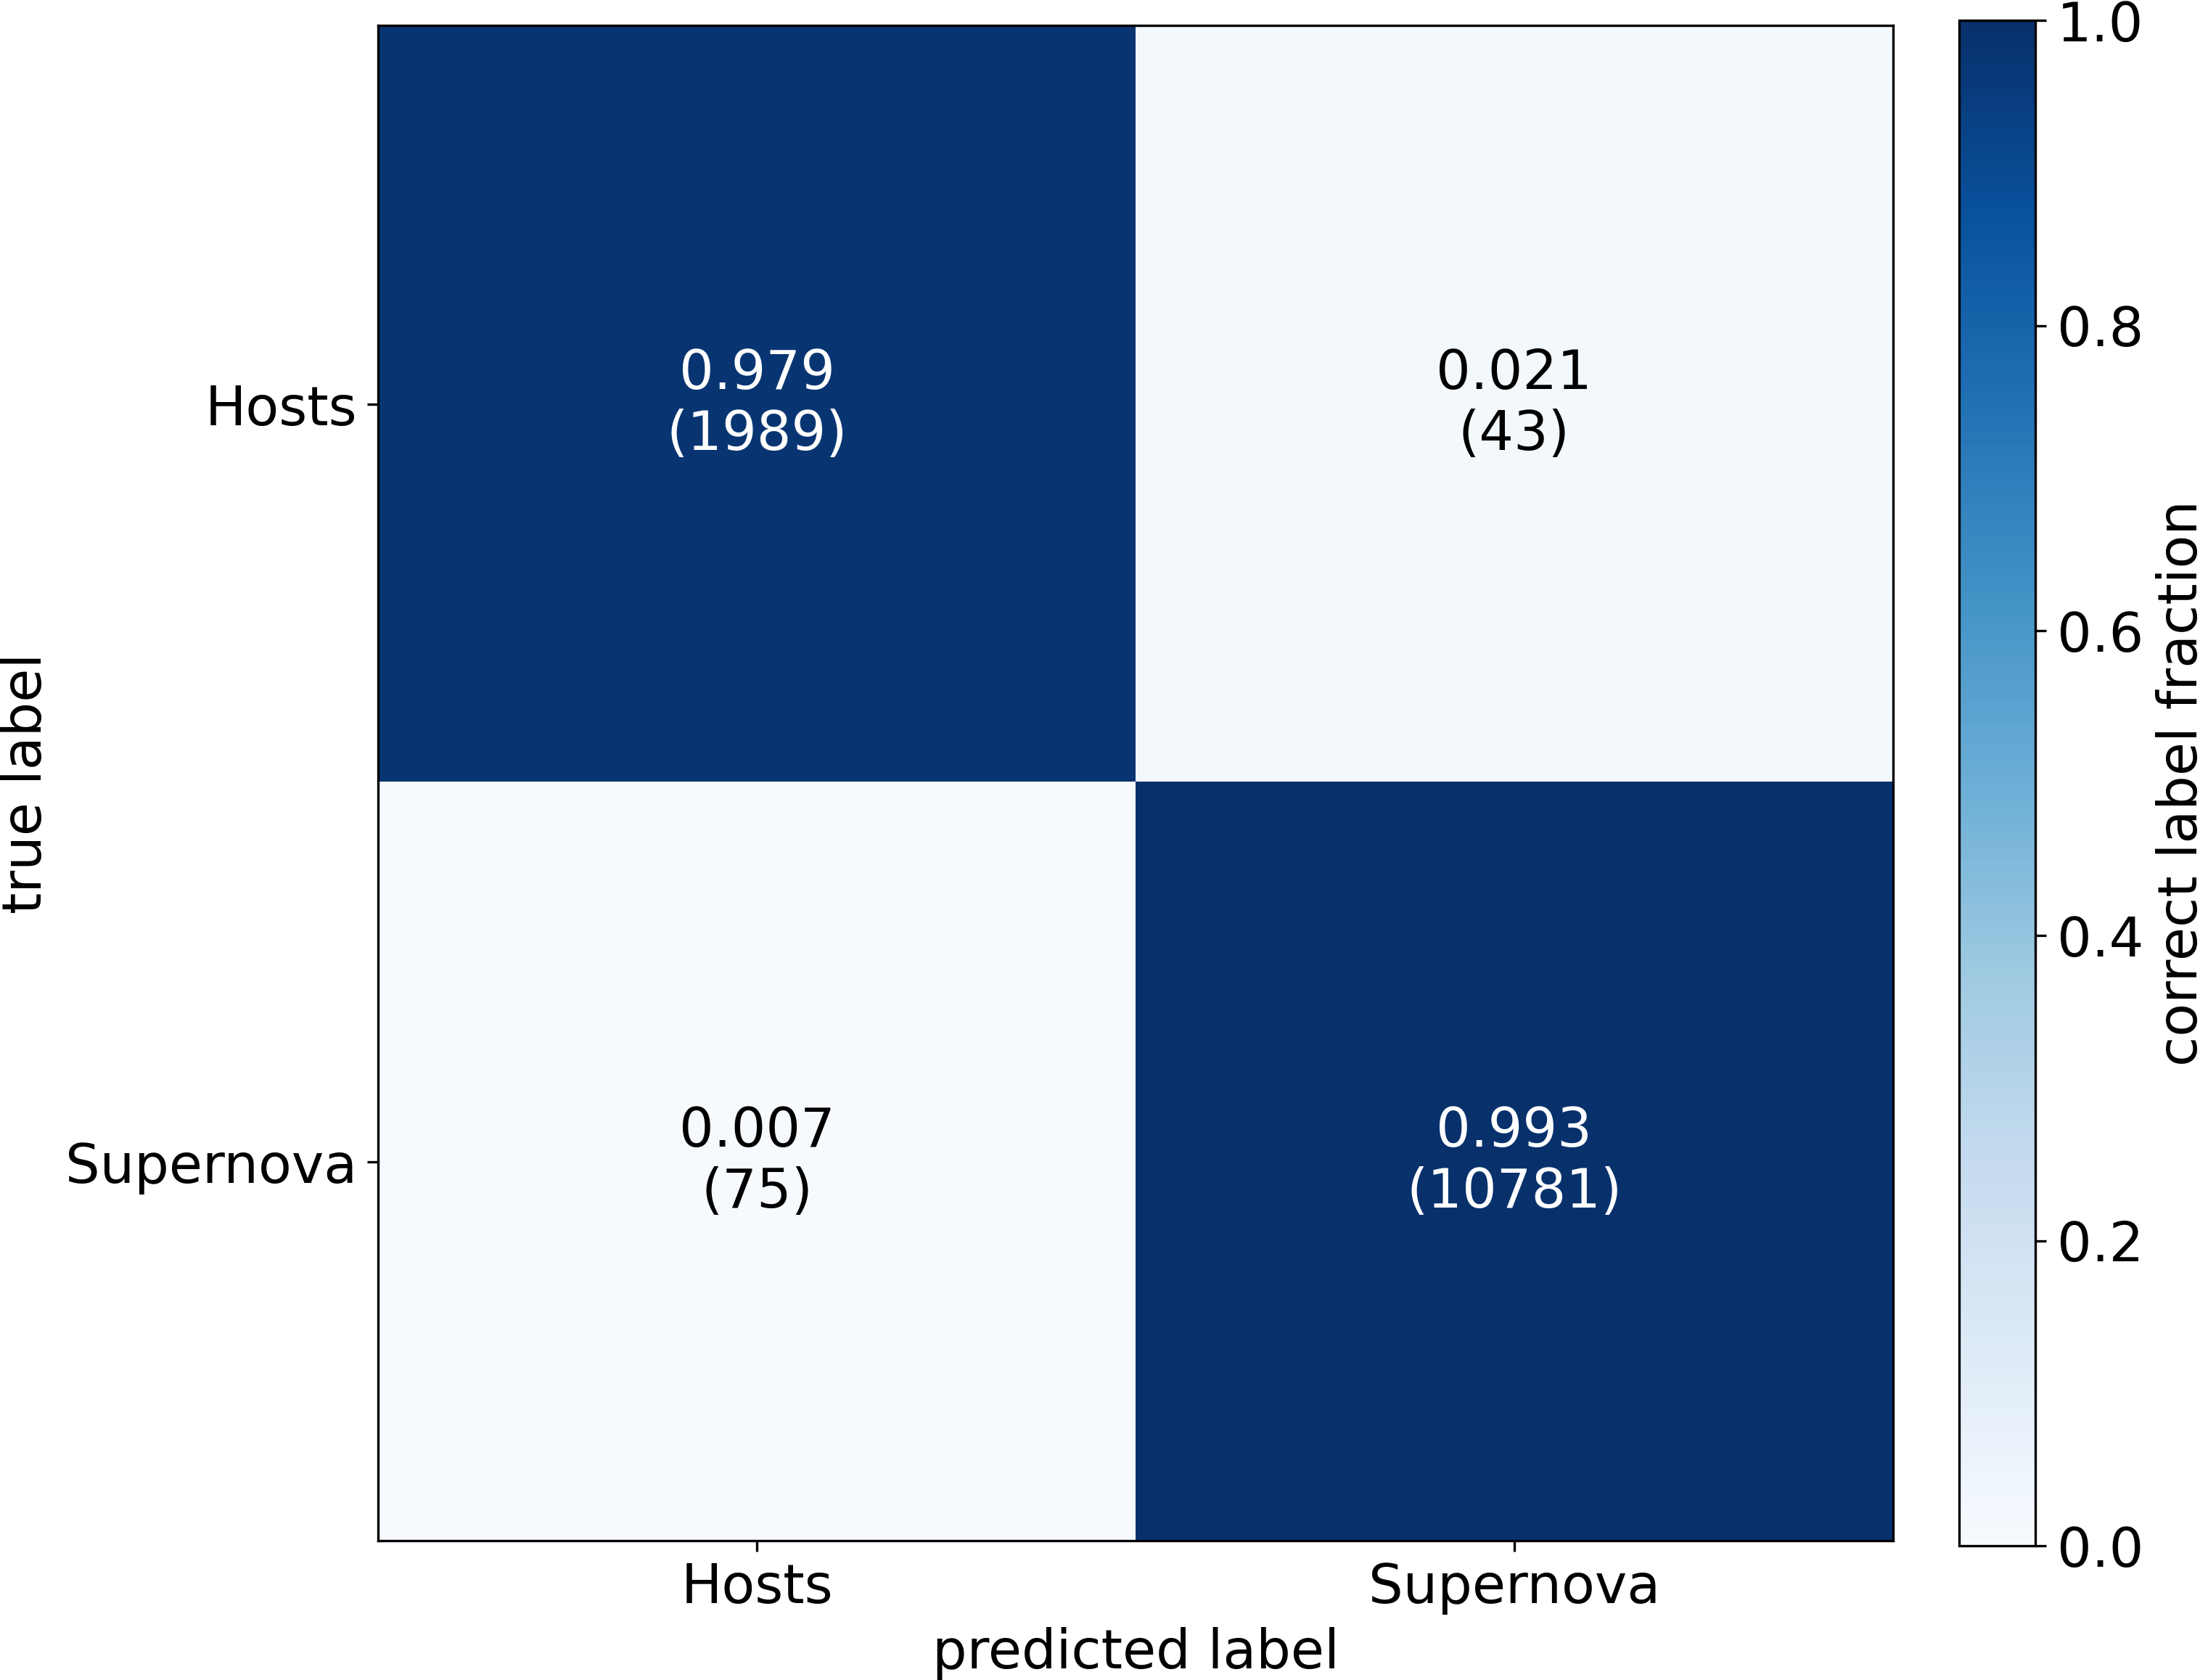
\includegraphics[height=4.2cm]{figures/v2_real/vit_model_V2cmfull_binary_e26.png}
    \caption[Spectral ViT V2 Binary Diagnostics]{Spectral ViT V2 Binary Diagnostics:
    ROC Curve (left) and Confusion Matrix (right)\label{fig:v2_binary_qual}}
\end{figure}
This, combined with the over 55\% of sample classifications having a prediction confidence of over 99.9999\%,
indicates the ViT V2's outstanding ability to act as a binary classifier for the presence of SNe.
% \begin{figure}[hb!]
%     \centering
%     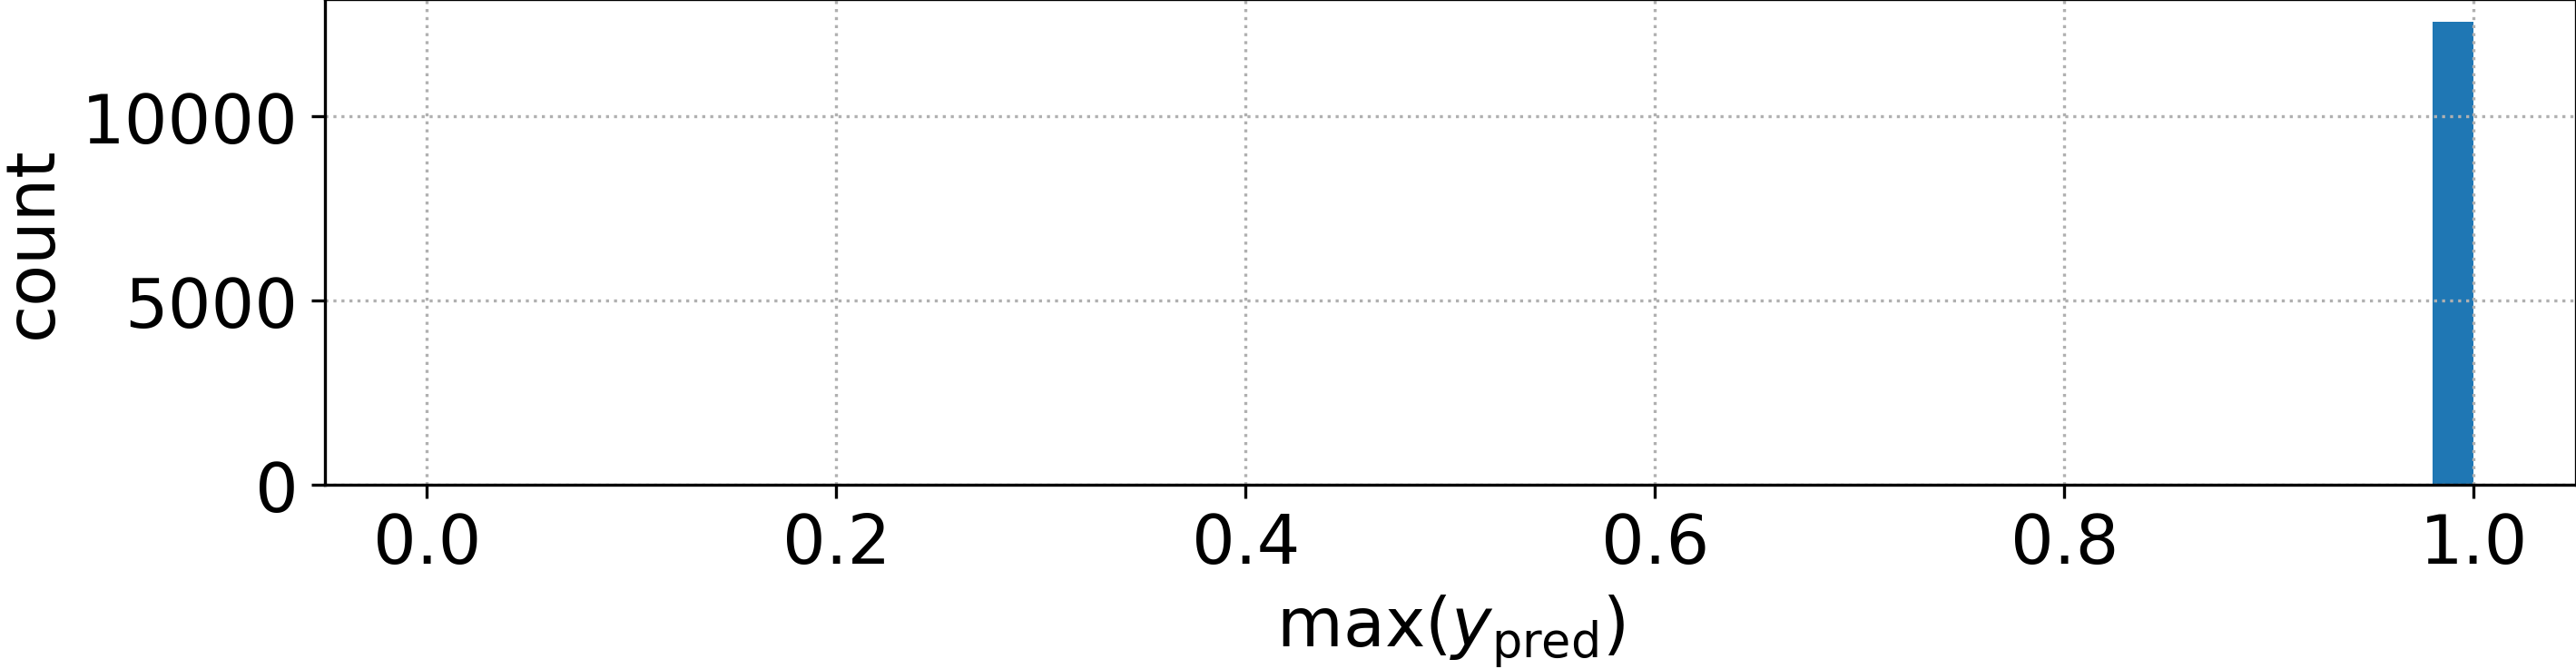
\includegraphics[width=0.8\textwidth]{figures/v2_real/vit_model_V2max_ypred_binary_26.png}
%     \caption[Spectral ViT V2 Confidence]{Max value of the output vector from the 
%     Spectral ViT V2 Binary Classification.\label{fig:v2_binary_max}}
% \end{figure}

\subsubsection{Progenitor and Type Classification}
\begin{figure}[htb!]
    \centering
    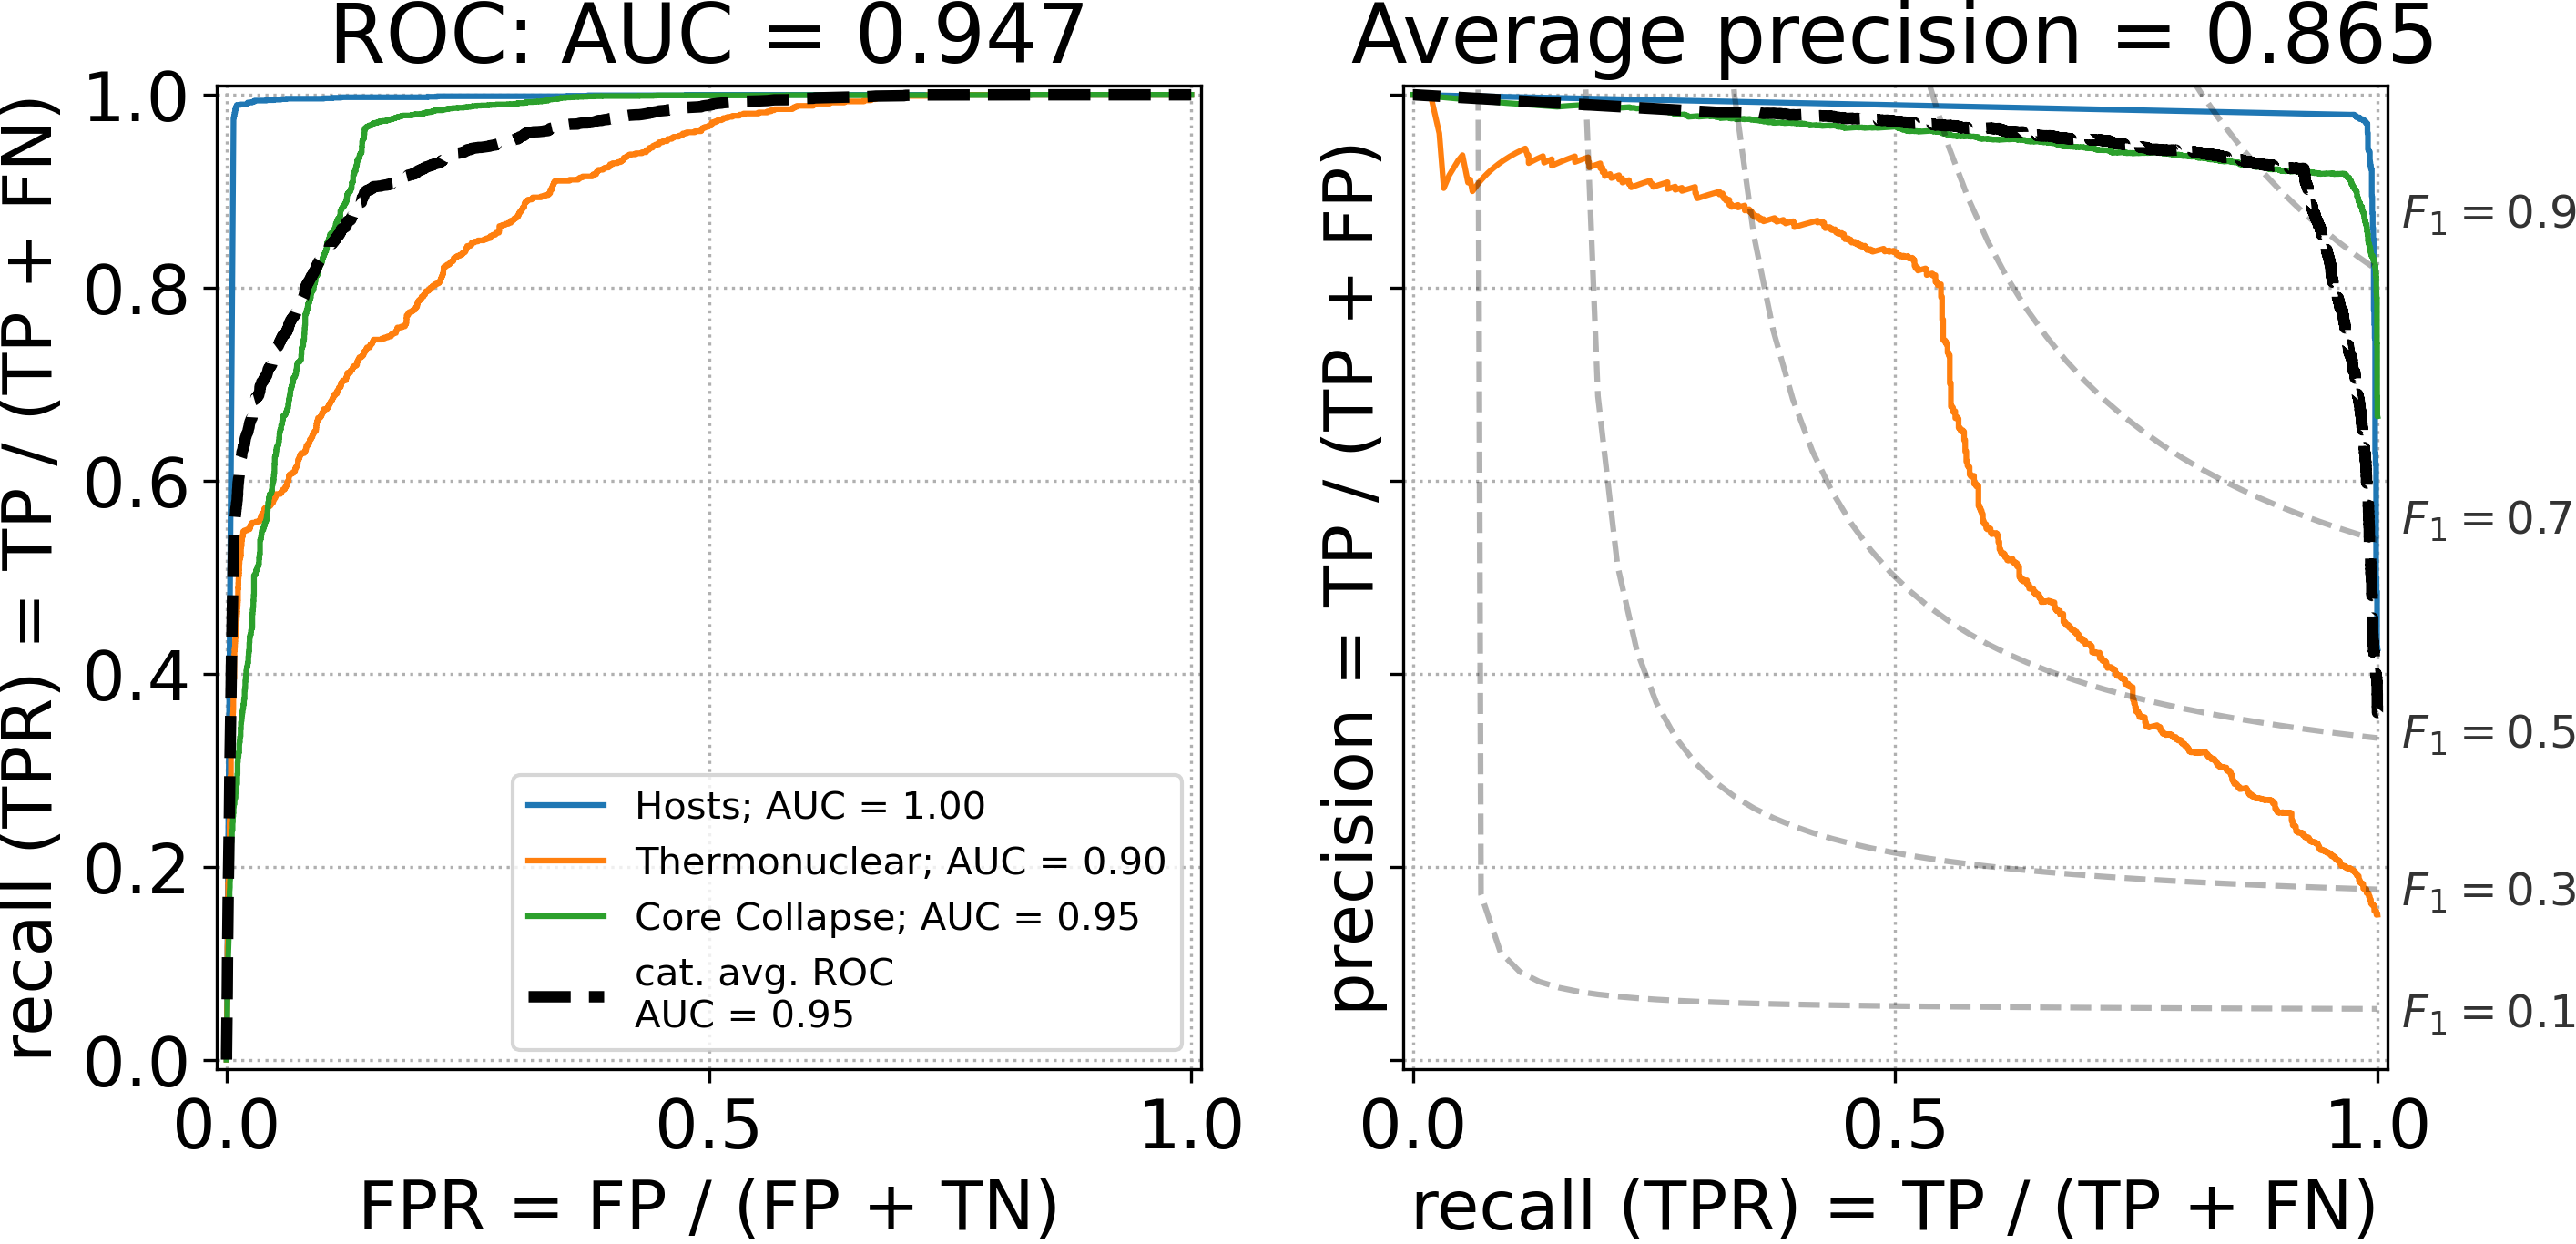
\includegraphics[height=4.1cm]{figures/v2_applications/vit_model_V2roc99_proj_e26.png}
    \quad
    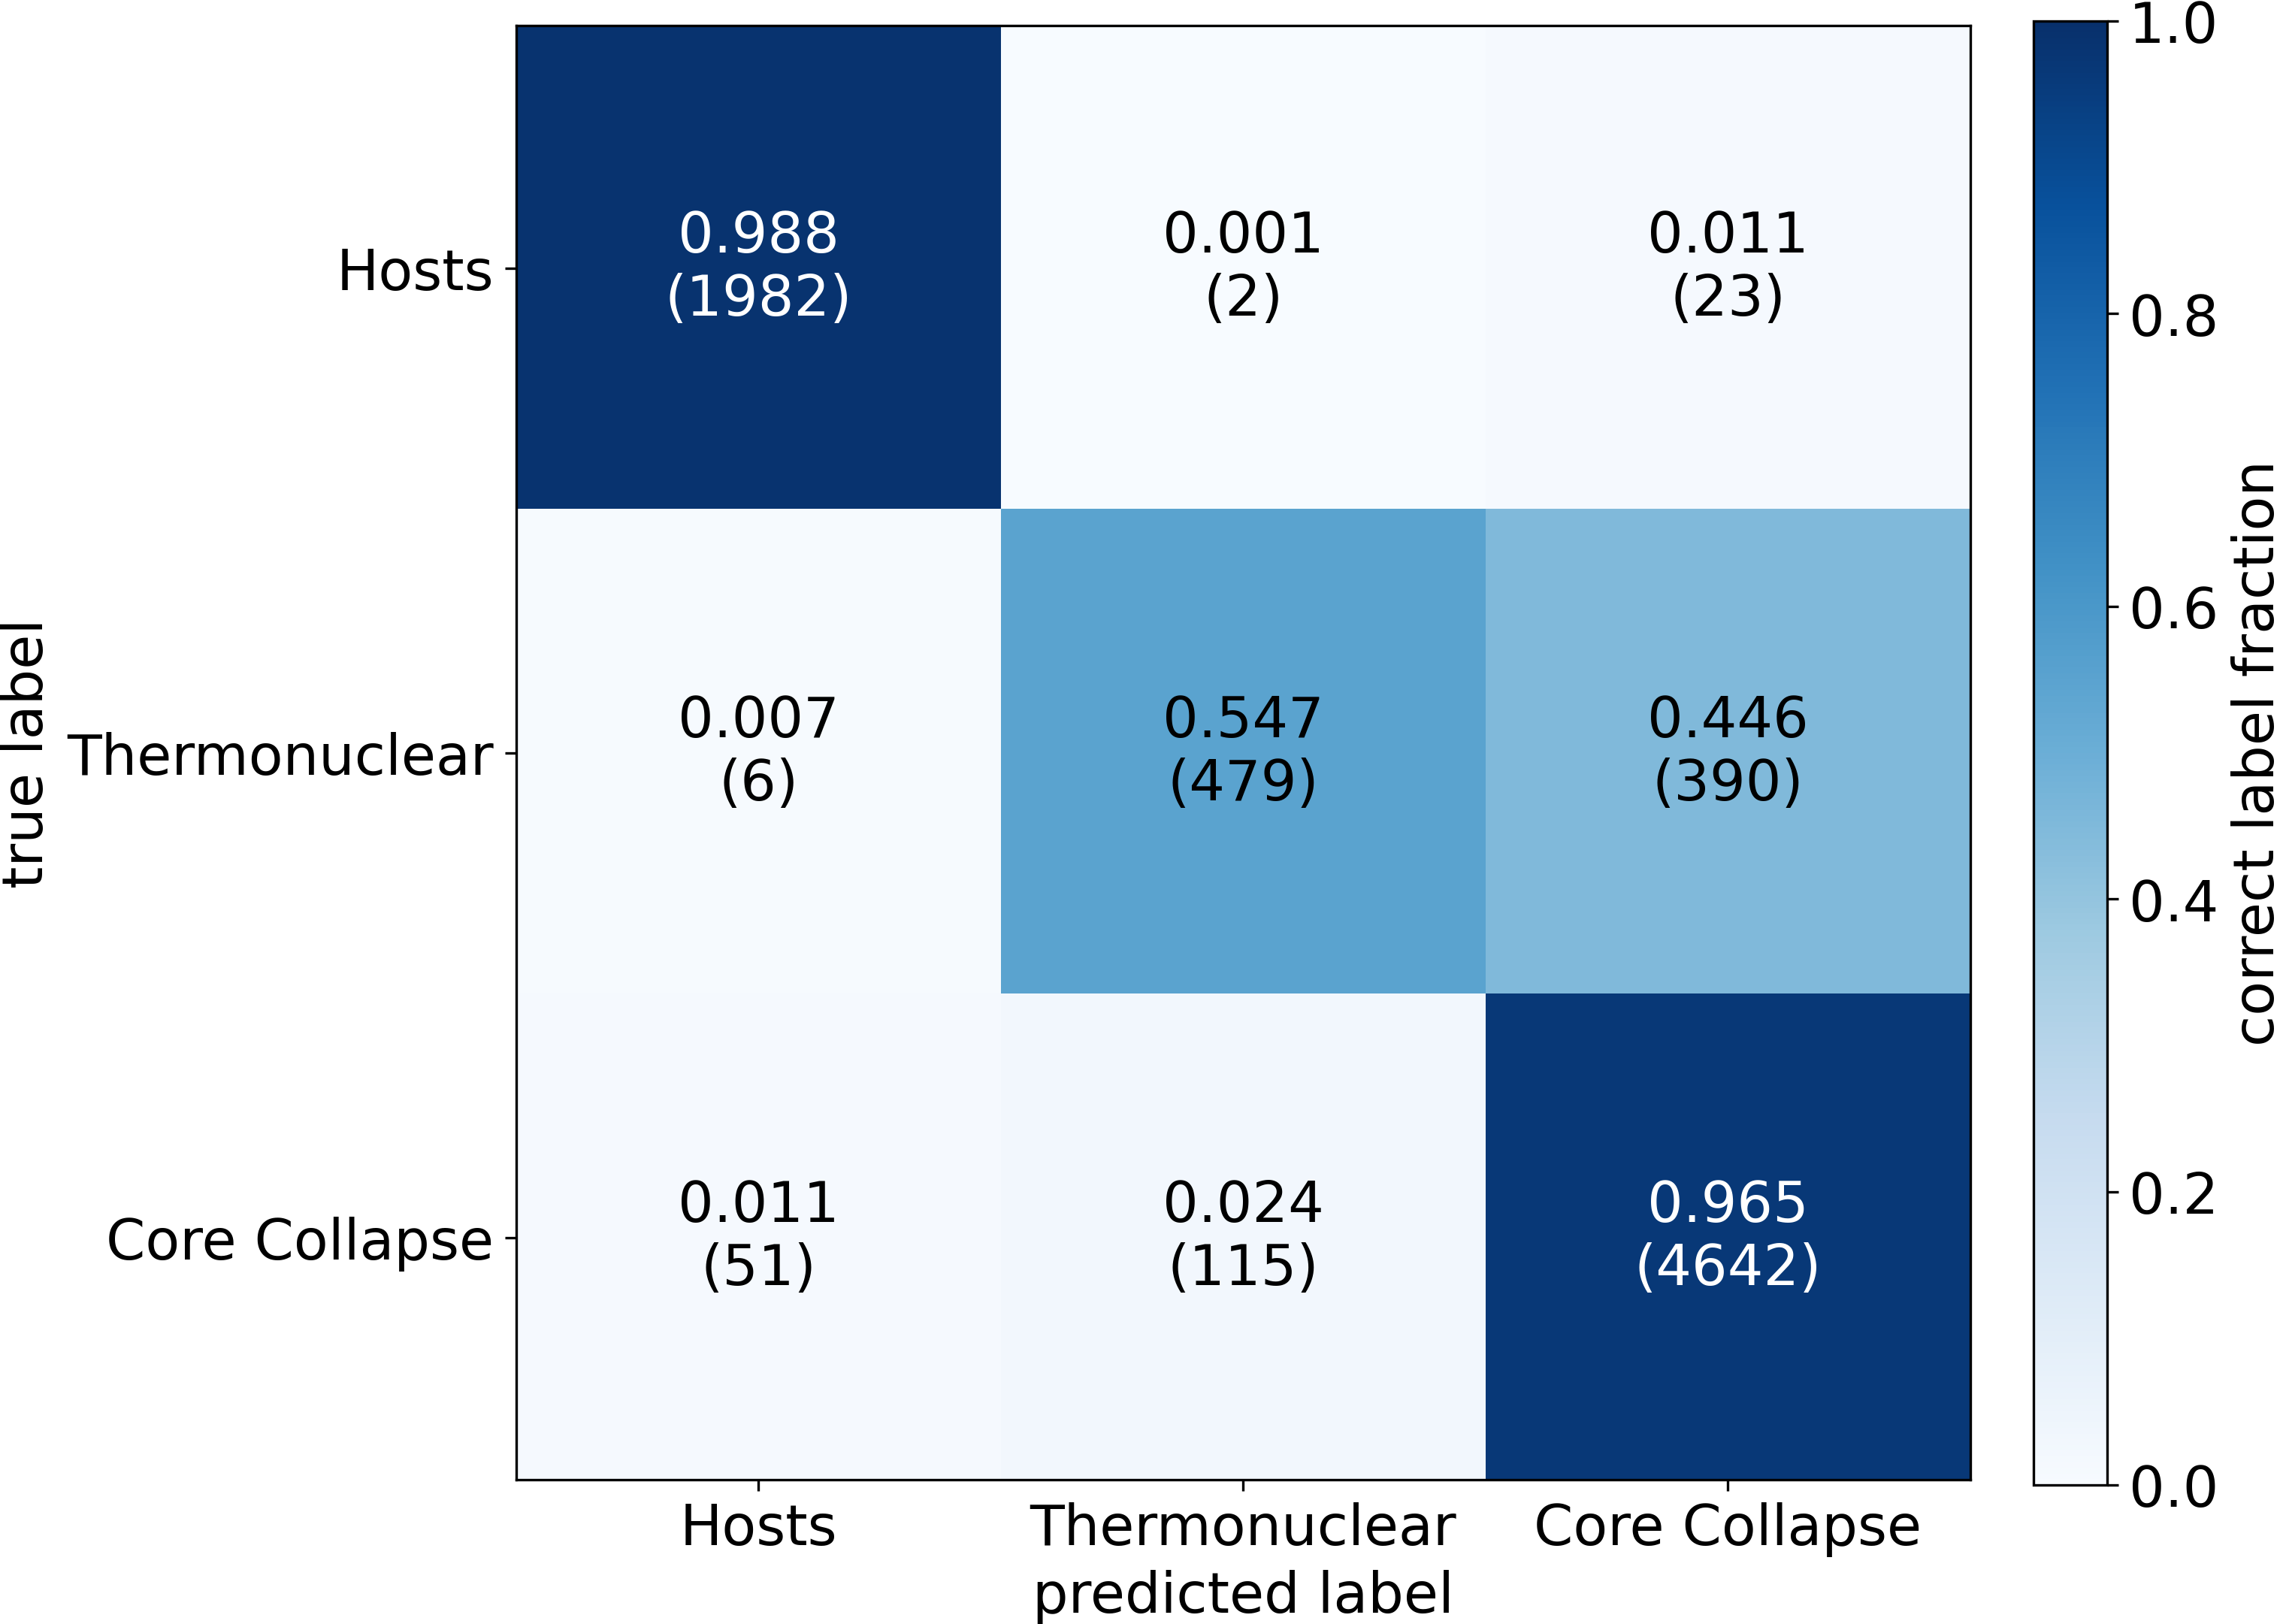
\includegraphics[height=4.1cm]{figures/v2_applications/vit_model_V2cm99_proj_e26.png}
    \caption[Spectral ViT V2 Progenitor Classifier Diagnostics]{Spectral ViT V2 
    Progenitor Classifier Diagnostics: ROC Curve (left) and Confusion Matrix (right) with a 99\% confidence
    cut\label{fig:v2_99_proj_qual}}
\end{figure}
Beyond binary classification, the Spectral ViT V2 shows the capability to differentiate between 
thermonuclear SNe (Type Ia) and core collapse SNe (Types Ib,c, and Type II). With a 99\% confidence 
cut, the classifier is able to retain 60\% of the original sample, shown in Figure~\ref{fig:v2_99_proj_qual}. 
Despite the great success in differentiating the core collapse and non-SNe spectra, there is some discrepancy 
between the two SNe categories. This, however, still results in an average precision of 86.5\% which is slightly
below the Spectral ViT V1 classifier on all subtypes, while recovering much of the original sample. 
\begin{figure}[hb!]
    \centering
    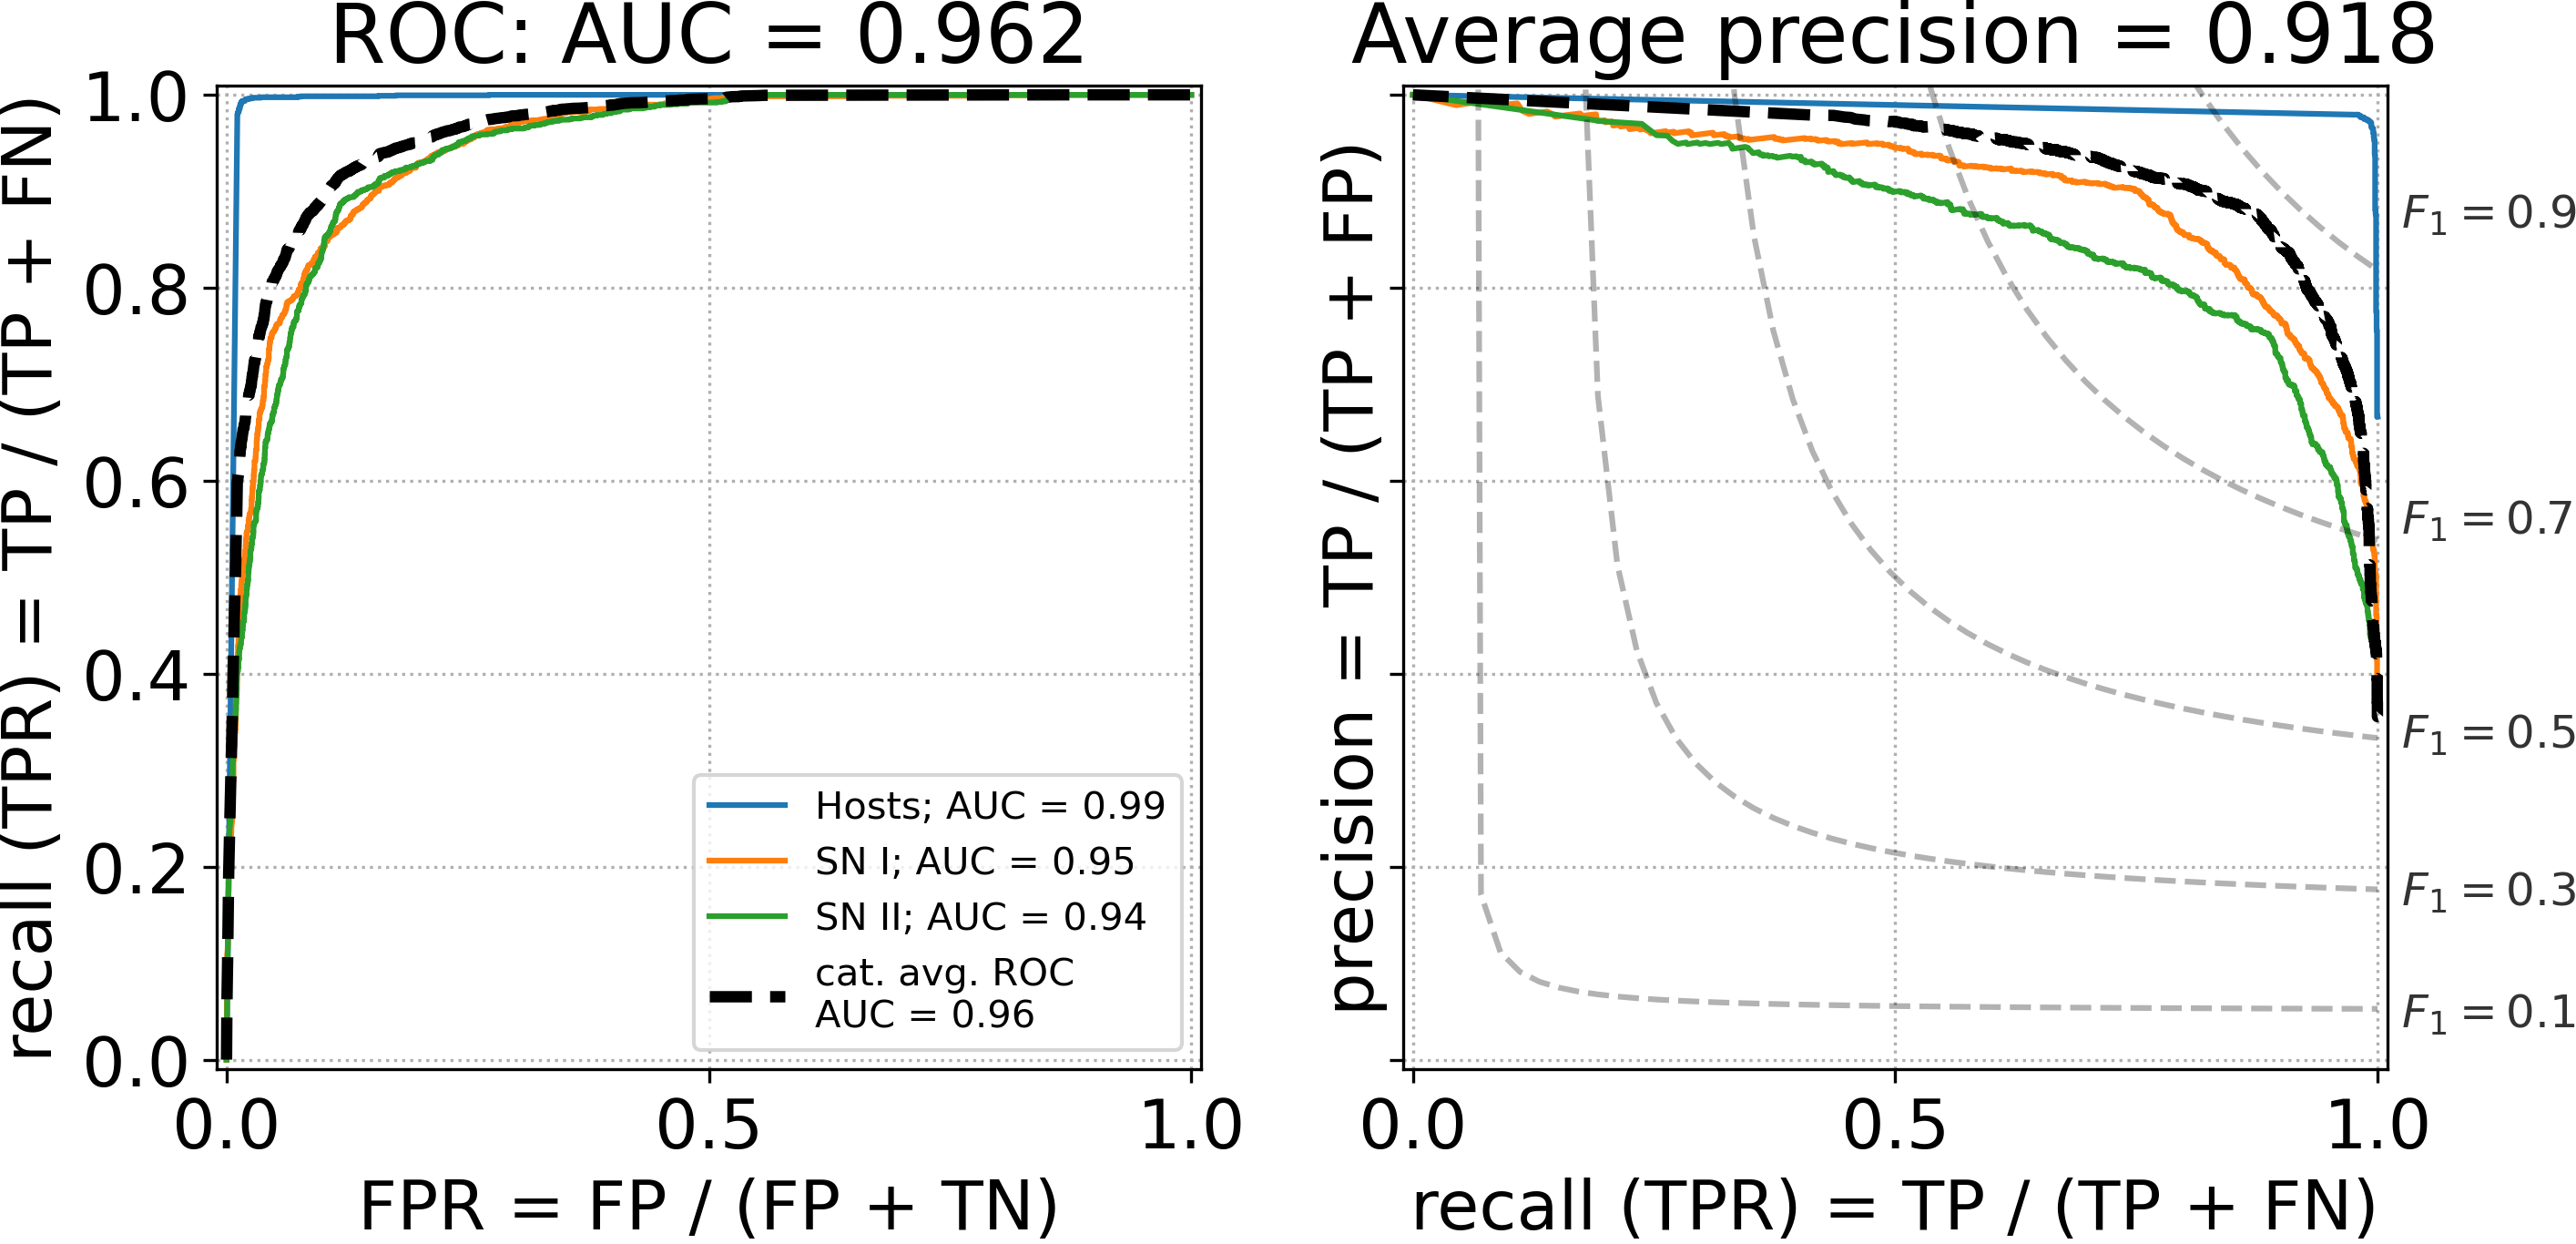
\includegraphics[height=4.1cm]{figures/v2_applications/vit_model_V2roc99_type_e26.png}
    \quad
    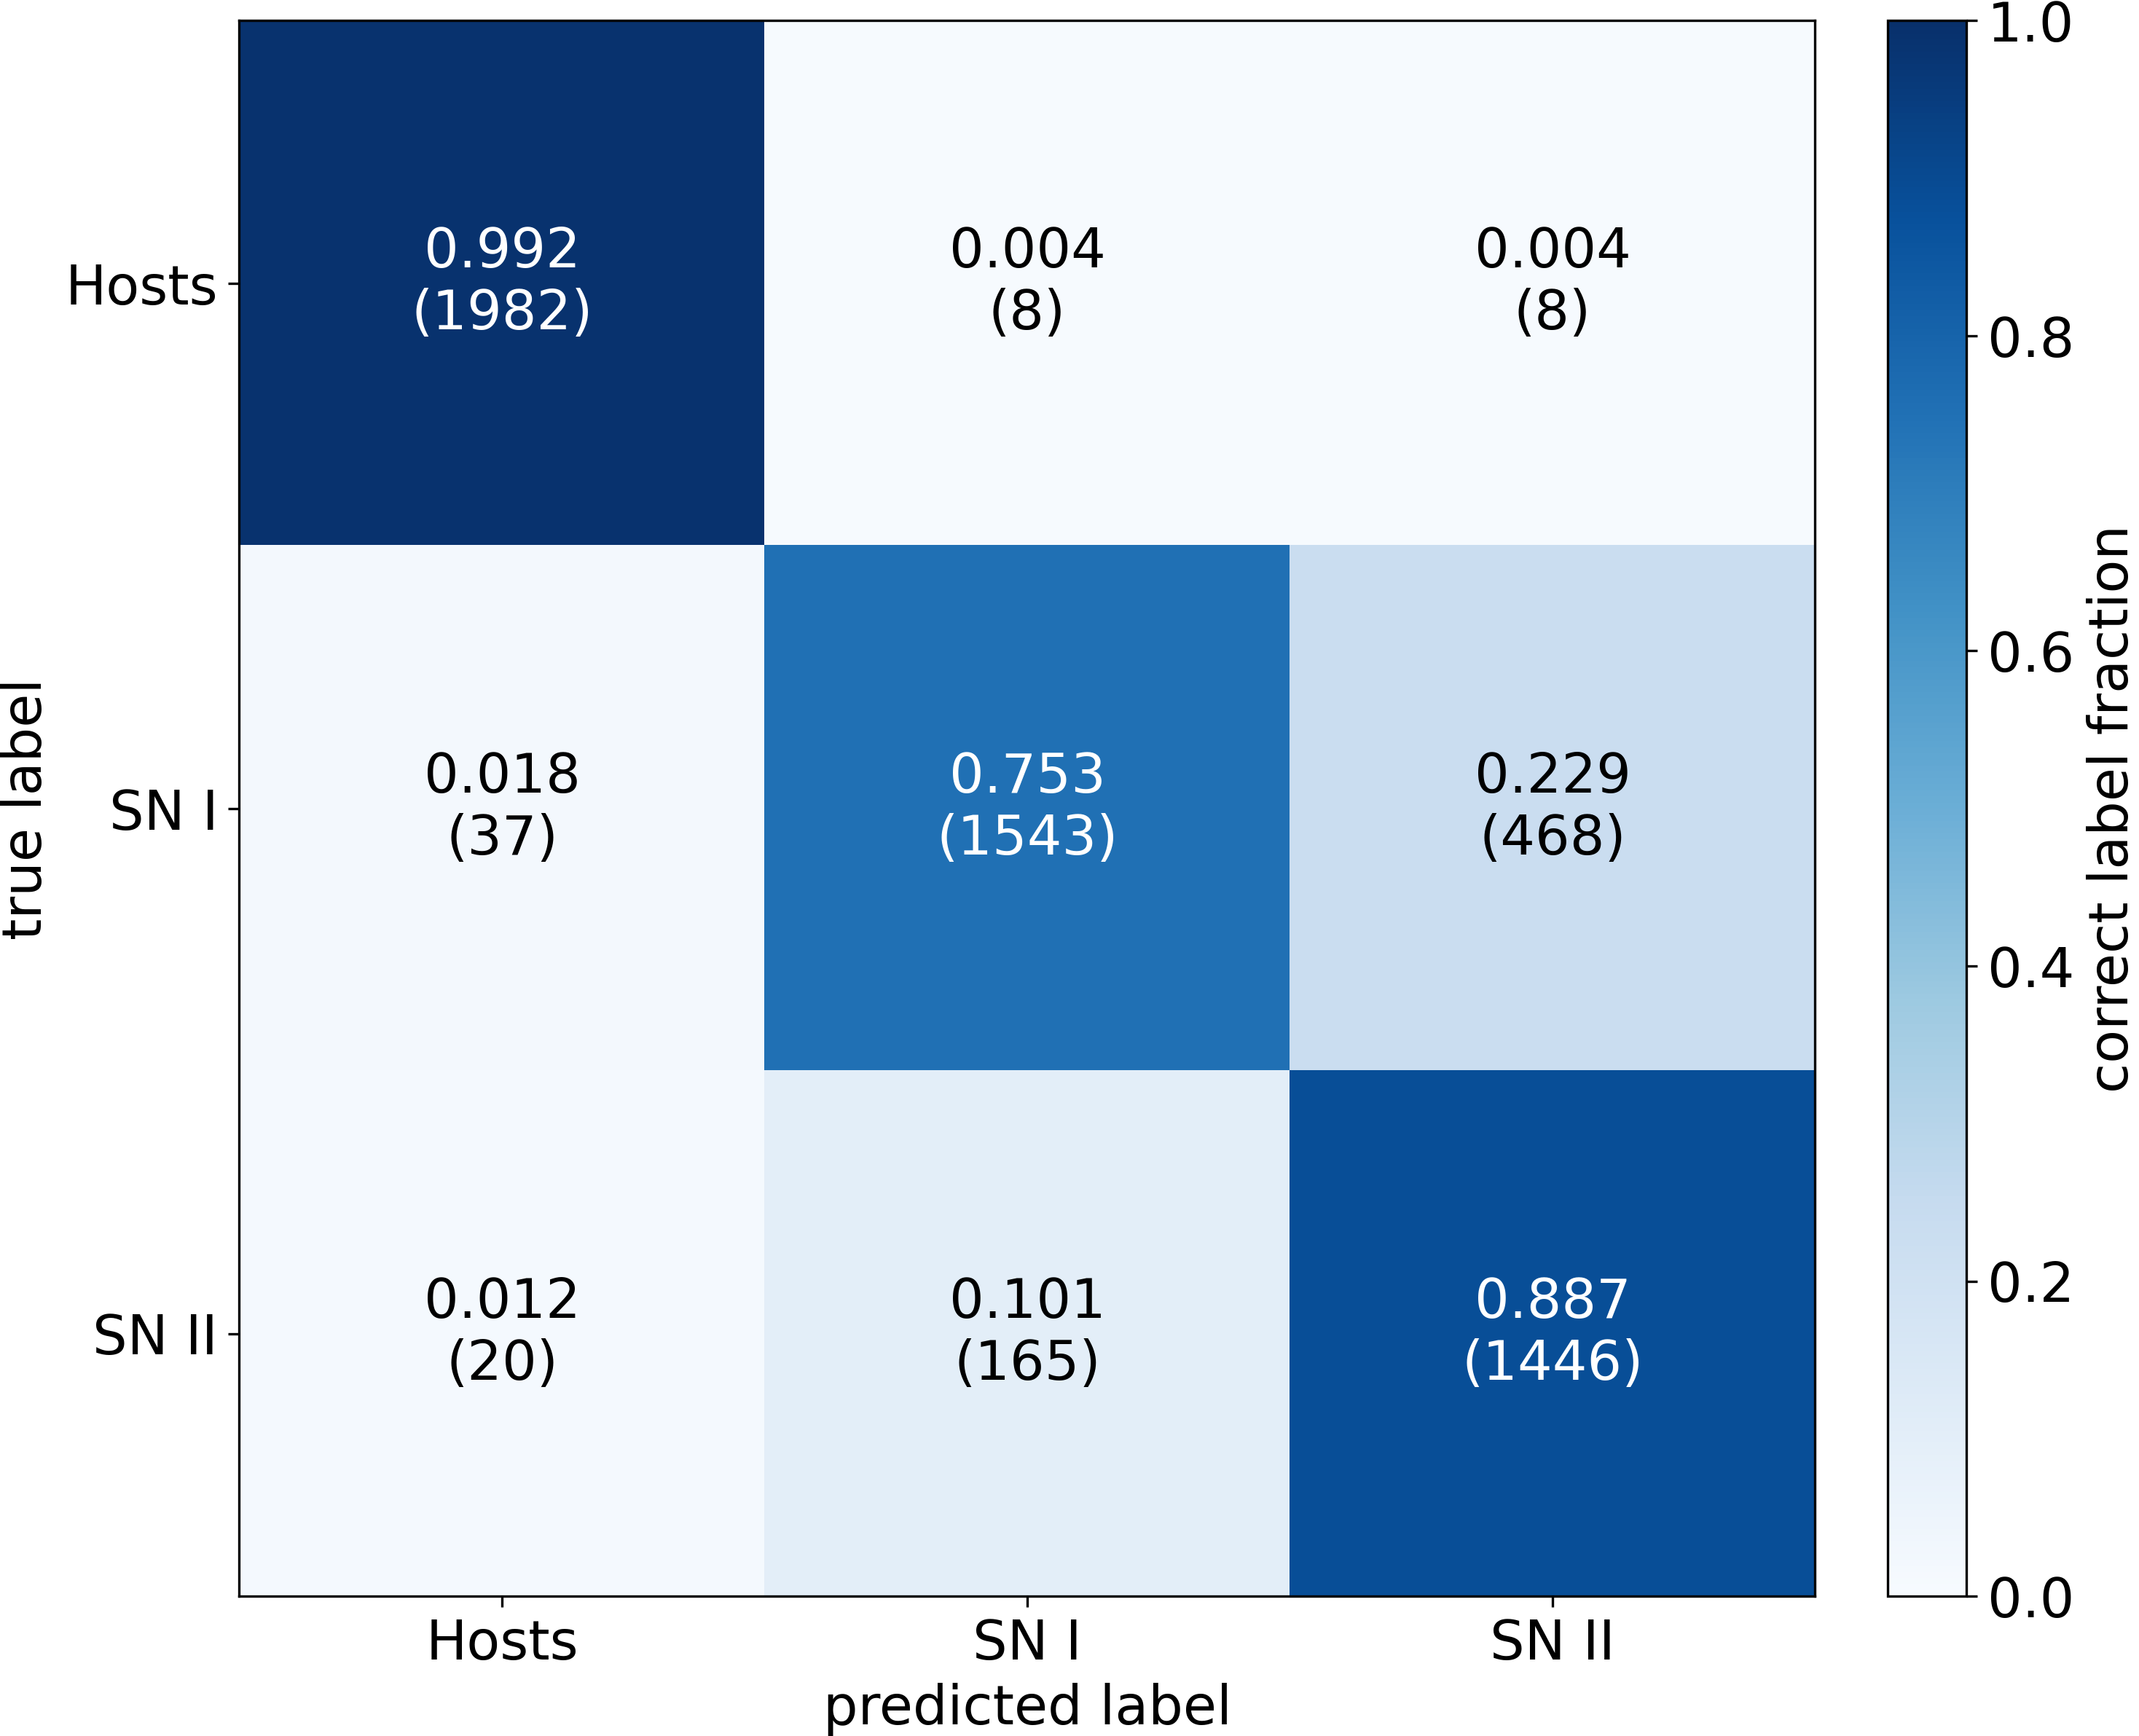
\includegraphics[height=4.1cm]{figures/v2_applications/vit_model_V2cm99_type_e26.png}
    \caption[Spectral ViT V2 Type Classifier Diagnostics]{Spectral ViT V2 
    Type Classifier Diagnostics: ROC Curve (left) and Confusion Matrix (right) with a 99\% confidence
    cut\label{fig:v2_99_type_qual}}
\end{figure}
Another classification scheme using three final classes would be to seperate the sample into the 2 main 
classifications: Type I vs Type II. Figure~\ref{fig:v2_99_type_qual} shows the 99\% cut on this classifications, 
yielding 44\% of the original sample classified at an average precision of 91.8\%. Therefore, the Spectral ViT V2
has many classification applications past just a binary classifier, regardless of its inability to produce precise 
classification of SNe subtypes.



% \begin{figure}[h]
%     \centering
%     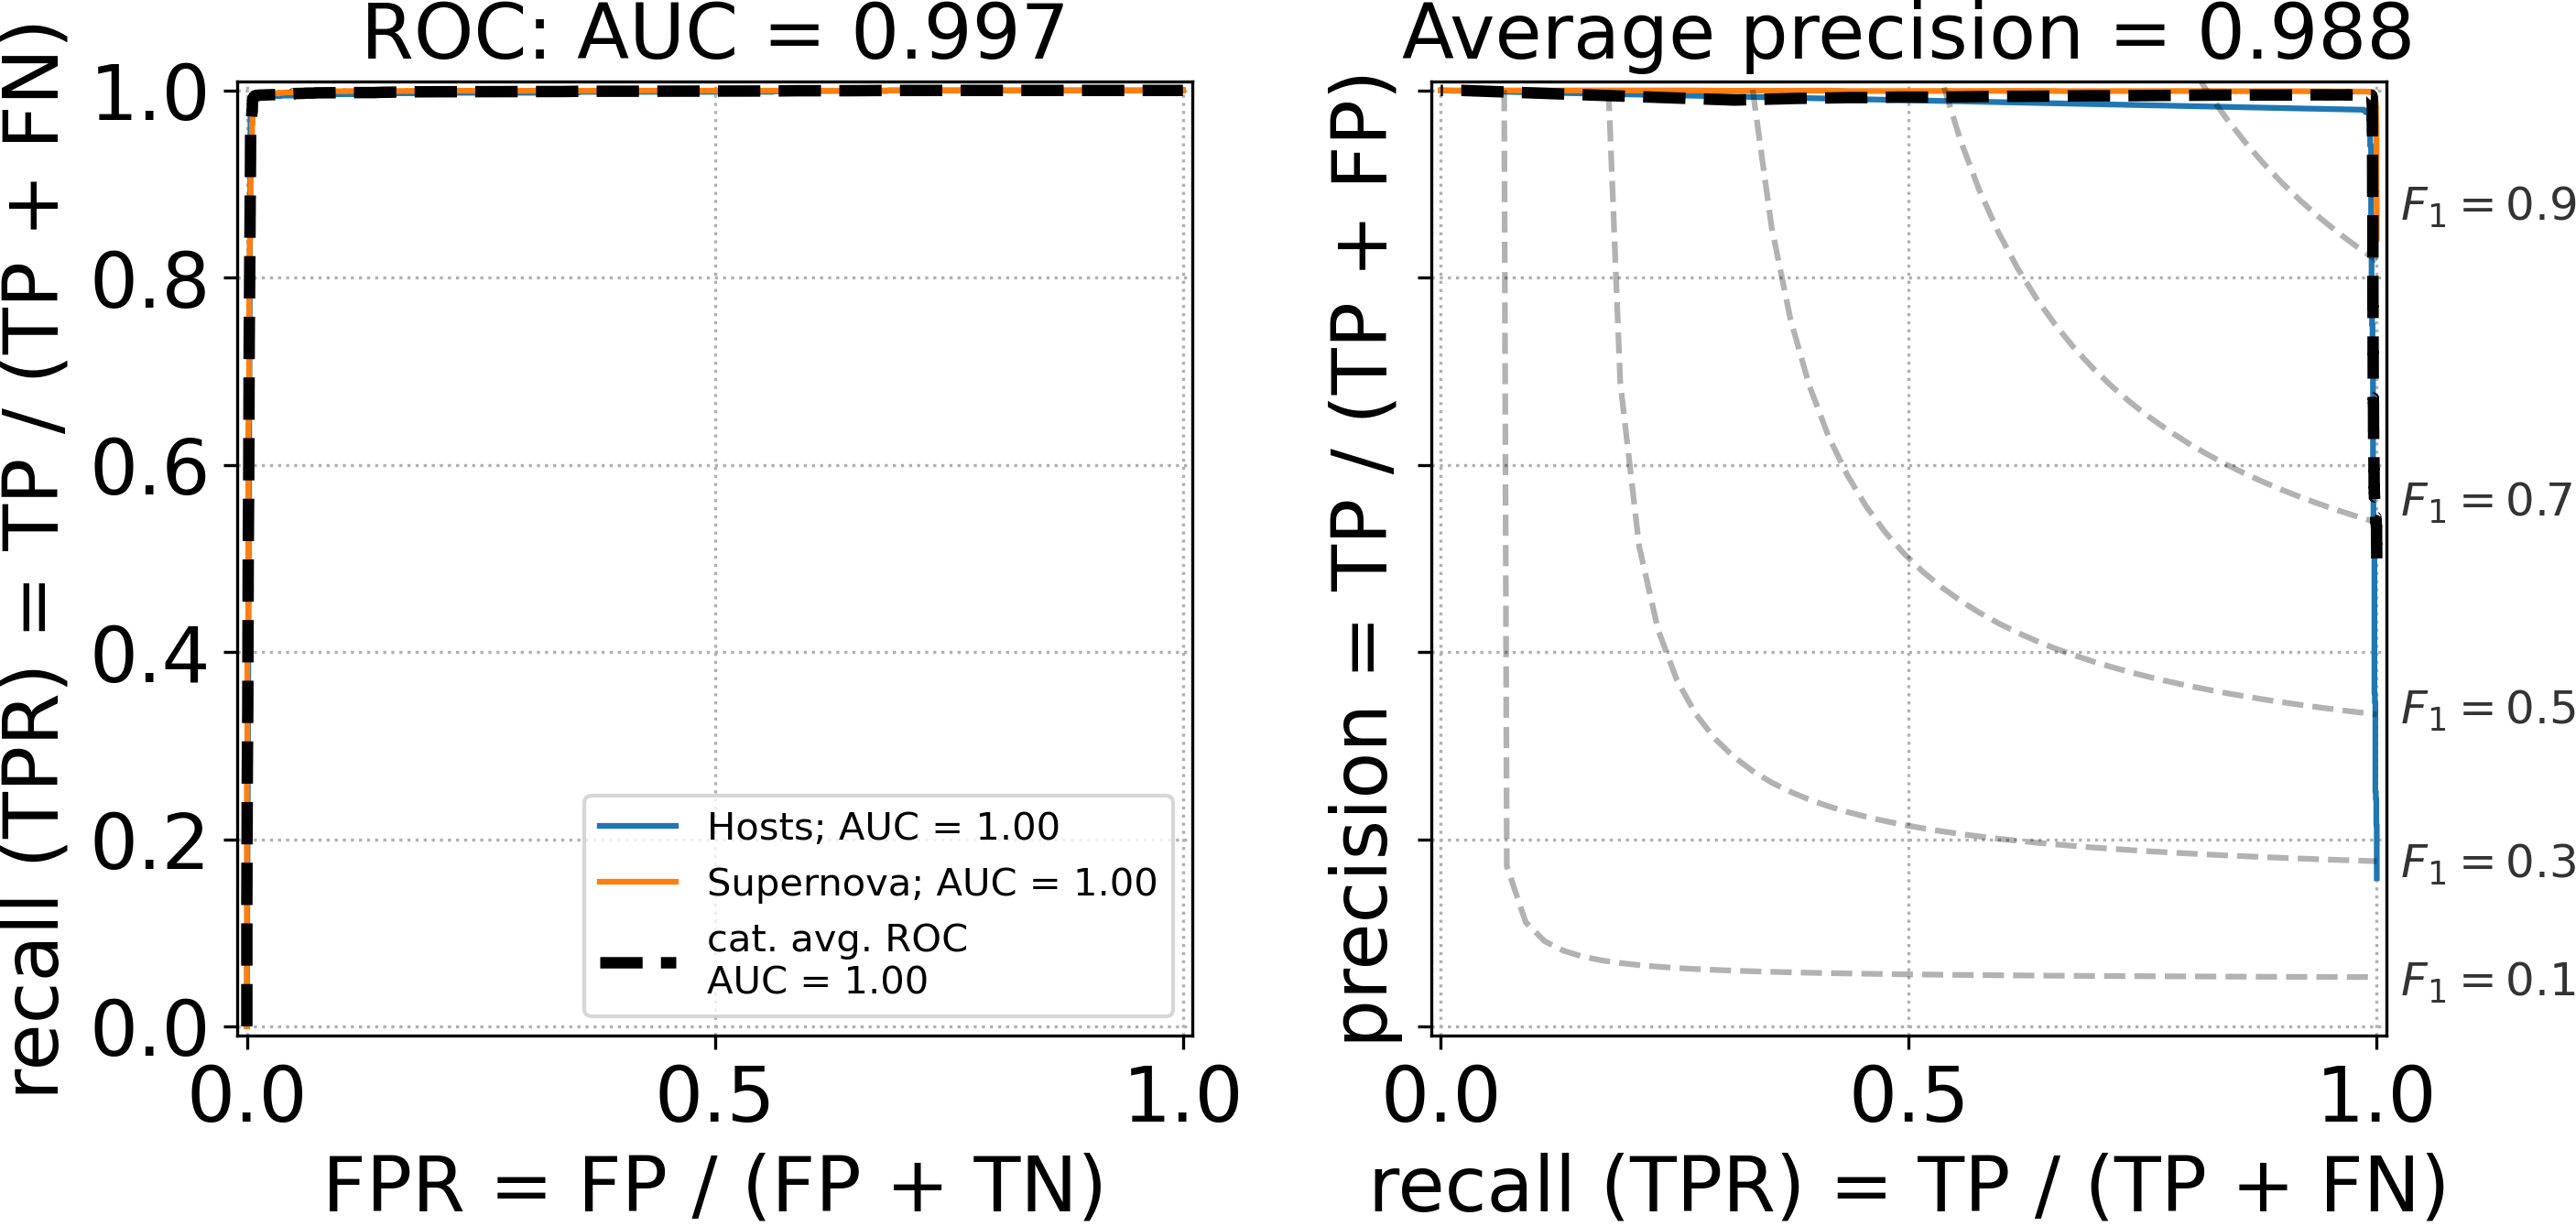
\includegraphics[height=4.2cm]{figures/v2_real/vit_model_V2roc9999_binary_e26.png}
%     \quad
%     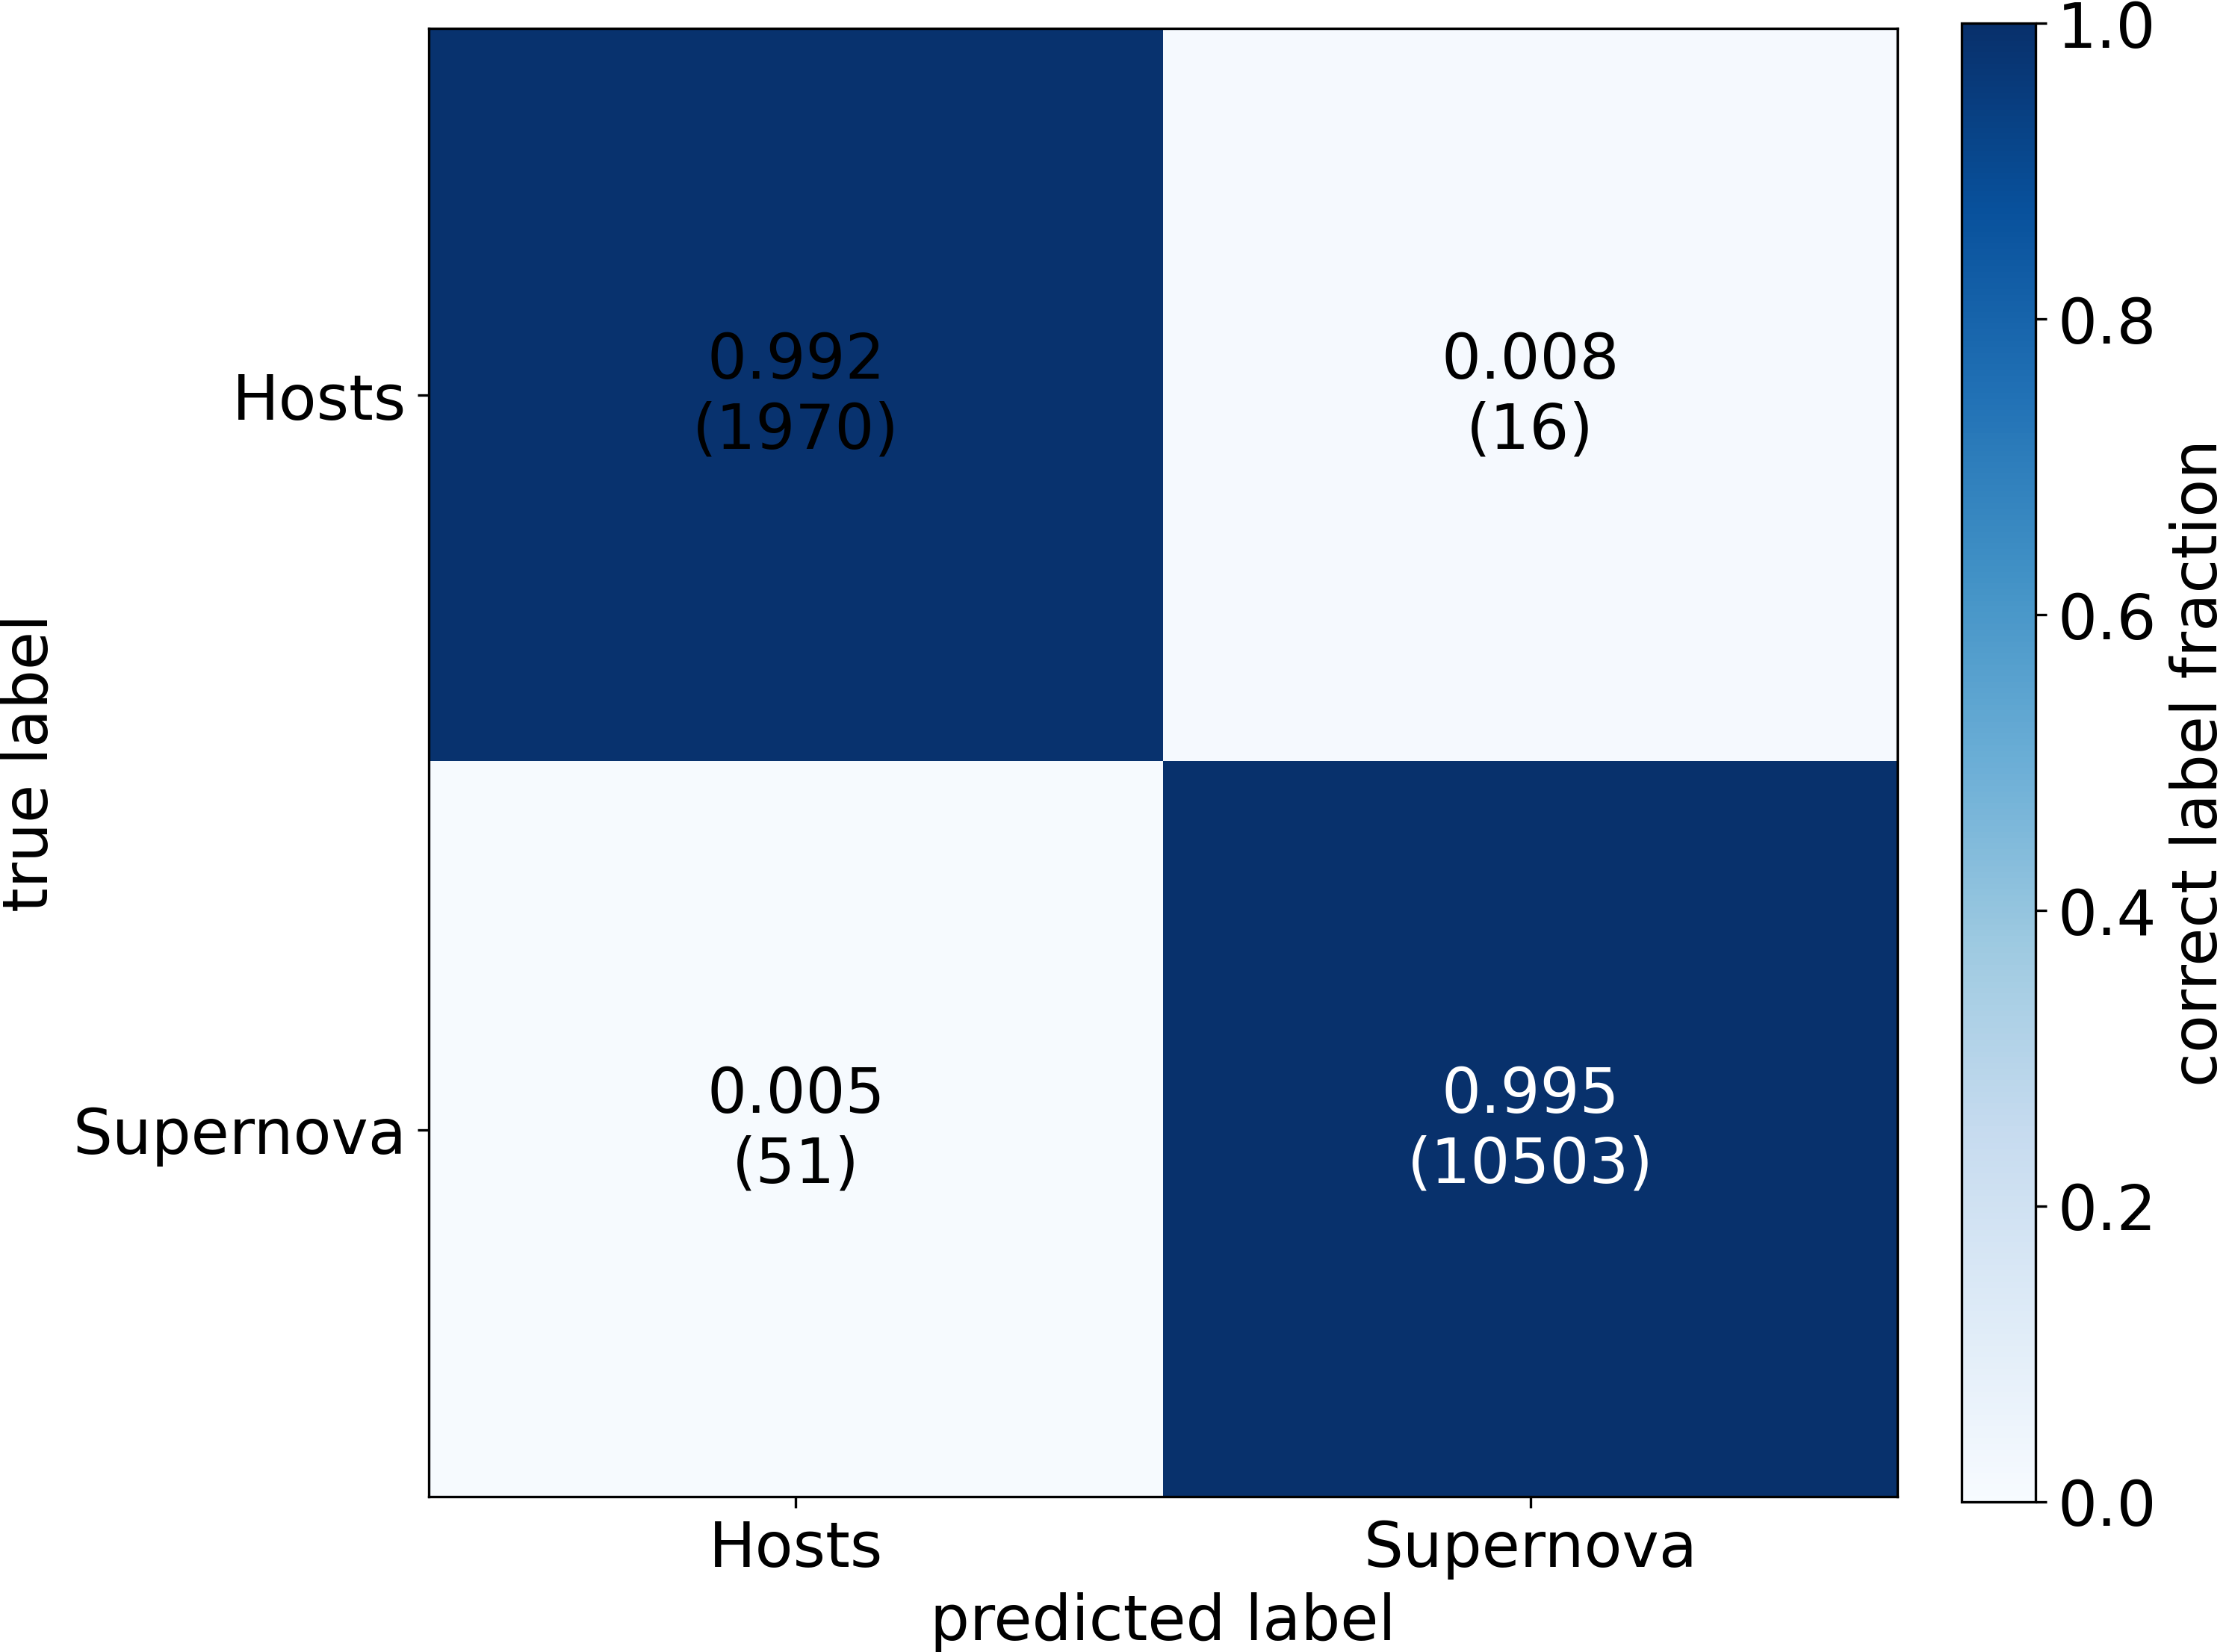
\includegraphics[height=4.2cm]{figures/v2_real/vit_model_V2cm9999_binary_e26.png}
%     \caption{Spectral ViT V2 Binary Diagnostics: ROC Curve (left) and Confusion Matrix (right) with a 99.99\% confidence
%     cut \label{fig:v2_binary_9999_qual}}
% \end{figure}




% References
\clearpage
% \addcontentsline{toc}{chapter}{Bibliography}
% \markboth{\MakeUppercase{Bibliography}}{}
\singlespacing
\printbibliography

\appendix
\chapter{Detailed Diagrams of Various Neural Networks}
\label{chap:NNArch}
%%%%%%%%%%%%%%%%%%%%%%%%%%%%%%%%%%%%%%%%%%%%%%%%%%%%%%%%%%%%%%%
\section{Multi-Layer Perceptron (Fully Connected Feed-Forward Networks)}
\label{app:MLP}


\section{Convolutional Neural Networks}
\label{app:CNN}


\section{Transformers}
\label{app:transformer}

\subsection{Spectral ViT}
\label{app:SpecViT}

\subsection{Multi-Head Attention}
\label{app:MHA}


\chapter{Title of Appendix B}


\end{document}
